%%%%%%%%%%%%%%%%%%%%%%%%%%%%%%%%%%%%%%%%%%%%%%%%%%%%%%%%%%%%%%%%%%%%%%
% Lớp 12 | Tọa độ của véc-tơ trong không gian | Tọa độ của véc-tơ và các công thức
% Dạng 2H2?2-6: Toán thực tế áp dụng các phép toán tọa độ hóa véc-tơ
% Số câu: 83  (sinh tự động bởi tach_cau.py; từ nay thầy sửa trực tiếp file này)
%%%%%%%%%%%%%%%%%%%%%%%%%%%%%%%%%%%%%%%%%%%%%%%%%%%%%%%%%%%%%%%%%%%%%%

%%%%%%%%%%%%%%%% TRẮC NGHIỆM 4 PHƯƠNG ÁN %%%%%%%%%%%%%%%%

% nguồn: Lop_12_Hinh_hoc_Chuong_2
\begin{ex}%[2H2N2-6]%[ma:c15a5339]
	Hình bên mô tả một sân cầu lông với kích thước theo tiêu chuẩn quốc tế. Với hệ toạ độ $Oxyz$ được thiết lập như hình bên (đơn vị trên mỗi trục là mét), giả sử $AB$ là một trụ cầu lông để căng lưới, hãy xác định tọa độ của  $B$.
	\begin{center}
		\begin{tikzpicture}[scale=0.8,font=\footnotesize,line join=round,line cap=round,>=stealth]
				 \coordinate (O) at (0,0);
				\coordinate  (Z) at (0,4);
				\coordinate (M) at (6,0); 
				\coordinate (N) at  (2,2);
				\coordinate (P) at ($(M)+(N)-(O)$); 
				\coordinate (A) at ($(P)!0.5!(N)$); 
				\coordinate (C) at  ($(O)!0.5!(M)$);
				 \coordinate (B) at ($(A)+(0,1)$);
				\coordinate (D) at ($(C)+(0,1)$); 
				\coordinate (E) at ($(A)!0.5!(B)$); 
				\coordinate (F) at  ($(C)!0.5!(D)$);
				\coordinate  (Y) at ($(O)!1.2!(N)$);
				 \coordinate (X) at ($(O)!1.2!(M)$);
				 \foreach \i/\g in {A/10,B/90,O/170}{\draw[fill=blue](\i) circle (1.5pt)
					 ($(\i)+(\g:5mm)$) node[scale=1]{$\i$};}
				\draw[->]  (O)--(Z);
				 \draw[->] (O)--(X);
				\draw[->]  (O)--(Y);
				\draw  (X) node[scale=1,below]{$x$};
				\draw  (Y) node[scale=1,above]{$y$};
				 \draw (Z) node[scale=1,left]{$z$};
				 \filldraw[green!90!black](O)--(N)--(P)--(M)--cycle;
				\draw (N)--(P)--(M) 
					(A)--(B)--(D)--(C) 
					(E)--(F); 
				\draw[pattern = north west  lines](F)--(D)--(B)--(E)--cycle;
				\draw[->]  ($(C)-(0,0.5)$)--($(O)-(0,0.5)$);
				\draw[->]  ($(C)-(0,0.5)$)--($(M)-(0,0.5)$);
				\draw ($(C)-(0,0.7)$)  node[scale=1,below]{$13{,}40m$};
				\draw[->] ($(M)!0.5!(P)$)+(0.5,0)--($(M)+(0.5,0)$); 
				\draw[->] ($(M)!0.5!(P)$)+(0.5,0)--($(P)+(0.5,0)$); 
				\draw ($(M)!0.5!(P)$)+(0.5,0) node[scale=1,right]{$6{,}10m$}; 
				\draw[->] ($(A)!0.5!(B)$)+(0.2,0)--($(B)+(0.2,0)$); 
				\draw[->]  ($(A)!0.5!(B)$)+(0.2,0)--($(A)+(0.2,0)$);
				\draw ($(A)!0.5!(B)$)+(0.2,0) node[scale=1,right]{$1{,}55m$}; 
			\end{tikzpicture}
	\end{center}
	\choice 
		{$\left(6{,}1; 6{,}7;  1{,}55\right)$}
		{\True $\left(6{,}7;  6{,}1; 1{,}55\right)$}
		{$\left(6{,}1;  0;1{,}55\right)$}
		 {$\left(0; 6{,}7; 1{,}55\right)$}
	 \loigiai{
		Toạ độ điểm $B\left(6{,}7; 6{,}1; 1{,}55\right)$. 
	 }
\end{ex}

% nguồn: Lop_12_Hinh_hoc_Chuong_2
\begin{ex}%[2H2H2-6]%[ma:be4bbcf7]
	Ở một sân bay, vị trí của máy bay được xác định bởi điểm $M$ trong không gian $Oxyz$ như hình bên. Gọi $H$ là hình chiếu vuông góc của  $M$ xuống mặt phẳng $\left(Oxy\right)$. Cho biết $OM=50$, $\left(\overrightarrow{i}, \overrightarrow{OH}\right)=64^{\circ}$, $\left(\overrightarrow{OH},\overrightarrow{OM}\right)=48^{\circ}$. Tìm toạ độ của điểm $M$.
	\begin{center}
		\begin{tikzpicture}[scale=0.8,font=\footnotesize,line join=round,line cap=round,>=stealth]
				\coordinate (O) at  (0,0);
				\coordinate (A) at  (-2,-2);
				\coordinate (B) at (6,0); 
				\coordinate (H) at ($(B)+(A)-(O)$); 
				\coordinate (C)  at ($(O)+(0,4)$);
				 \coordinate (M) at ($(C)+(H)-(O)$);
				\draw[dashed]  (A)--(H)--(M)--(C);
				\draw[dashed] (O)--(H)--(B); 
				\draw  (O)--(M);
				\foreach \i/\g in {O/110,A/90,B/90,C/180,M/0,H/-90}{\draw[fill=blue](\i) circle (1.5pt) 
					($(\i)+(\g:5mm)$)  node[scale=1]{$\i$};}
				 \coordinate (Z) at ($(O)+(0,5)$);
				\coordinate (Y) at ($(B)+(1,0)$); 
				\coordinate  (X) at ($(A)-(1,1)$);
				\draw[->] (O)--(Z); 
				\draw[->] (O)--(X); 
				\draw[->] (O)--(Y); 
				 \draw (X) node[scale=1,left]{$x$};
				\draw (Y)  node[scale=1,above]{$y$};
				\draw (Z) node[scale=1,left]{$z$}; 
				\pic[draw,thin,angle radius=2mm] {right angle = O--C--M}; 
				\pic[draw,thin,angle radius=2mm] {right angle  = O--A--H};
				\pic[draw,thin,angle radius=2mm] {right  angle = M--B--O};
				\pic[draw,thin,angle  radius=4mm] {angle = H--O--M};
				\pic[draw,thin,angle radius=6mm] {angle =  A--O--H};
				\draw ($(O)-(1,1)$)  node[scale=1,right]{$64^{\circ}$};
				 \draw ($(O)+(2,0)$) node[scale=1,below]{$48^{\circ}$};
				 \draw ($(O)!0.5!(M)$) node[scale=1,above]{$50$};
			\end{tikzpicture}
	\end{center}
	\choice 
		{$M\left(37{,}2; 14{,}7;  30{,}1\right)$}
		 {$M\left(14{,}7;37{,}2; 30{,}1\right)$}
		{$M\left(30{,}1; 14{,}7; 37{,}2\right)$} 
		{\True  $M\left(14{,}7; 30{,}1; 37{,}2\right)$}
	\loigiai{ 
		Tam giác $OMH$ vuông tại $H$ có  $OM=50$, góc $\widehat{MOH}=48^{\circ}$ nên ta có
		$OH=OM\cdot  \cos48^{\circ} \approx 33{,}5$; $OC=MH=OM\cdot \sin 48^{\circ} \approx 37{,}2$\\
		Tam giác $OAH$  vuông tại $A$, $OH=33{,}5$, $\widehat{AOH}=64^{\circ}$ nên ta có
		$OA=OH\cdot \cos64^{\circ} \approx 14{,}7$;  $OB=AH=OH\cdot \sin 64^{\circ} \approx 30{,}1$.\\
		Suy ra $\overrightarrow{OM}=\overrightarrow{OC}+\overrightarrow{OH}=\overrightarrow{OC}+\overrightarrow{OA}+\overrightarrow{OB}=14{,}7\cdot \overrightarrow{i}+30{,}1\cdot \overrightarrow{j}+37{,}2\cdot  \overrightarrow{k}$.\\
		Vậy $M\left(14{,}7; 30{,}1; 37{,}2\right)$. 
	} 
\end{ex}


%%%%%%%%%%%%%%%% ĐÚNG/SAI %%%%%%%%%%%%%%%%

% nguồn: Lop_12_Hinh_hoc_Chuong_2
\begin{ex}%[2H2H2-6]%[ma:979bff75]
	\immini[thm]{ 
	Hai chiếc khinh khí cầu bay lên từ  cùng một địa điểm. Chiếc thứ nhất cách điểm xuất phát $2$ km về phía nam và $1$ km về phía đông, đồng thời cách mặt đất $0{,}5$ km. Chiếc thứ hai nằm cách điểm xuất phát $1$ km về phía bắc và $1{,}5$ km về phía tây, đồng thời cách mặt đất $0{,}8$ km. Chọn hệ trục $Oxyz$ với gốc $O$ đặt tại điểm xuất phát của hai khinh khí cầu, mặt phẳng $Oxy$ trùng với mặt đất với trục $Ox$ hướng về phía nam, trục $Oy$ hướng về phía đông và trục $Oz$ hướng thẳng đứng lên trời (Hình minh họa), đơn vị đo lấy theo kilomet.}
	{\begin{tikzpicture}[scale=1,font=\footnotesize,line join=round,
			line  cap=round,>=stealth]
		\draw[->] (0:0) coordinate (A) node[below]{Bắc}--++(0:2) coordinate (O)  node[below]{$O$}--++(90:3) coordinate (C) node[left]{$z$}; \draw[->] (O)--++(0:3) coordinate (D) node[below]{$x$} node[above]{Nam};
		\draw[->](O)--++(40:2) coordinate  (X) node[above]{Tây}
			(O)--++(-140:2)  coordinate (X') node[below right]{Đông}node[left]{$y$};
		\draw[dashed](4,0) coordinate  (E)
			($(O)+(-140:1)$) coordinate (F)--($(E)+(F)-(O)$) coordinate  (G)--(E)
			(.6,0)  coordinate (M)
			($(O)+(40:1.3)$) coordinate (N)--($(M)+(N)-(O)$) coordinate  (K)--(M)
			(K)--++(90:1.3) coordinate  (P)--(O)
			 (G)--++(90:1) coordinate (Q)--(O);
		 \fill (O) circle (1pt);
		 \fill[red] (Q) circle (3pt);
		\fill[blue] (P)  circle (3pt);
	\end{tikzpicture}
	 }
	\choiceTF 
		{\True Với hệ tọa độ đã chọn, tọa  độ khinh khí cầu thứ nhất là $(2;1;0{,}5)$}
		{Với hệ tọa độ đã chọn, toạ độ  khinh khí cầu thứ hai là $(-1{,}5;-1; 0{,}8)$}
		{Khoảng cách từ điểm xuất phát đến khinh  khí cầu thứ nhất bằng $\sqrt{21}$ km}
		{\True Khoảng cách hai chiếc khinh khí cầu là $3{,}92$ km (\textit{kết quả làm tròn đến hàng phần trăm})} 
	\loigiai{ 
		\begin{itemchoice}
			\itemch Chiếc khinh khí cầu thứ nhất  có tọa độ là $(2;1;0{,}5)$.
			\itemch Chiếc khinh khí cầu thứ hai có tọa độ  là $(-1;-1{,}5; 0{,}8)$.
			\itemch Khoảng cách từ điểm xuất phát đến  khinh khí cầu thứ nhất bằng
			 $$\sqrt{2^2+1^2+0{,}5^2}=\dfrac{\sqrt{21}}{2}\mathrm{\,km}.$$
			\itemch Khoảng cách hai chiếc khinh khí cầu  là $$\sqrt{(-1-2)^2+(1{,}5-1)^2+(0{,}8-0{,}5)^2}=\sqrt{15{,}34} \approx 3{,}92\mathrm{\,km}.$$
		\end{itemchoice}
	 }
\end{ex}

% nguồn: Lop_12_Hinh_hoc_Chuong_2
\begin{ex}%[2H2C2-6]%[ma:606f0af8]
	\immini[thm]{Hình  minh họa sơ đồ một ngôi nhà trong hệ trục tọa độ $Oxyz$, trong đó nền nhà, bốn bức tường và hai mái nhà đều là hình chữ nhật.
	\choiceTF 
		{Tọa độ  của các điểm $A\left(5;0;0\right)$}
		{\True Tọa độ  của các điểm $H\left(0;5;3\right)$}
		 {\True Chiều cao của ngôi nhà là $4$}
		{\True Góc nhị diện có cạnh là đường thẳng $FG$, hai mặt lần lượt là $\left(FGQP\right)$ và $\left(FGHE\right)$ gọi là góc dốc của mái nhà. Số  đo của góc dốc của mái nhà bằng $26{,}6^\circ$ (làm tròn kết quả đến hàng phần mười của độ)}}
		{\begin{tikzpicture}[scale=.6,font=\tiny,line join=round,line cap=round,>=stealth]
		\def\a{5} 
		\path 
			(0:0) coordinate  (O)
			 (0:\a) coordinate (A)
			 ++(40:\a/2) coordinate (B)
			++(180:\a)  coordinate (C)
		\foreach \x in {O,A,B,C}{(\x)++(90:\a/1.2) coordinate (\x')} 
			 ($(O')+(20:\a/1.6)$) coordinate (P)
			($(C')+(20:\a/1.6)$) coordinate (Q) 
			 ($(O)!1.5!(C)$) coordinate (y)
			 ($(O)!1.5!(A)$) coordinate (x)
			($(O)!1.5!(O')$)  coordinate (z);
		 \draw (O)--(A)--(A')--(O')--cycle
			(A)--(B)--(B')--(A') 
			(O')--(C')--(Q)--(P)--cycle 
			 (P)--(A')--(B')--(Q);
		\draw[dashed] (O)--(C)--(B) 
			(C)--(C')--(B'); 
		\draw[->,dashed] (C)--(y) node[above] {$y$}; 
		\draw[->] (A)--(x)  node[below] {$x$};
		\draw[->]  (O')--(z) node[right] {$z$};
		 \draw (O) node[below]{$O (0; 0; 0)$}
			(O')  node[left]{$E (0; 0; 3)$}
			(B) node[right]{$B (4; 5; 0)$} 
			(B') node[right]{$G  (4; 5; 3)$}
			(P) node[right]{$P (2; 0;  4)$}
			(Q) node[above]{$Q (2; 5;  4)$}
			(A)  node[below]{$A$}
			(C) node[left]{$C$} 
			 (C') node[left]{$H$}
			(A') node[right]{$F$}; 
	\end{tikzpicture}
		 }
	 \loigiai{
		\begin{itemchoice}
			\itemch Vì nền nhà là hình chữ nhật nên tứ giác $OABC$ là hình chữ nhật, suy ra $x_A=x_B=4,y_C=y_B=$ 5. Do $A$ nằm  trên trục $Ox$ nên tọa độ điểm $A$ là $\left(4;0;0\right)$.
			 \itemch Tường nhà là hình chữ nhật, suy ra $y_H=y_C=5,z_H=z_E=3$.\\
			Do $H$ nằm trên mặt phẳng $\left(Oyz\right)$ nên tọa độ điểm $H$  là $\left(0;5;3\right)$.
			\itemch Chiều  cao của ngôi nhà bằng cao độ của điểm $P$ suy ra $h=4$.
			\itemch Để tính góc đốc của mái nhà, ta tính số đo của góc nhị diện có cạnh là đường  thẳng $FG$, hai mặt lần lượt là $(FGQP)$ và $(FGHE)$.\\
			Do mặt phẳng $(Ozx)$ vuông góc với hai mặt phẳng $(FGQP)$ và $(FGHE)$ nên $\widehat{PFE}$  là góc phẳng nhị diện cần tìm.\\
			Ta có $\overrightarrow{FP}=(-2;0;1)$, $\overrightarrow{FE}=(-4;0;0)$.\\ 
			$\cos \widehat{PFE} =\cos \left( \overrightarrow{FP},\overrightarrow{FE} \right) =\dfrac{\overrightarrow{FP} \cdot \overrightarrow{FE}}{\left|\overrightarrow{FP}\right| \cdot \left|\overrightarrow{FE}\right|} =\dfrac{(-2)(-4)+0  \cdot 0+1 \cdot 0}{\sqrt{(-2)^2+0^2+1^2} \cdot \sqrt{(-4)^2+0^2+0^2}} =\dfrac{2\sqrt{5}}{5}$.\\
			Do đó, $\widehat{PFE}  \approx 26{,}6^\circ $. \\
			Vậy  góc đốc mái nhà khoảng $ 26{,}6^\circ $.
		\end{itemchoice}
	} 
\end{ex}


%%%%%%%%%%%%%%%% TRẢ LỜI NGẮN %%%%%%%%%%%%%%%%

% nguồn: Lop_12_Hinh_hoc_Chuong_2
\begin{bt}%[2H2H2-6]%[ma:6e07fcd6]
	Hình vẽ bên minh họa hình ảnh một tòa nhà trong không gian với hệ tọa độ $Oxyz$ (đơn vị trên mỗi trục tọa độ là mét). Biết $OABC.DEFG$ là hình chóp cụt có hai đáy  nằm trên hai mặt phẳng song song, $OABC$ là hình chữ nhật nằm trong mặt phẳng $(Oxy)$, $OA=100$\,m, $OC=60$\,m, và điểm $D(10;10;8)$. Khoảng cách từ $B$ đến mặt phẳng $(OCGD)$ bằng bao nhiêu mét? (kết quả làm tròn đến hàng phần chục)?
	\begin{center}
		 \tdplotsetmaincoords{120}{135}
		\begin{tikzpicture}[tdplot_main_coords,>=stealth,font=\footnotesize,scale=1]
				 \path
					(5,0,0) coordinate  (A)
					(5,3,0)  coordinate (B)
					(0,3,0)  coordinate (C)
					(.5,0,2) coordinate (D) 
					(3.5,0,2) coordinate (E) 
					 (3.5,1.5,2) coordinate (F)
					(.5,1.5,2)  coordinate (G)
					(0,0,0) coordinate  (O);
				\draw[fill=blue!20,opacity=.3]  (O)--(A)--(E)--(F)--(G)--(C)--cycle;
				\draw[dashed] (A)--(B)--(C) 
					 (B)--(F);
				\draw (O)--(D)--(E) 
					(D)--(G); 
				\draw[->] (O)--(6,0,0)  node[below right]{$x$};
				 \draw[->] (O)--(0,4,0) node[left]{$y$};
				\draw[->] (O)--(0,0,4)  node[right]{$z$};
				\foreach  \i/\j in {O/-90,A/-45,B/35,C/-135,D/80,E/20,F/90,G/150}
				\fill (\i) circle (1pt) 
					node[tdplot_screen_coords,shift={(\j:.25)}]{$\i$}; 
			\end{tikzpicture}
	\end{center}
	\shortans{62,5} 
	\loigiai{Từ  hình vẽ ta có $B(100;60;0)$, $C(0;60;0)$ và $O(0;0;0)$.\\
		 Ta có $\vec{OC}=(0;60;0)$, $\vec{OD}=(10;10;8)$.\\
		Véc-tơ pháp tuyến của mặt phẳng $(OCGD)$ là 
		$$\vec{n} = \left[\vec{OC},\vec{OD}\right]= (60\cdot 8 - 0\cdot 10; 0\cdot 10 -  0\cdot 8; 0\cdot 10 - 60\cdot 10) = (480;0;-600).$$
		 Chọn $\vec{n}' = \dfrac{1}{120}\vec{n} = (4;0;-5)$.\\
		Mặt phẳng $(OCGD)$ đi qua điểm $O(0;0;0)$ nên phương trình là  $4x-5z=0$.\\
		Khoảng cách từ $B(100;60;0)$ đến mặt phẳng  $(OCGD)$ là:
	$$\mathrm{d}(B,(OCGD))=\dfrac{|4\cdot 100 -  5\cdot 0|}{\sqrt{4^{2}+(-5)^{2}}} = \dfrac{400}{\sqrt{41}} \approx 62{,}5\mathrm{m}.$$}
\end{bt}

% nguồn: Lop_12_Hinh_hoc_Chuong_2
\begin{bt}%[2H2H2-6]%[ma:5a6cee3f]
	Một tháp trung tâm kiểm soát không lưu ở sân bay cao 80 m sử dụng ra đa có phạm vi theo dõi $500$ km được đặt trên đỉnh tháp. Chọn hệ trục toạ độ $Oxyz$ có gốc $O$ trùng với vị trí chân tháp, mặt phẳng $(Oxy)$ trùng với mặt đất sao cho trục $Ox$ hướng về phía tây, trục $Oy$ hướng về phía nam, trục $Oz$ hướng thẳng đứng lên phía trên (Hình)  (đơn vị trên mỗi trục tính theo kilômét).
	\begin{center}
	\definecolor{deepskyblue}{rgb}{0.0, 0.75, 1.0} 
	 \definecolor{arsenic}{rgb}{0.23, 0.27, 0.29}
	\definecolor{antiquewhite}{rgb}{0.98, 0.92,  0.84}
	\definecolor{green(ryb)}{rgb}{0.4,  0.69, 0.2}
		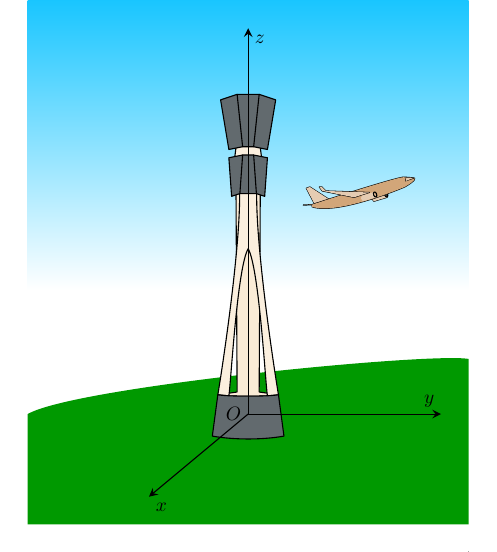
\begin{tikzpicture}[>=stealth,line join=round,line cap=round,scale=.7,transform shape]
				\tikzset{san_co/.pic={ 
				\def\D{ 
					(-4,-2) 
					..controls +(30:1)  and +(170:.7)..(4,-1)--(4,-4)--(-4,-4)
					--cycle; 
				} 
				\fill[green!60!black] \D; 
					}} 
				\fill[bottom color=white,top color=deepskyblue!90,middle color=white] (-4,-5) rectangle  (4,5.5);
				 \tikzset{co_vat/.pic={
				 \def\Tr{
					(-.55,-1.65)..controls +(-10:.2)  and +(-170:.2)..(.55,-1.65)--(.2,-1.6)--(.22,2)--(-.22,2)--(-.2,-1.6)--cycle;
				} 
				\fill[antiquewhite]  \Tr;
				 \draw\Tr;
				 \def\T{
					 (-.2,3)--(-.25,2.6)
					..controls  +(-50:.5) and +(80:.2)..(-.55,-1.65)--(-.35,-1.67)
					..controls +(80:.2) and  +(-120:.4)..(0,1)
					..controls +(-60:.4)  and +(100:.2)..(.35,-1.67)--(.55,-1.65)
					..controls +(100:.2) and +(-130:.5)..(.25,2.6)--(.2,3)--cycle; 
				 }
				 \fill[antiquewhite!80] \T;
				 \draw\T;
				 \def\A{
					(-.5,3.7)--(-.35,2.8)--(-.1,2.85)--(.1,2.85)--(.35,2.8)--(.5,3.7)--(.2,3.8)--(-.2,3.8)--cycle 
					 (.1,2.7)--(-.1,2.7)--(-.35,2.65)--(-.3,1.95)--(-.15,2)--(.15,2)--(.3,1.95)--(.35,2.65)--(.1,2.7)
					(-.55,-1.65) 
					..controls +(-10:.2) and  +(-170:.2)..(.55,-1.65)--(.65,-2.4)
					..controls +(-170:.4) and  +(-10:.4)..(-.65,-2.4)--cycle;
				} 
				 \fill[arsenic!80] \A;
				\draw\A; 
				 \draw (.2,3.8)--(.1,2.85)
					 (-.2,3.8)--(-.1,2.85)
					 (.1,2.7)--(.15,2)
					 (-.1,2.7)--(-.15,2);
				\def\xmin{0}  \def\xmax{3.5}
				\def\ymin{-2}  \def\ymax{5}
				 \draw[->] (\xmin,-2)--(\xmax,-2) node [above left]{\normalsize $y$};
				\draw[->]  (0,\ymin)--(0,\ymax) node [below right]{\normalsize $z$};
				\draw[->] (0,-2)--++(-1.8,-1.5) node  [below right]{\normalsize $x$};
				\node  at (0,-2) [left]{$O$};
					 }}
				\tikzset{may_bay/.pic={ 
				\def\D{(-2,-.45)--(-2.36,.24)--(-2.2,.3)--(-1.35,-.25)--cycle;} 
				\draw \D; 
				\fill[brown!40!]  \D;
				 \def\Q{
					 (.15,-.1)
					..controls +(-140:0.1) and +(140:0.1).. (.2,-.35) 
					--(.8,-.17)--(.7,.07)--cycle; 
				} 
				\draw  \Q;
				\draw[xshift=.5cm] \Q; 
				\fill[brown!40!,xshift=.5cm]  \Q;
				 \draw[rotate=-70,xshift=-.23cm,yshift=1.27cm] (.7,-.1) ellipse (.12cm and 0.07cm);
				\def\T{(-2.1,-.5) 
					..controls +(40:0) and +(-170:0.7).. (2,.74) 
					..controls +(-40:0) and +(170:0.3)..  (2.55,.7)
					..controls +(-150:0)  and +(30:.65).. (2.1,.3)
					 ..controls +(-150:0) and +(-18:1.25).. (-2.1,-.6)
					..controls +(90:0)  and +(-90:0).. (-2.1,-.51)
					 --(-2.5,-.52)--cycle;
				 }
				 \draw \T;
				\fill[brown!70!] \T; 
				 \def\C{(.5,.05)
					..controls +(170:0) and +(-10:0)..  (-1.48,.12)
					..controls  +(-80:0) and +(170:0.02).. (-1.65,.3)
					..controls +(180:0) and +(0:0).. (-1.77,.3) 
					..controls  +(-80:0) and +(110:0).. (-1.64,.12)
					..controls +(-35:0) and  +(145:0).. (-.2,-.17)
					 --cycle;
				 }
				\draw  \C;
				\fill[brown!40!]  \C;
				\fill[brown!40!] \Q; 
				 \draw[rotate=-70,xshift=-.4cm,yshift=.8cm] (.7,-.1) ellipse (.12cm and 0.07cm);
				\draw  (2.18,0.73)--(2.5,0.7)--(2.14,0.58)--cycle;
				\fill[brown!40!](2.18,0.73)--(2.51,0.71)--(2.14,0.57)--cycle; 
					}} 
				 \pgfresetboundingbox
				\path (0,0) pic[scale=1]{san_co} 
					 (0,0) pic[scale=1]{co_vat}
					(2,2) pic[scale=.4]{may_bay}; 
			\end{tikzpicture}
	\end{center}
	Một máy bay tại vị trí $A$ cách mặt đất $10$ km, cách  $300$ km về phía đông và $200$ km về phía bắc so với tháp trung tâm kiểm soát không lưu. Tính khoảng cách từ máy bay đến ra đa (làm tròn kết quả đến hàng đơn vị).
	\shortans{361} 
	 \loigiai{
		Theo giả thiết, ra đa  ở vị trí có toạ độ $I(0;0;0{,}08)$; điểm $A(-300;-200;10)$.\\
		Vậy khoảng cách  từ máy bay đến ra đa là
		\begin{center}
			$IA=\sqrt{(-300-0)^2+(-200-0)^2+(10-0{,}08)^2}\approx  361$ (km).
		\end{center}
	} 
\end{bt}

% nguồn: Lop_12_Hinh_hoc_Chuong_2
\begin{bt}%[2H2H2-6]%[ma:d4c0c8bc]
	Một người điều khiển Flycam đang đứng tại một điểm được xem là gốc tọa độ $O(0; 0; 0)$ trong không gian. Các trục tọa độ được quy ước như sau: Trục $Ox$ theo hướng Đông; trục $Oy$ theo hướng Bắc; trục $Oz$ theo hướng thẳng đứng lên trên; đơn vị mỗi trục là mét. Tại một thời điểm, Flycam ở vị trí $A$ có tọa độ $(1;-8;4)$. Khoảng cách (đường chim bay) từ người  điều khiển đến Flycam tại vị trí $A$ là mấy mét?
	\shortans{9} 
	 \loigiai{
		Người điều khiển ở  $O(0,0,0)$. Flycam ở $A(1,-8,4)$.\\
		 Khoảng cách\allowdisplaybreaks
		\begin{eqnarray*}
			OA &=& \sqrt{(1-0)^2  + (-8-0)^2 + (4-0)^2}\\
			&=& \sqrt{1^2 + (-8)^2 +  4^2}\\
			&=& \sqrt{1 + 64 +  16}\\
			&=&  \sqrt{81} \\
			&=& 9\quad  (\text{m}).
		\end{eqnarray*}
	} 
\end{bt}

% nguồn: Lop_12_Hinh_hoc_Chuong_2
\begin{bt}%[2H2H2-6]%[ma:f57ddd85]
	Trong không gian $Oxyz$ (đơn vị trên mỗi trục tọa độ là mét), một ngôi nhà như hình vẽ dưới đây có sàn nhà nằm ngang trên mặt  phẳng $(\alpha) \colon 2x+y-3z+18=0$. Hai mái nhà lần lượt nằm trên các mặt phẳng $(P) \colon x-y=0$, $(Q) \colon x+y-2z=0$. Hỏi chiều cao của ngôi nhà tính từ sàn nhà đến nóc nhà (điểm cao nhất của mái nhà) là bao nhiêu? (làm tròn đến hàng phần chục).
	\begin{center}
	\definecolor{airforceblue}{rgb}{0.36, 0.54, 0.66} 
	\definecolor{burntsienna}{rgb}{0.91, 0.45, 0.32} 
	 \definecolor{anti-flashwhite}{rgb}{0.95, 0.95, 0.96}
	\definecolor{brown(web)}{rgb}{0.65, 0.16, 0.16} 
		\begin{tikzpicture}[line join=round,line cap=round,scale=1,transform shape]
				\tikzset{mai_nha/.pic={ 
				\clip (-.9,-3.5)--(3,-3.4)--(2.5,0)--cycle; 
				\draw[fill=burntsienna] 
					 (0,0)
					foreach \n in {1,2,...,15}{-- ++ (-.5,0) -- ++ (.5,.5) -- ++ (1,0) --  ++ (-.5,-.5)} -- cycle
					(-0.25,-.5) 
					foreach \n in  {1,2,...,15}{-- ++ (-.5,0) -- ++ (.5,.5) -- ++ (1,0) -- ++ (-.5,-.5)} -- cycle
					 (-.5,-1)
					foreach \n in {1,2,...,15}{-- ++ (-.5,0) -- ++ (.5,.5) -- ++ (1,0) -- ++  (-.5,-.5)} -- cycle
					(-.75,-1.5) 
					foreach \n  in {1,2,...,15}{-- ++ (-.5,0) -- ++ (.5,.5) -- ++ (1,0) -- ++ (-.5,-.5)} -- cycle
					 (-1,-2)
					foreach \n in {1,2,...,15}{-- ++ (-.5,0) -- ++ (.5,.5)  -- ++ (1,0) -- ++ (-.5,-.5)} -- cycle
					(-1.25,-2.5) 
					foreach \n in {1,2,...,15}{--  ++ (-.5,0) -- ++ (.5,.5) -- ++ (1,0) -- ++ (-.5,-.5)} -- cycle
					(-1.5,-3) 
					foreach \n in {1,2,...,15}{-- ++ (-.5,0) -- ++ (.5,.5) -- ++ (1,0) --  ++ (-.5,-.5)} -- cycle
					(-1.75,-3.5) 
					foreach \n in  {1,2,...,15}{-- ++ (-.5,0) -- ++ (.5,.5) -- ++ (1,0) -- ++ (-.5,-.5)} -- cycle;
					}} 
				\tikzset{mai_nha_2/.pic={ 
				 \clip (.8,-3.5)--(5.7,-3.5)--(6.2,.05)--(4,-.7)--cycle;
				 \draw[fill=burntsienna]
					(0,0) 
					foreach \n in {1,2,...,15}{-- ++ (-.5,0) -- ++ (.5,.5) -- ++ (1,0) -- ++ (-.5,-.5)}  -- cycle
					 (-0.25,-.5)
					foreach \n in  {1,2,...,15}{-- ++ (-.5,0) -- ++ (.5,.5) -- ++ (1,0) -- ++ (-.5,-.5)} -- cycle
					 (-.5,-1)
					foreach \n in {1,2,...,15}{-- ++ (-.5,0) -- ++ (.5,.5) -- ++ (1,0) -- ++ (-.5,-.5)} -- cycle 
					(-.75,-1.5) 
					foreach \n in {1,2,...,15}{-- ++ (-.5,0) -- ++ (.5,.5) -- ++ (1,0) -- ++  (-.5,-.5)} -- cycle
					(-1,-2) 
					foreach \n in {1,2,...,15}{-- ++ (-.5,0)  -- ++ (.5,.5) -- ++ (1,0) -- ++ (-.5,-.5)} -- cycle
					 (-1.25,-2.5)
					foreach \n in {1,2,...,15}{-- ++ (-.5,0) -- ++  (.5,.5) -- ++ (1,0) -- ++ (-.5,-.5)} -- cycle
					(-1.5,-3) 
					foreach \n in {1,2,...,15}{-- ++ (-.5,0) -- ++ (.5,.5) -- ++ (1,0) -- ++ (-.5,-.5)} --  cycle
					 (-1.75,-3.5)
					foreach \n in {1,2,...,15}{-- ++ (-.5,0) -- ++ (.5,.5) --  ++ (1,0) -- ++ (-.5,-.5)} -- cycle;
					}} 
				 \tikzset{tuong_lon/.pic={
				 \draw[fill=brown] (-4.5,-.9)--(-4.5,1.7)--(2,.32)--(2,-1);
				\draw[pattern= horizontal lines]  (-4.5,-.9)--(-4.5,1.7)--(2,.32)--(2,-1);
					 }}
				\tikzset{tuong_nho/.pic={ 
				\draw[fill=brown] (-4.6,-4)--(2,-4.5)--(2,.5)--(-4.6,-.13)--cycle; 
					}} 
				 \tikzset{cua_so/.pic={
				\draw  (-.5,.4) rectangle (0,1.4);
				\draw[color=anti-flashwhite,line width=.6mm] (-.5,.4) rectangle (0,1.4); 
				 \draw[color=anti-flashwhite,line width=.3mm] (-.35,.4)--(-.35,1.4)
					(-.15,.4)--(-.15,1.4) 
					 (-.5,.6)--(0,.6)
					 (-.5,.9)--(0,.9)
					 (-.5,1.2)--(0,1.2);
				\fill[anti-flashwhite] (0,.4) rectangle (.3,1.4); 
				 \fill[anti-flashwhite] (-.8,.4) rectangle (-.5,1.4);
					 }}
				\path  (-3.4,4.4) pic[yscale=1,xscale=1.2,yslant=-.22]{mai_nha}
					(7,4.78)  pic[yscale=1,xscale=-1.2,yslant=-.16]{mai_nha_2}
					(4,0)  pic[xscale=.9,yslant=.37,yscale=1.2]{tuong_lon}
					 (-1.3,.4) pic[scale=1.8,scale=.35,yslant=-.25]{tuong_nho}
					(2,-2)  pic[scale=1.5,yslant=.2]{cua_so}
					 (4.8,-1.15) pic[scale=1.2,yslant=.2]{cua_so};
				 \draw[fill=airforceblue,yslant=-.32] (-3,-2.73) --(-3,-.5)-- (-1,-.3)--(-1,-2.75);
			\end{tikzpicture}
	\end{center}
	 \shortans{4,8}
	\loigiai{Chiều cao của ngôi nhà là khoảng cách từ đường thẳng giao tuyến của hai mặt phẳng mái nhà $(P)$ và $(Q)$ đến mặt phẳng sàn  nhà $(\alpha)$.\\
		Cần tìm tọa độ một điểm thuộc đường thẳng giao tuyến của hai mặt phẳng $(P)$ và $(Q)$,  ta có $\heva{&x-y=0 \\&x+y-2z=0.}$\\
		Cho  $y=0$, ta giải hệ phương trình
		 $$\heva{&x=0\\&x-2z=0} \Leftrightarrow \heva{&x=0\\&z=0.}$$
		Do  đó gốc tọa độ $O(0;0;0)$ thuộc đường thẳng giao tuyến của hai mặt phẳng $(P)$ và $(Q)$.\\
		Khi đó chiều cao  từ sàn nhà đến nóc nhà là $\mathrm{d}(O;(\alpha))$
		$$\mathrm{d}(O;(\alpha))=\dfrac{|2\cdot 0+1\cdot 0-3\cdot 0+18|}{\sqrt{2^{2}+1^{2}+(-3)^{2}}} = \dfrac{18}{\sqrt{14}} = \dfrac{9\sqrt{14}}{7}\approx  4{,}8\mathrm{m}.$$
	 }
\end{bt}

% nguồn: Lop_12_Hinh_hoc_Chuong_2
\begin{bt}%[2H2H2-6]%[ma:53e43728]
	Trong không gian, xét hệ toạ độ $Oxyz$ có gốc $O$ trùng với vị trí của một giàn  khoan trên biển, mặt phẳng $(Oxy)$ trùng với mặt biển (được coi là phẳng) với trục $Ox$ hướng về phía tây, trục $Oy$ hướng về phía nam và trục $Oz$ hướng thẳng đứng lên trời. Đơn vị đo trong không gian $Oxyz$ lấy theo kilômét. Một chiếc ra đa đặt tại giàn khoan có phạm vi theo dõi là $30$ (km). Khi một chiếc tàu thám hiểm có toạ độ là $(25;15;0)$ đối với hệ toạ độ nói trên thì khoảng cách giữa tàu và ra đa là bao nhiêu kilômét? (làm tròn kết quả đến chữ số thập phân thứ nhất).
	\shortans{29,2} 
	\loigiai{ 
		Theo đề ta có tọa độ  của ra đa là $(0;0;0)$ tọa độ của tàu thám hiểm là $(25;15;0)$.\\
		Khi đó khoảng cách giữa ra  đa và tàu thám hiểm là
		\[d=\sqrt{(25-0)^2+(15-0)^2+(0-0)^2}=5\sqrt{34}\approx 29{,}2\text{ (km).}\] 
	 }
\end{bt}

% nguồn: Lop_12_Hinh_hoc_Chuong_2
\begin{bt}%[2H2H2-6]%[ma:986193fe]
	Trong một trò chơi mô phỏng bắn súng, một người chơi đặt điểm ngắm tại điểm là giao điểm của $AC$ và $BD$ trong căn phòng hình hộp chữ nhật $ABCD.A'B'C'D'$ có kích thước $AB=15$\,m, $AD=20$\,m, $AA'=25$\,m. Người chơi di chuyển trên đoạn $BD$ có nhiệm vụ bắn trúng một mục  tiêu di động trên mặt phẳng $(CB'D')$. Tính khoảng cách ngắn nhất từ điểm ngắm đó đến mục tiêu (làm tròn đến chữ số thập phân thứ nhất).
	\begin{center}
		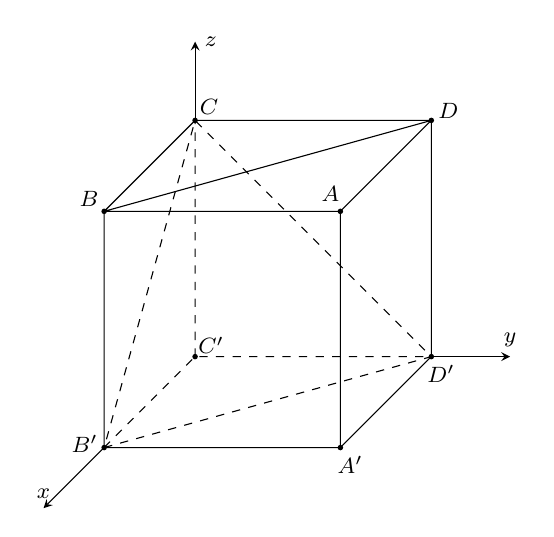
\begin{tikzpicture}[>=stealth,rotate around x=-90,rotate around z=-90,font={\footnotesize},scale=1]
				\path (0,0,0) coordinate (C') 
					(3,0,0) coordinate (B') 
					(3,3,0) coordinate (A') 
					(0,3,0) coordinate  (D')
					(0,0,3) coordinate  (C)
					(3,0,3) coordinate  (B)
					(3,3,3) coordinate  (A)
					 (0,3,3) coordinate (D);
				\draw  (A)--(B)--(C)--(D)--(A)--(A')--(B')--(B)
					 (A')--(D')--(D)--(B);
				\draw[dashed]  (B')--(C')--(D')
					(C')--(C) 
					(B')--(D')--(C)--cycle; 
				\draw[->] (B')--++(2,0,0) node[above]{$x$}; 
				\draw[->]  (D')--++(0,1,0) node[above]{$y$};
				\draw[->] (C)--++(0,0,1)  node[right]{$z$};
				\foreach \i/\j in  {A/120,B/140,C/45,D/30,A'/-60,B'/170,C'/35,D'/-60}
				\fill (\i) circle (1pt)  node[shift={(\j:2.5mm)}]{$\i$};
			\end{tikzpicture}
	\end{center}
	\shortans{10,8} 
	\loigiai{Chọn hệ trục tọa độ $C'xyz$ như hình vẽ  ($C'$ là gốc tọa độ), ta có\\ $C'(0;0;0)$,
		$B'(20;0;0),\quad D'(0;15;0),\quad C(0;0;25),\quad B(20;0;25),\quad  D(0;15;25).$\\
		Phương trình mặt phẳng $(B'CD')$ là phương trình đoạn  chắn
		$$\dfrac{x}{20}+\dfrac{y}{15}+\dfrac{z}{25}=1 \Leftrightarrow  15x+20y+12z-300=0.$$
		Do $BD \parallel  (B'CD')$, suy ra $\mathrm{d}(BD,(B'CD'))=\mathrm{d}(B,(B'CD')) =\mathrm{d}(C',(B'CD')).$\\
		Khoảng cách ngắn nhất từ điểm bắn  đến mục tiêu chính là khoảng cách từ $BD$ đến mặt phẳng $(B'CD')$. Do vậy ta có
		$$\mathrm{d}(C',(B'CD')) =  \dfrac{|-1|}{\sqrt{\dfrac{1}{20^{2}}+\dfrac{1}{15^{2}}+\dfrac{1}{25^{2}}}} \approx 10{,}8\mathrm{m}.$$
	Vậy khoảng cách ngắn nhất từ điểm ngắm đến  mục tiêu là khoảng $10{,}8$\,m.}
\end{bt}

% nguồn: Lop_12_Hinh_hoc_Chuong_2
\begin{bt}%[2H2H2-6]%[ma:ccf08ce6]
	Cho hình chữ nhật $ABCD$  có $AB=2BC$, gọi $N$ là điểm nằm trên cạnh $CD$ sao cho $AC\perp BN$. Tính tỉ số $\dfrac{DN}{CN}$.
	\shortans{3} 
	 \loigiai{
		\begin{center}
			\begin{tikzpicture}
					\def  \c{2} \def \g{-90};
					\draw (0,0) coordinate (A) 
						--(\g:\c) coordinate (B)--++(0:2*\c) coordinate (C)--++(180+\g:\c) coordinate (D)--(A)--(C); 
					\path  ($(A)!0.3!(D)$) coordinate (N)
						(intersection of B--N and  A--C) coordinate (H);
					\draw (B)--(N); 
					\foreach \x/\g in {A/90,B/-90,C/-90,D/90,H/10,N/90} 
					 \fill (\x) circle (1pt)
						($(\x)+(\g:3mm)$) node{\x}; 
					 \draw pic [draw,angle radius = 2mm]{right angle = A--H--B};
				\end{tikzpicture}
		\end{center}
		Đặt $\overrightarrow{CN}=x\cdot \overrightarrow{CD}$, $(x>0)$ và $BC=a; CD=2a$, $(a>0)$.\\ 
		Ta có $\overrightarrow{CA}=\overrightarrow{CB}+\overrightarrow{CD}$; $\overrightarrow{BN}=\overrightarrow{CN}-\overrightarrow{CB} 
		=x\cdot  \overrightarrow{CD}-\overrightarrow{CB}$.\\
		 Theo giả thiết ta có
		\begin{eqnarray*}
			 \overrightarrow{CA}\cdot \overrightarrow{BN}=0
			&\Leftrightarrow& \left(\overrightarrow{CB}+\overrightarrow{CD}\right)\left(x\cdot  \overrightarrow{CD}-\overrightarrow{CB}\right)=0 \\
			&\Leftrightarrow&  x\cdot CD^2-CB^2=0
			 \Leftrightarrow x=\dfrac{CB^2}{CD^2}=\dfrac{a^2}{4a^2}=\dfrac{1}{4}\cdot
		\end{eqnarray*}
		Suy ra  $DN=3CN$ hay $\dfrac{DN}{CN}=3$.
	} 
\end{bt}

% nguồn: Lop_12_Hinh_hoc_Chuong_2
\begin{bt}%[2H2H2-6]%[ma:b343ce25]
	Trong hệ trục toạ độ $Oxyz$ cho trước (đơn vị trên trục là mét), cho một trạm thu phát sóng 5G có bán kính vùng phủ sóng của trạm ở ngưỡng $600$\,m được đặt ở vị trí $I(200;450;60)$. Tìm giá trị lớn nhất của $m$ (làm tròn đến hàng đơn vị) để một người dùng điện thoại ở vị trí $M(m+100;m+370;0)$ có thể sử dụng dịch vụ của trạm nói  trên.
	\shortans{512} 
	 \loigiai{
		Để người dùng  điện thoại ở vị trí $M(m+100;m+370;0)$ có thể sử dụng dịch vụ của trạm nói trên thì
		\allowdisplaybreaks 
		\begin{eqnarray*}
			 IM \le 600&\Leftrightarrow&\sqrt{(m-100)^2+(m-80)^2+(-60)^2} \le 600\\
			&\Leftrightarrow&(m-100)^2+(m-80)^2+(-60)^2 \le 360\,000\\ 
			&\Leftrightarrow&2m^2-360m+20\,000 \le  360\,000\\
			&\Leftrightarrow&2m^2-360m-340\,000 \le  0\\
			&\Leftrightarrow&m^2-180m-170\,000 \le  0\\
			&\Leftrightarrow&90-\sqrt{178\,100} \le m \le  90+\sqrt{178\,100}.
		\end{eqnarray*}
		Vậy giá trị lớn nhất của $m$ (làm tròn đến hàng đơn vị) để một người dùng điện thoại ở vị trí $M(m+100;m+370;0)$ có thể sử dụng dịch vụ của trạm nói trên là  \[m=90+\sqrt{178\,100}\approx 512\,\text{ (m).}\]
	} 
\end{bt}

% nguồn: Lop_12_Hinh_hoc_Chuong_2
\begin{bt}%[2H2H2-6]%[ma:acfb97e8]
	Trên phần mềm mô phỏng việc điều khiển drone giao hàng trong không gian $Oxyz$. Một đội gồm ba drone giao hàng $A$, $B$ và $C$ đang có toạ độ là $A(1;1;1)$, $B(5;7;9)$, $C(9;11;4)$. Gọi $d_1$, $d_2$, $d_3$ lần lượt là khoảng cách giữa mỗi cặp drone  giao hàng trên. Tính $d_1+d_2+d_3$. (kết quả làm tròn đến hàng phần chục)
	\definecolor{battleshipgrey}{rgb}{0.52,  0.52, 0.51}
	\definecolor{gainsboro}{rgb}{0.86, 0.86, 0.86} 
	\definecolor{moonstoneblue}{rgb}{0.45, 0.66, 0.76} 
	\definecolor{arsenic}{rgb}{0.23, 0.27, 0.29} 
	\definecolor{pastelorange}{rgb}{1.0,  0.7, 0.28}
	\definecolor{anti-flashwhite}{rgb}{0.95,  0.95, 0.96}
	\definecolor{capri}{rgb}{0.0,  0.75, 1.0}
	\begin{center}
		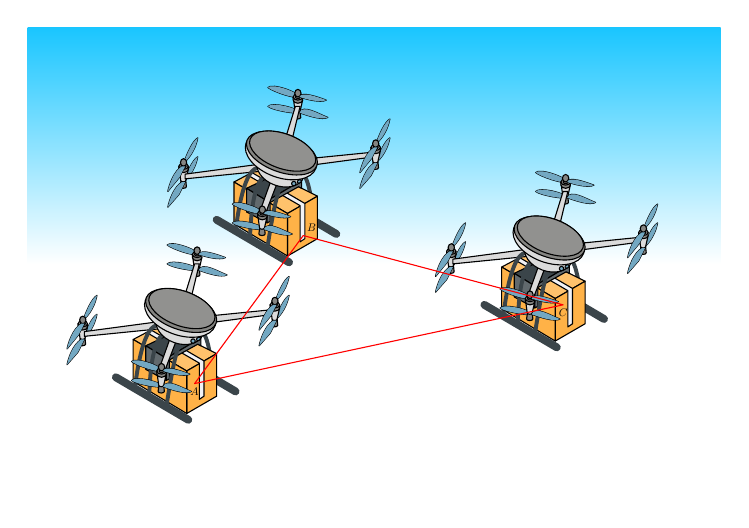
\begin{tikzpicture}[line join=round,line cap=round,scale=0.4,transform shape]
				\clip (-8,-10)  rectangle (14,5);
				\fill[top  color=capri!90,bottom color=white,middle color=white] (-8,-10) rectangle (14,5);
				\tikzset{than/.pic={ 
				\draw[arsenic,line  width=.5mm] (.75,.3)
					..controls  +(-10:.2) and +(100:.1)..(1.1,-1.1);
				\draw[arsenic,line width=1mm] (-1,0.1)--(1.8,-1.55); 
				\draw[fill=pastelorange!80] (-1.45,.1)--(.25,-.9)--(1.2,-.35)--(-.6,.55)--cycle; 
				 \draw[fill=pastelorange] (.25,-.9)--(.25,-2.25)--(1.2,-1.7)--(1.2,-.35)--cycle;
				\draw[fill=anti-flashwhite] (-1.02,.32)--(.65,-.65)--(.65,-1.8)--(.8,-1.7)--(.8,-.58)--(-.88,.4)--cycle; 
				 \draw[fill=pastelorange] (-1.45,.1)--(.25,-.9)--(.25,-2.25)--(-1.45,-1.23)--cycle;
				\draw[fill=arsenic]  (-1.05,-.1)--(0,.4)--(.7,.15)--(-.4,-.5)--cycle;
				\draw[fill=arsenic!80] (-1.05,-.1)--(-.4,-.5)--(-.4,-1.2)--(-1.05,-.85)--cycle; 
				 \draw[fill=arsenic!80] (-.4,-1.2)--(-.4,-.5)--(.7,.15)--(.7,-.1)--(.6,-.05)--(-.3,-.55)--(-.3,-1.15)--cycle;
				\draw[fill=gainsboro]  (-3,.35)--(0,.75)--(3,1.05)--(3,.9)--(0,.5)--(-3,.2)--cycle;
				 \draw[fill=gainsboro] (-.65,-.9)--(-.45,-.9)--(.3,1.05)--(.65,2.5)--(.5,2.5)--(.05,1.05)--cycle;
				\draw[arsenic,line width=.5mm] (-.7,.55) 
					..controls +(-170:.5) and +(80:.2)..(-1.4,-1.45); 
				\draw[arsenic,line width=.5mm] (-.35,.35) 
					..controls  +(-170:.6) and +(80:.2)..(-.95,-1.73);
				\draw[arsenic,line width=.5mm]  (.1,.05)
					..controls +(-170:.2) and +(80:.2)..(-.4,-2.05); 
				\draw[arsenic,line  width=1mm] (-2,-1.1)--(.3,-2.45);
				\draw[fill=gainsboro,rotate=160] (.15,-.5) ellipse  (.78cm and 0.55cm);
				\draw[fill=moonstoneblue](.45,.05) circle  (2pt);
				 \draw[rotate=30,yscale=.7,fill=moonstoneblue](.6,-.3) circle (2pt);
				 \draw[fill=gainsboro,rotate=160] (.28,-.9) ellipse (1.18cm and 0.7cm);
				\draw[fill=battleshipgrey,rotate=160] (.28,-.98) ellipse  (1.18cm and 0.6cm);
				\draw[fill=battleshipgrey!90,rotate=160] (.28,-1.05) ellipse  (1.1cm and 0.55cm);
					}} 
				\tikzset{quat1/.pic={ 
				\def\T2{ 
					 (-3.05,.7)
					..controls  +(70:.3) and +(-150:.2)..(-2.6,1.5)
					..controls  +(-100:.3) and +(40:.3)..cycle
					(-3.05,.1) 
					..controls  +(70:.3) and +(-150:.2)..(-2.6,.9)
					..controls +(-100:.3) and +(40:.3)..cycle; 
				} 
				\draw\T2; 
				\fill[moonstoneblue]  \T2;
				\draw[fill=battleshipgrey]  (-2.98,.15)--(-2.96,-.05) arc (0:-180:.1cm and 0.05cm)--(-3.13,.15)--cycle;
				\draw[fill=gainsboro] (-2.9,.5)--(-2.98,.15) arc (0:-180:.08cm and  0.05cm)--(-3.2,.6)--cycle;
				\draw[fill=battleshipgrey] (-2.9,.6)--(-2.9,.5) arc (0:-180:.15cm  and 0.1cm)--(-3.2,.6)--cycle;
				\draw[fill=battleshipgrey!80]  (-3.05,.6) ellipse (.15cm and 0.1cm);
				 \draw[fill=battleshipgrey] (-3.05,.6) ellipse (.08cm and 0.05cm);
				\draw[fill=battleshipgrey,rotate=90] (.72,3.05) ellipse (.12cm  and 0.1cm);
				 \def\T1{
					 (-3.1,.6)
					 ..controls +(-150:.3) and +(80:.2)..(-3.55,-.2)--(-3.18,.25)--(-3,.6)--cycle
					(-3.1,.1) 
					..controls  +(-150:.3) and +(80:.2)..(-3.55,-.7)--(-3.2,-.3)--(-3,.1)--cycle;
				 }
				 \draw\T1;
				 \fill[moonstoneblue] \T1;
					 }}
				\tikzset{quat2/.pic={ 
				 \def\T3{
					 (-3,.1)
					..controls  +(-150:.1) and +(-40:.2)..(-4,.3)
					..controls  +(50:.2) and +(100:.15)..cycle
					(-3,.6) 
					..controls +(-150:.15)  and +(-40:.2)..(-4,.9)
					..controls +(50:.2) and +(100:.15)..cycle; 
				 }
				 \draw\T3;
				\fill[moonstoneblue]  \T3;
				 \draw[fill=battleshipgrey] (-2.98,.15)--(-2.96,-.05) arc (0:-180:.1cm and 0.05cm)--(-3.13,.15)--cycle;
				\draw[fill=gainsboro] (-2.9,.5)--(-2.98,.15) arc  (0:-180:.08cm and 0.05cm)--(-3.2,.6)--cycle;
				\draw[fill=battleshipgrey]  (-2.9,.6)--(-2.9,.5) arc (0:-180:.15cm and 0.1cm)--(-3.2,.6)--cycle;
				\draw[fill=battleshipgrey!80] (-3.05,.6)  ellipse (.15cm and 0.1cm);
				\draw[fill=battleshipgrey] (-3.05,.6) ellipse (.08cm and  0.05cm);
				 \draw[fill=battleshipgrey,rotate=90] (.72,3.05) ellipse (.12cm and 0.1cm);
				\def\T4{ 
					 (-3,.6)
					..controls +(-20:.2) and +(-150:.2)..(-2.15,.5) 
					..controls  +(160:.3) and +(70:.2)..cycle
					(-3,.1) 
					 ..controls +(-20:.3) and +(-150:.2)..(-2.1,-.05)
					 ..controls +(160:.3) and +(70:.3)..cycle;
				 }
				 \draw\T4;
				\fill[moonstoneblue] \T4; 
					}} 
				\def\dx{8.5} 
				 \def\dy{-2.7}
				\def\mx{-3.2} 
				\def\my{-5} 
				\path 
					 (0,0) pic[scale=1]{quat1}
					(3.63,2.2) pic[scale=1]{quat2} 
					(0,0) pic[scale=1]{than} 
					(2.5,-1.5)  pic[scale=1]{quat2}
					(6.1,.6) pic[scale=1]{quat1} 
					(\dx,\dy) pic[scale=1]{quat1} 
					 (3.63+\dx,2.2+\dy) pic[scale=1]{quat2}
					(\dx,\dy) pic[scale=1]{than} 
					 (2.5+\dx,-1.5+\dy) pic[scale=1]{quat2}
					 (6.1+\dx,.6+\dy) pic[scale=1]{quat1}
					 (\mx,\my) pic[scale=1]{quat1}
					(3.63+\mx,2.2+\my) pic[scale=1]{quat2} 
					 (\mx,\my) pic[scale=1]{than}
					 (2.5+\mx,-1.5+\my) pic[scale=1]{quat2}
					 (6.1+\mx,.6+\my) pic[scale=1]{quat1};
				\path (.75,-1.6) coordinate (B) 
					(9,-3.8) coordinate  (C)
					(-2.7,-6.3) coordinate (A); 
				\node at  (B) [above right]{$B$};
				\node at  (A) [below]{$A$};
				\node  at (C) [below]{$C$};
				\draw[red] (B)--(C)--(A)--cycle; 
			\end{tikzpicture}
	\end{center}
	 \shortans{31,5}
	 \loigiai{
		Ta có 
		\begin{itemize}
			\item $\overrightarrow{AB}=(4;6;8)$,  suy ra $AB=\sqrt{4^2+6^2+8^2}=2\sqrt{29}$.
			\item $\overrightarrow{AC}=(8;10;3)$, suy ra  $AC=\sqrt{8^2+10^2+3^2}=\sqrt{173}$.
			 \item $\overrightarrow{BC}=(4;4;-5)$, suy ra $BC=\sqrt{4^2+4^2+(-5)^2}=\sqrt{57}$.
		\end{itemize}
		Khi đó $d_1+d_2+d_3=2\sqrt{29}+\sqrt{173}+\sqrt{57}\approx 31{,}5$. 
	} 
\end{bt}

% nguồn: Lop_12_Hinh_hoc_Chuong_2
\begin{bt}%[2H2H2-6]%[ma:b9888563]
	Trong không gian với một hệ trục tọa độ cho trước (đơn vị đo: ki-lô-mét), ra-đa phát hiện một chiếc máy bay di chuyển với vận tốc và hướng không đổi từ điểm $A(800;500;7)$ đến điểm $B(940;550;8)$ trong $10$ phút. Nếu máy bay tiếp tục giữ nguyên vận tốc và hướng  bay thì tọa độ của máy bay sau $10$ phút tiếp theo là $D(x;y;z)$. Khi đó $x+y+z$ bằng bao nhiêu?
	 \shortans{1689}
	 \loigiai{
		\begin{center}
			\begin{tikzpicture}[scale=1,font=\footnotesize,line join=round,line cap=round,>=stealth]
					 \path
						(0:0) coordinate  (D)
						+(0:5)  coordinate (C)
						 +(65:3) coordinate (O)
						($(O) + (0,4)$) coordinate (E) 
						 ($(O)+(C)-(D)$) coordinate (B)
						($(E)+(C)-(O)$)  coordinate (F) node{\Large \faPlane}
						 ($(O)!1.2!(D)$) coordinate (M)
						($(O)!1.2!(B)$) coordinate  (N)
						($(O)!1.2!(E)$) coordinate (K); 
					\foreach \x/\y/\t in {O/M/x,O/N/y,O/K/z} 
					 \draw[->]
						(\x)--(\y)  node[right]{$\t$};
					 \draw[dashed]
						(E) --  (F) --(C)
						(O)--(C) 
						 (D)--(C)--(B);
					 \foreach \x/\g/\t in {D/180/800,O/180/O,B/90/500,E/180/7}
					\fill  (\x) circle (1.5pt)
						+(\g:3mm) node{$\t$}; 
					\foreach  \x/\y/\z in {O/E/F,O/D/C,O/B/C}{
						\draw[thin] pic[draw,angle radius = 6pt]{right angle  = \x--\y--\z};
					} 
					\node at  (F) [rotate=280,scale=1.5] {\Large \faPlane};
				\end{tikzpicture}
		\end{center}
		\begin{itemize}
			\item Vị trí của  máy bay sau $10$ phút tiếp theo là $D(x;y;z)$.
			\item Vì hướng  của máy bay không đổi nên $\overrightarrow{AB}$ và $\overrightarrow{BD}$ cùng hướng.
			\item Do vận tốc của máy bay không đổi và thời gian bay từ $A$ đến $B$ bằng thời gian bay từ $B$ đến $D$  nên $AB = BD$.
			\item Do đó $\overrightarrow{BD} = \overrightarrow{AB} = \left( 940-800; 550-500;  8-7 \right) = (140; 50; 1)$.
			\item Mặt khác, $\overrightarrow{BD} = (x - 940; y - 550; z - 9)$ nên $\heva{x& - 940 &=& 140 \\ y& - 550 &=& 50  \\ z& - 8 &=& 1}$.
			\item Giải hệ phương trình trên ta được $\heva{x&=1080\\y&=600\\z&=9}$  nên $x+y+z=1080+600+9=1689$.
		\end{itemize}
	} 
\end{bt}

% nguồn: Lop_12_Hinh_hoc_Chuong_2
\begin{bt}%[2H2H2-6]%[ma:593f287f]
	Mô phỏng trong không gian với hệ tọa độ $Oxyz$ (đơn vị trên mỗi trục số là kilômét), một máy bay đang ở vị trí $A(6;-8;1)$ và sẽ hạ cánh ở điểm có tọa độ $O(0;0;0)$ trên đường băng. Có một lớp mây mỏng được mô phỏng bởi một mặt phẳng đi qua ba điểm $P(12;0;0)$,  $Q(0;-12;0)$ và $R(0;0;1,2)$. Tính khoảng cách giữa máy bay và đường băng ngay khi máy bay bay xuyên qua lớp mây (kết quả làm tròn đến hàng phần trăm của kilômét).
	\begin{center}
		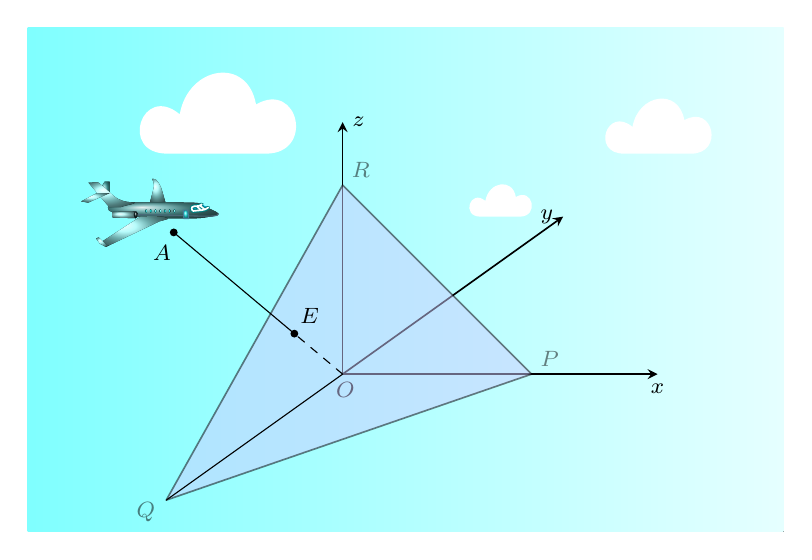
\begin{tikzpicture}[scale=0.4,font=\footnotesize,line join=round,line cap=round,>=stealth]
				 \tikzset{Icon-Maybay/.pic={
				\begin{scope}
					\fill[ball color  =cyan!40!gray,rounded corners=0.02](-5.6,3)--++(60:0.8)--++(2:0.55)--++(-90:2)--cycle;
					 \fill[ball color =cyan!90!gray!40!white](-0.4,1.5)..controls++(75:2) and++(-68:0.75)..(-0.15,4)--++(-5:0.35)..controls++(-50:0.95) and++(106:2)..(1.25,1.5)--cycle;
					\fill[ball color =cyan!30!gray](-4.85,1)..controls++(-90:0.6) and++(180:0.2)..(-4,0.5)--++(-12:3.3)--++(0:4)..controls++(0:2) and++(-172:1)..(6,0)..controls++(8:1)  and++(-90:0.1)..(6.85,0.3)..controls++(90:0.2) and++(-30:1)..(5,1.3)..controls++(90:0.25) and++(0:8)..(-4,1.5)--cycle;
					\draw[cyan!40!black](6.85,0.3) coordinate  (mui)..controls++(-90:0.5) and++(0:6)..(-2,0.2);
					\fill[ball color  =cyan!90!gray!40!white,rounded corners=0.02](-1.8,0)--++(-5:0.35)--++(-147:4.85)--++(-50:0.7)--++(25.5:6.5)..controls++(-155.5:0.5) and++(-170:0.15)..(1.5,-0.25)..controls++(120:0.5) and++(2:1)..(-1.8,0);
					\fill[ball color =cyan!90!gray!40!white,rounded corners=0.02](-6.1,-2.3)--++(-54:0.7)--++(-28:0.7)--++(25.5:.35)--++(-180:.2)--++(135:1.2)--cycle; 
					\fill[ball color =cyan!90!gray!40!white,rounded corners=0.02](-6.9,3.6)--++(2:1)..controls++(-35:2) and++(178:2.3)..(-2,1.5)..controls++(-90:0.2)  and++(20:1)..(-3.5,1)--++(180:1.2)--cycle;
					\fill[ball color =cyan!90!gray!40!white,rounded corners=0.02](-6,2.5)--++(0:1.35)--++(-156:2.5)--++(170:0.75)--cycle; 
					\fill[ball  color =cyan!70!gray!40!white,rounded corners=0.02](-1.9,-0.17)--++(90:0.72)--++(181:2.45)--++(-90:0.6)--cycle;
					\fill[ball color =cyan!90!gray!10!black,line width=0.02,draw,cyan!30!black,rounded corners=0.005](-1.9,-0.18) arc (-90:270:0.2  and 0.38);
					\fill[cyan](5.05,1.3)--++(-25:0.8)..controls++(-140:0.55) and++(10:0.5)..(4.2,0.6)..controls++(180:0.15)  and++(182:0.45)..(4.3,1.1)..controls++(2:0.5) and++(-135:0.2)..(5.1,1.3);
					\draw[draw,teal,double,distance=0.03](5.05,1.3)++(-26:0.8)..controls++(-140:0.55) and++(10:0.5)..(4.2,0.6) foreach \i in{1,2,...,4}{coordinate[pos=\i/4](B\i)}..controls++(180:0.15) and++(182:0.45)..(4.3,1.1)..controls++(2:0.5) and++(-135:0.2)..(5.1,1.3) foreach \i  in{1,2,...,10}{coordinate[pos=\i/10](A\i)}
						 (A2)--(B2)
						 (A6)--(B1);
					\foreach \i in {0,1,...,6} 
					\fill[ball color=cyan](-0.8+0.5*\i,0.4) arc (-90:270:0.1 and 0.2); 
				\fill[draw,cyan!10!teal,ball color=cyan!80!gray,rounded corners=0.015](3.2,-0.2)--++(95:0.9)--++(0:0.5)--++(-85:0.9)--cycle; \end{scope}
					}} 
				 \tikzset{Icon-may/.pic={
				 \def\r{0.25}
				\fill[white,line width=2.5*\r pt](-\r,0)--(\r,0)..controls++(0:\r) and  ++(30:\r)..(0.8*\r,\r)..controls++(100:\r) and ++(80:\r)..(-0.75*\r,0.8*\r)..controls++(140:\r) and++(180:\r)..(-\r,0);
					}} 
				\fill[left  color=cyan!50,right color=cyan!10](-12,-7) rectangle (12,9);
				\path (3,3)  pic{Icon-may}
					(8,5) pic[scale=1.7]{Icon-may} 
					(-6,5)  pic[scale=2.5]{Icon-may}
					 (-8,3) pic[scale=0.12]{Icon-Maybay};
				\begin{scope}[semithick]
					 \draw[-stealth](-2,-2) node[shift={(-80:.2)}]{$O$}--(8,-2) node[below]{$x$};
					\draw[-stealth](-2,-2)--(5,3) coordinate[pos=-.8] (Q)  node[left]{$y$};
					\draw[-stealth](-2,-2)--(-2,6) node[right]{$z$}; 
					\draw[fill=blue!20,opacity=.5] (4,-2) coordinate (P) node[shift={(40:.3)}]{$P$} 
						--(Q) node[shift={(-150:.3)}]{$Q$}--(-2,4)  node[shift={(40:.3)}]{$R$}--cycle;
				\end{scope}
				\draw[dashed] (-2,-2)--++(140:2) coordinate (E) node[circle,fill,inner  sep=1pt]{} node[shift={(50:.3)}]{$E$};
				\draw  (-2,-2)--(Q)
					(E)--++(140:5)  node[circle,fill,inner sep=1pt]{} node[shift={(-120:.3)}]{$A$};
			\end{tikzpicture}
	\end{center}
	\shortans{5,02} 
	\loigiai{Mặt phẳng $(PQR)$ đi qua ba điểm $P(12;0;0)$, $Q(0;-12;0)$, $R(0;0;1,2)$ nên phương trình đoạn chắn của mặt  phẳng $(PQR)$ là
		$$\dfrac{x}{12}+\dfrac{y}{-12}+\dfrac{z}{1,2}=1 \Leftrightarrow x-y+10z-12=0.$$ 
		Gọi $E(x_{0};y_{0};z_{0})$ là giao  điểm của quỹ đạo $OA$ và mặt phẳng $(PQR)$.\\
		Vì $\vec{OE}$ và $\vec{OA}$ cùng phương nên tồn tại số thực $t\in[0;1]$  sao cho $\vec{OE}=t\vec{OA} \Leftrightarrow \heva{&x_{0}=6t\\ &y_{0}=-8t\\&z_{0}=t.}$ \\
		Do điểm $E\in (PQR)$  nên ta có $$x_{0}-y_{0}+10z_{0}-12=0\Leftrightarrow 6t-(-8t)+10t-12=0 \Leftrightarrow t=\dfrac{1}{2}.$$
		Suy ra $\heva{&x_{0}=3\\ &y_{0}=-4\\ &z_{0}=0{,}5}  \Rightarrow E(3;-4;0,5)$.\\
		Khoảng cách giữa máy bay và đường băng (gốc $O$) ngay khi xuyên qua  lớp mây là
	$$OE=\sqrt{3^{2}+(-4)^{2}+(0{,}5)^{2}}=\sqrt{25{,}25}\approx  5{,}02.$$}
\end{bt}

% nguồn: Lop_12_Hinh_hoc_Chuong_2
\begin{bt}%[2H2H2-6]%[ma:da96dc1d]
	Trong giờ thể dục học về kỹ thuật chuyền bóng hơi, Bình và An tập chuyền bóng cho nhau. Ở một  động tác Bình chuyền bóng cho An, quả bóng bay lên cao nhưng lại lệch sang bên trái của An và rơi xuống vị trí cách chỗ An đứng $0{,}5$\,m và cách chỗ Bình $4{,}5$\,m. Chọn hệ trục tọa độ $Oxyz$ sao cho gốc tọa độ $O$ tại vị trí của Bình, vị trí của An nằm trên tia $Ox$ và mặt phẳng $Oxy$ là mặt đất (tham khảo hình vẽ). Biết rằng quỹ đạo của quả bóng nằm trong mặt phẳng $(\alpha) \colon x+by+cz+d=0$ và $(\alpha)$ vuông góc với mặt đất. Khi đó, giá trị của $-5b^{2}-c^{2}+3d^{2}$ bằng bao nhiêu?
	\begin{center}
		\begin{tikzpicture}[line join = round,line cap=round,>=stealth,font=\footnotesize,scale=1]
				\draw[->] (2,2) coordinate (O) -- (7.5,2)  coordinate (x);
				\draw[->] (2,2) -- (0.6,0.8) coordinate (y); 
				\draw[->] (2,2)  -- (2,5.2) coordinate (z);
				\fill (2.3,3.1) circle (2pt); 
				\draw[dashed] (2.3,3.1)..  controls +(28:3.0) and +(90:1).. (6.55,1.35) coordinate (H);
				\fill (H) circle (2pt)  node[above right] {$A$};
				\fill  (1.9,2.85) circle (3pt);
				\draw[line width=3pt] (1.9,2.85) -- (2.0,2.6) -- (2.0,2.3) -- (1.8,2.1) 
					(2.0,2.3) --  (2.05,2.2) -- (2.0,2.0)
					(2.0,2.75) --  (2.2,2.95);
				\fill (6.65,2.7) circle (3pt); 
				\draw[line width=3pt] 
					(6.65,2.7) -- (6.85,2.4) -- (6.75,2.2) --  (6.95,2.0)
					(6.85,2.4) -- (6.65,2.3) -- (6.65,2.0) 
					 (6.7,2.6) -- (6.5,2.5)
					(6.7,2.6) -- (6.5,2.4); 
				 \draw (O)--(H)--($(O)!(H)!(x)+(0.13,0)$) coordinate (t);
				\draw pic[draw,angle radius=2mm] {right angle =  O--t--H};
				\path 
					($(t)+(-0.7,-0.25)$)  node {$0{,}5~\mathrm{m}$}
					($(O)+(2,-0.75)$) node  {$4{,}5~\mathrm{m}$};
				\foreach \p/\r in {O/-90,x/90,y/90,z/180} 
				 \fill (\p) node[shift={(\r:3mm)}] {$\p$};
			\end{tikzpicture}
	\end{center}
	 \shortans{-400}
	\loigiai{Quả bóng rơi xuống tại điểm $A(\sqrt{20};0,5;0)$.\\ 
		Mặt phẳng $(\alpha) \colon  x+by+cz+d=0$ đi qua $O(0;0;0)$ nên $d=0$.\\
		Điểm $A(\sqrt{20};0,5;0)$  thuộc $(\alpha)$ nên có
		$$\sqrt{20}+0,5b=0 \Leftrightarrow b=-2\sqrt{20}  \Leftrightarrow b=-4\sqrt{5}$$
		Mặt khác $(\alpha)$ vuông góc với mặt đất (mặt phẳng $Oxy$  có $\vec{n}_{(Oxy)}=\vec{k}=(0;0;1)$) nên
		\[\vec{n}_{(\alpha)}\perp\vec{n}_{(Oxy)} \Leftrightarrow \vec{n}_{(\alpha)}\cdot\vec{k}=0 \Leftrightarrow  c=0.\]
		Vậy mặt phẳng $(\alpha)$ có phương  trình là $(\alpha) \colon x-4\sqrt{5}y=0$.\\
		Giá trị cần tính  là
	 $$-5b^{2}-c^{2}+3d^{2} = -5\cdot (-4\sqrt{5})^{2} - 0^{2} + 3\cdot (0)^{2} = -5\cdot (80) = -400.$$}
\end{bt}

% nguồn: Lop_12_Hinh_hoc_Chuong_2
\begin{bt}%[2H2H2-6]%[ma:f6777c41]
	Hai chiếc máy bay không người lái cùng bay lên tại một địa điểm. Sau một thời gian bay, chiếc máy bay thứ nhất cách  điểm xuất phát về phía Bắc $20$ km và về phía Tây $10$ km, đồng thời cách mặt đất $0{,}7$ km. Chiếc máy bay thứ hai cách điểm xuất phát về phía Nam $30$ km và về phía Đông $25$ km, đồng thời cách mặt đất $1$ km. Xác định khoảng cách giữa hai chiếc máy bay. (\textit{Kết quả làm tròn đến hàng đơn vị})
	\shortans{61} 
	\loigiai{Chọn hệ trục tọa độ $Oxyz$, với gốc đặt tại điểm xuất phát của hai chiếc máy bay, mặt phẳng $(Oxy)$ trùng với mặt đất, trục $Ox$ hướng về phía Bắc, trục $Oy$ hướng về phía Tây, trục $Oz$ hướng thẳng đứng lên trời, đơn vị  đo lấy theo kilômét (xem hình vẽ).
		\begin{center}
			\begin{tikzpicture}[scale=0.7,font=\footnotesize,line join=round,line cap=round,>=stealth]
					 \pgfmathsetmacro\a{3/sqrt (2)}
					 \path
						(0,0)  coordinate [label=left:$O$](O)
						(O)+(-135:3) coordinate [label=left:$B$](B) 
						($(O)+(4,0)$) coordinate  (N)
						($(B)+(N)-(O)$) coordinate (E) 
						($(O)+(0,4)$) coordinate (G) 
						($(E)+(0,4)$) coordinate  (A);
					\draw[->] (O)--($(O)+(6,0)$) node[above] {$y$} node[below]  {Tây};
					\draw[->] (O)--($(O)+(-135:4)$) node[left] {$x$} node[right] {Bắc}; 
					\draw[->] (0,0)--(0,5)  node[left]{$z$};
					\draw[dashed]  (B)--(E)--(N)
						(E)--(A)--(G); 
					\foreach \diem in {A,E,B,N,G,O}  \fill (\diem) circle (1.5pt);
				\end{tikzpicture}
		\end{center}
		Chiếc máy bay thứ nhất có tọa độ $(20;10;0{,}7)$.\\ 
		Chiếc máy bay thứ hai có tọa độ $(-30;-25;1)$.\\ 
		Do đó khoảng cách giữa hai chiếc  máy bay là $$\sqrt{(20+30)^2+(10+25)^2+(0,7-1)^2} \approx 61~(\mathrm{km}).$$
	} 
\end{bt}

% nguồn: Lop_12_Hinh_hoc_Chuong_2
\begin{bt}%[2H2V2-6]%[ma:c8018e17]
	Một chiếc máy bay không người lái bay lên tại một điểm. Sau một thời gian bay, chiếc máy bay cách điểm xuất phát về phía Bắc $55$ km và về phía Tây $20$ km, đồng thời cách mặt đất $1{,}5$ km. Khi đó khoảng cách của chiếc máy bay với vị trí xuất phát bằng bao nhiêu kilômét? (kết quả làm tròn  đến hàng phần chục).
	\shortans{58,5} 
	\loigiai{ 
	\immini{Chọn hệ trục tọa độ $Oxyz$, với gốc toạ độ $O$ đặt tại điểm xuất phát chiếc máy bay, mặt phẳng $(Oxy)$ trùng với mặt đất, trục $Ox$ hướng về  phía Bắc, trục $Oy$ hướng về phía Tây, trục $Oz$ hướng thẳng đứng lên trời, đơn vị đo lấy theo kilômét (như hình vẽ).\\
		Khi đó chiếc máy bay có tọa độ là $A\left(20; 55;  1{,}5\right)$.\\
		Và $\overrightarrow{OA}=\left(20; 55; 1{,}5\right)$, suy ra $OA=\sqrt{20^2+55^2+\left(1{,}5^2\right)}\approx  58{,}5$.\\
		Vậy  chiếc máy bay cách vị trí xuất phát $58{,}5$ kilômét.}
		{\begin{tikzpicture}[scale=1,font=\footnotesize,line join=round,line cap=round,>=stealth]
		\def\len{3.5} 
		\path  (0,0,0) node[left] {$O$};
		\draw[->] (0,0,0) -- (\len,0,0)  node[below] {Tây} node[above] {$y$};
		\draw[->] (0,0,0)  -- (0,\len,0) node[right] {Trời} node[above left] {$z$};
		\draw[->] (0,0,0) -- (0,0,\len) node[above left] {Bắc} node[below  right] {$x$};
		\coordinate (B) at (0,0,\len-1); 
		\coordinate (T)  at (\len-1,0,0);
		\coordinate (TR)  at (0,\len-1,0);
		\coordinate (TB) at ($(B)+(T)$); 
		\coordinate (TRTB) at  ($(TR)+(TB)$);
		 \draw[dashed] (B)--(TB)--(T)
			(0,0,0)--(TB)--(TRTB)--(TR); 
		\foreach  \diem in {B,T,TB,TR,TRTB} \fill (\diem) circle (1pt);
	\end{tikzpicture}
		 }
	 }
\end{bt}

% nguồn: Lop_12_Hinh_hoc_Chuong_2
\begin{bt}%[2H2V2-6]%[ma:d73f9940]
	Một phần  sân trường được định vị bởi các điểm $A$, $B$, $C$, $D$ như hình vẽ.
	\begin{center}
		\begin{tikzpicture}[line join=round,line cap=round,font=\footnotesize,scale=1,>=stealth]
				\def  \r{3}
				 \path
					(0,0)  coordinate (B)
					(0:\r)  coordinate (D)
					(-50:0.5*\r) coordinate  (C)
					($(C)!0.5!(D)$) coordinate  (M)
					($(B)!2/3!(M)$) coordinate (G_0) 
					($(B)!(G_0)!(D)$) coordinate (X) 
					($(X)!1.1!90:(D)$) coordinate (A) 
					($(A)!0.6!(G_0)$) coordinate (G); 
				 \draw (A)--(B)--(C)--(D)--(A)--(C);
				\draw[dashed] (B)--(D) 
					 (A)--(G_0)
					(G)--(B)--(M); 
				\foreach \x/\g in {A/90,B/180,C/-90,D/0,M/-30,G_0/-90,G/0}\fill (\x) circle (1pt)+(\g:.3) node{$\x$}; 
			\end{tikzpicture}0
		 0
	\end{center}
	Bước đầu chúng ta lấy thăng bằng để có cùng độ cao, biết $ABCD$ là hình  thang vuông ở $A$ và $B$ với độ dài $AB=25$ m, $AD=15$ m, $BC=18$ m. Do yêu cầu kỹ thuật khi lát phẳng phần sàn trường phải thoát nước về góc sàn ở $C$ nên người ta lấy độ cao ở các điểm $B$, $C$, $D$ xuống thấp hơn so với độ cao ở $A$ là $10$ cm, $a$ cm, $6$ cm tương ứng sao cho $4$ điểm $A'$, $B'$, $C'$, $D'$ đồng phẳng. Tìm $a$.
	 \shortans{17,2}
	 \loigiai{
		\begin{center}
			\begin{tikzpicture}[line join=round,line cap=round,font=\footnotesize,scale=1,>=stealth]
					 \def \r{3}
					 \path
						(0,0) coordinate  (B)
						 (0:\r) coordinate (D)
						(-50:0.5*\r)  coordinate (C)
						($(C)!0.5!(D)$)  coordinate (M)
						($(B)!2/3!(M)$) coordinate (G_0) 
						($(B)!(G_0)!(D)$) coordinate  (X)
						($(X)!1.1!90:(D)$) coordinate (A) 
						 ($(A)!0.6!(G_0)$) coordinate (G);
					\draw (A)--(B)--(C)--(D)--(A)--(C); 
					 \draw[dashed] (B)--(D)
						 (A)--(G_0)
						 (G)--(B)--(M);
					\foreach \x/\g in {A/90,B/180,C/-90,D/0,M/-30,G_0/-90,G/0}\fill (\x) circle  (1pt)+(\g:.3) node{$\x$};
				\end{tikzpicture}1
			 1
		\end{center}
		Gắn hệ trục tọa độ $Oxyz$ như  hình vẽ, đơn vị trên mỗi trục là cm, ta có $B(0;0;0)$, $A(2\,500;0;0)$, $C(0;1\,800;0)$, $D(2\,500;1\,500;0)$.\\
		Gọi $B'$, $C'$, $D'$ lần lượt là các điểm $B$, $C$, $D$ sau  khi hạ xuống ta có $B'(0;0;10)$, $C'(0;1\,800;a)$, $D'(2\,500;1\,500;6)$.\\
		Ta  có $\overrightarrow{AB'}=(-2\,500;0;10)$; $\overrightarrow{AC'}=(-2\,500;1\,800;a)$; $\overrightarrow{AD'}=(0;1\,500;6)$.\\
		 $\left[\overrightarrow{AB'},\overrightarrow{AD'}\right]=(-15\,000;15\,000;-3\,750\,000)$.\\
		Suy  ra $\left[\overrightarrow{AB'},\overrightarrow{AD'}\right]\cdot\overrightarrow{AC'}=37\,500\,000+27\,000\,000-3\,750\,000a=64\,500\,0000-3\,750\,000a$.\\
		Do $A$, $B'$, $C'$, $D'$ đồng phẳng nên  $\left[\overrightarrow{AB'},\overrightarrow{AD'}\right]\cdot\overrightarrow{AC'}=0\Leftrightarrow 64\,500\,0000-3\,750\,000a=0\Leftrightarrow a=17{,}2.$
	} 
\end{bt}

% nguồn: Lop_12_Hinh_hoc_Chuong_2
\begin{bt}%[2H2V2-6]%[ma:05eee302]
	 \immini{
	Trong không gian với hệ trục tọa độ $Oxyz$, một tấm bảng đồng chất có dạng hình vuông $ABCD$ tâm $H$ được treo nghiêng bởi bốn sợi dây $IA$, $IB$, $IC$, $ID$ gắn cố định tại điểm $I (0; 0; 9)$ như hình vẽ. Điểm $H (0; 0; 5)$, điểm $A (-\sqrt{2}; \sqrt{2}; 5)$ và góc $\widehat{HID}$ đạt giá trị nhỏ nhất. Gọi $\overrightarrow{F}_1$; $\overrightarrow{F}_2$; $\overrightarrow{F}_3$; $\overrightarrow{F}_4$ lần lượt là lực căng của các sợi dây $IB$; $IC$; $ID$; $IA$. Biết rằng $\left|\overrightarrow{F}_1\right|=50$  N và $\left|\overrightarrow{F}_2\right|=40$ N.
	Tính khối lượng $m$ (kg) của tấm bảng (kết quả làm tròn đến hàng đơn vị) (Cho gia tốc trọng trường $g=9{,}8  \mathrm{m/s^2}$ và trọng lượng của tấm bảng được tính theo công thức $P=m\cdot g$).}{
	\begin{tikzpicture}[line join = round,line cap=round,>=stealth,font=\footnotesize,scale=0.7]
			\draw (0,0)  coordinate (S)--(0,-4.7)
				(0,0)--(-3,-3) coordinate (D) node[below]{$D$} 
				(0,0)--(-2,-4) coordinate (A)  node[below]{$A$}
				 (0,0)--(1,-2.5) coordinate (C) node[below]{$C$}
				(0,0)--(3,-3) coordinate (B)  node[below]{$B$}
				 (A)--(C)
				($(D)!1/2!(B)$) coordinate (O)  node[below right]{$H$}
				(S) node[above,xshift=-0.5cm]{$I$}; 
			\draw[->]($(D)!-0.2!(B)$)--($(D)!1.2!(B)$)  node[above]{$y$};
			 \draw[->]($(O)!-0.2!(S)$)--($(O)!1.6!(S)$) node[above]{$z$};
			\draw[->]($(C)!-0.5!(A)$)--($(C)!1.3!(A)$)  node[above]{$x$};
			\path ($(S)!0.4!(D)$)  coordinate (F4)
				($(S)!0.5!(A)$) coordinate  (F1)
				($(S)!0.5!(C)$) coordinate  (F3)
				($(S)!0.4!(B)$)  coordinate (F2);
			\foreach \diem  in{F1,F2,F3,F4}
			\draw[->,red,line  width=1pt] (S)--(\diem);
			\draw  (F4) node[above left]{$\overrightarrow{F}_3$}
				(F1) node[below right]{$\overrightarrow{F}_4$} 
				(F3)  node[below,xshift=-0.2cm]{$\overrightarrow{F}_2$}
				 (F2) node[above,xshift=0.2cm]{$\overrightarrow{F}_1$}
				(A)--(B) 
				 (D)--(A);
			\draw  [dashed] (B)--(C)--(D);
		\end{tikzpicture}
	 }
	\shortans{15} 
	 \loigiai{
	Do $H$ là trung điểm của $AC$ nên $C \left(\sqrt{2}; -\sqrt{2}; 5\right)$  và gọi $D (a; b; c)$.\\
	Khi đó $\overrightarrow{HD}=(a; b; c-5)$; $\overrightarrow{AC}=\left(2\sqrt{2}; -2\sqrt{2}; 0\right)$.\\ 
	Mà $\overrightarrow{HD}\perp\overrightarrow{AC}$ nên suy ra $2\sqrt{2}a-2\sqrt{2}b+0\cdot(c-5)=0\Leftrightarrow 2\sqrt{2}a=2\sqrt{2}b\Leftrightarrow a=b$.\\ 
	 Suy ra $\overrightarrow{CD}=\left(a-\sqrt{2}; a+\sqrt{2}; c-5\right)$; $\overrightarrow{AD}=\left(a+\sqrt{2}; a-\sqrt{2}; c-5\right)$.\\
	Mà  $\overrightarrow{CD}\perp\overrightarrow{AD}\Rightarrow c=\sqrt{4-2a^2}+5$.\\
	 Ta có $\overrightarrow{ID}=\left(a; a; \sqrt{4-2a^2}-4\right)$; $\overrightarrow{IH}=(0; 0; -4)$.\\
	Khi đó $\cos{\widehat{HID}}=\dfrac{16-4\sqrt{4-2a^2}}{4\sqrt{a^2+a^2+\left(\sqrt{4-2a^2}-4\right)^2}}=\dfrac{4-\sqrt{4-2a^2}}{\sqrt{20-8\sqrt{4-2a^2}}}$.\\ 
	Khảo sát hàm số $f(a)=\dfrac{4-\sqrt{4-2a^2}}{\sqrt{20-8\sqrt{4-2a^2}}}$, tìm được giá trị nhỏ nhất của $f(a)$  bằng $\dfrac{\sqrt{3}}{2}$ khi $a=\dfrac{\sqrt{6}}{2}$.\\
	Khi  đó $A=\left(-\sqrt{2}; \sqrt{2}; 5\right)$; $B=\left(-\dfrac{\sqrt{6}}{2};-\dfrac{\sqrt{6}}{2}; 4\right)$; $C=\left(\sqrt{2}; -\sqrt{2}; 5\right)$; $D=\left(\dfrac{\sqrt{6}}{2}; \dfrac{\sqrt{6}}{2}; 6\right)$.\\
	Ta  có $\overrightarrow{IA}=\left(-\sqrt{2}; \sqrt{2}; -4\right)\Rightarrow \left|\overrightarrow{IA}\right|=2\sqrt{5}$; $\overrightarrow{IC}=\left(\sqrt{2}; -\sqrt{2}; -4\right)\Rightarrow \left|\overrightarrow{IC}\right|=2\sqrt{5}$.\\
	Khi đó $\left|\overrightarrow{F}_4\right|=\left|\overrightarrow{F}_2\right|=k\cdot2\sqrt{5}=40\Rightarrow k=4\sqrt{5}$.\\ 
	Suy ra $\overrightarrow{F}_2=\left(-4\sqrt{10}; 4\sqrt{10}; -16\sqrt{5}\right)$; $\overrightarrow{F}_4=\left(4\sqrt{10}; -4\sqrt{10};  -16\sqrt{5}\right)$.\\
	Tương tự $\overrightarrow{IB}=\left(-\dfrac{\sqrt{6}}{2}; \dfrac{\sqrt{6}}{2};  -5\right)\Rightarrow \left|\overrightarrow{IB}\right|=2\sqrt{7}$; $\overrightarrow{ID}=\left(\dfrac{\sqrt{6}}{2}; \dfrac{\sqrt{6}}{2}; -3\right)\Rightarrow \left|\overrightarrow{ID}\right|=2\sqrt{3}$.\\
	Sử dụng tỉ lệ giữa độ  dài dây và độ lớn lực, ta có $\dfrac{\left|\overrightarrow{F}_1\right|}{\left|\overrightarrow{F}_2|\right|}=\dfrac{2\sqrt{7}}{2\sqrt{3}}\Rightarrow \left|\overrightarrow{F}_3\right|=\dfrac{50\sqrt{21}}{7}$.\\
	Suy ra  $\overrightarrow{F}_3=\left(\dfrac{25\sqrt{42}}{14}; -\dfrac{25\sqrt{42}}{14}; -\dfrac{75\sqrt{7}}{7}\right)$; $\overrightarrow{F}_1=\left(-\dfrac{25\sqrt{42}}{14}; -\dfrac{25\sqrt{42}}{14}; -\dfrac{125\sqrt{7}}{7}\right)$.\\
	Để hệ cân  bằng thì $\overrightarrow{F}_1+\overrightarrow{F}_2+\overrightarrow{F}_3+\overrightarrow{F}_4=\overrightarrow{P}=\left(0; 0; -32\sqrt{5}-\dfrac{200\sqrt{7}}{7}\right)\Rightarrow \left|P\right|=\dfrac{200\sqrt{7}}{7}+32\sqrt{5}$.\\
	Vậy khối lượng của tấm  bảng là $m=\dfrac{P}{g}=\dfrac{\dfrac{200\sqrt{7}}{7}+32\sqrt{5}}{9{,}8}\approx15$ (kg).
	} 
\end{bt}

% nguồn: Lop_12_Hinh_hoc_Chuong_2
\begin{bt}%[2H2V2-6]%[ma:f8b36e53]
	\immini[thm]{Một công ty logistics đang thử nghiệm hệ thống giao hàng tự động bằng  máy bay không người lái (drone). Trong không gian $Oxyz$, mỗi đơn vị trên các trục tương ứng với $1$ mét trên thực tế. Mặt ngoài của một tòa nhà cao tầng được xem là một phần của mặt phẳng $(P)$ thẳng đứng, đi qua hai điểm $C(10;50;0)$ và $D(30;10;0)$.
	}{ 
	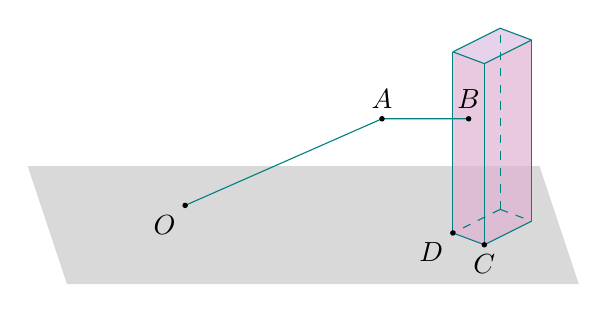
\begin{tikzpicture}[
				scale=1, 
				dot/.style={circle,fill,inner  sep=1.5pt}]
			 \path[fill=gray!30] (-4,-0.5) -- (2.5,-0.5) -- (2,1) -- (-4.5,1) -- cycle;
			 \coordinate (C) at (1.3,0);
			 \coordinate (D) at (0.9,0.15);
			\coordinate  (C_back) at (1.9,0.3);
			 \coordinate (D_back) at (1.5,0.45);
			 \coordinate (C_top) at (1.3,2.3);
			\coordinate (D_top)  at (0.9,2.45);
			\coordinate (C_back_top) at  (1.9,2.6);
			\coordinate (D_back_top) at  (1.5,2.75);
			\fill[purple!80!blue!30,opacity=0.7] (C) -- (C_back) -- (C_back_top) --  (C_top) -- cycle;
			\fill[purple!80!blue!30,opacity=0.7] (D) -- (C)  -- (C_top) -- (D_top) -- cycle;
			\fill[purple!60!blue!25,opacity=0.7] (D_top) -- (C_top) -- (C_back_top) -- (D_back_top) --  cycle;
			\draw[teal,dashed] (D_back) -- (D); 
			 \draw[teal,dashed] (D_back) -- (C_back);
			 \draw[teal,dashed] (D_back) -- (D_back_top);
			 \draw[teal] (D) -- (C);
			\draw[teal]  (C) -- (C_back);
			\draw[teal] (C)  -- (C_top);
			\draw[teal] (D) -- (D_top); 
			\draw[teal] (C_back) --  (C_back_top);
			\draw[teal]  (C_top) -- (C_back_top);
			\draw[teal] (D_top)  -- (C_top);
			\draw[teal] (D_top) -- (D_back_top); 
			\draw[teal]  (C_back_top) -- (D_back_top);
			 \coordinate (B) at (1.1,1.6);
			\coordinate (A) at (0,1.6); 
			\coordinate (O) at  (-2.5,0.5);
			\draw[teal] (O) --  (A) -- (B);
			\fill (O) circle  (1pt) node[below left]{$O$};
			\fill (A) circle (1pt)  node[above]{$A$};
			\fill (B) circle (1pt)  node[above]{$B$};
			 \fill (C) circle (1pt) node[below]{$C$};
			\fill  (D) circle (1pt) node[below left]{$D$};
		\end{tikzpicture}
	 }\noindent
	Vị trí giao hàng là điểm $B$ nằm trên mặt phẳng $(P)$. Drone bắt đầu bay từ kho hàng tại gốc tọa độ $O(0;0;0)$. Ban đầu, nó bay theo một đường thẳng đến vị trí $A(30;40;120)$. Từ vị trí $A$, drone thay đổi đường bay, di chuyển theo phương vuông góc với mặt phẳng $(P)$ đến vị trí giao hàng  $B$. Tính khoảng cách từ $O$ đến $B$ (làm tròn đến hàng đơn vị).
	\shortans{126} 
	\loigiai{ 
		Ta có  $\overrightarrow{CD}=(20;-40;0)=20\overrightarrow{u}$ với $\overrightarrow{u}=(1;-2;0)$.\\
		Do $(P)$ là mặt phẳng thẳng đứng qua $C$ và $D$ nên nhận vec-tơ $\overrightarrow{u}=(1;-2;0)$ và $\overrightarrow{k}=(0;0;1)$ làm cặp vec-tơ chỉ phương nên vec-tơ pháp  tuyến của $(P)$ là $\overrightarrow{n}=\left[\overrightarrow{u},\overrightarrow{k}\right]=(-2;-1;0)$ hay $\overrightarrow{n}=(2;1;0)$.\\
		Phương trình mặt phẳng  $(P) \colon 2(x-10)+1(y-50)+0(z-0)=0 \Leftrightarrow 2x+y-70=0$.\\
		Đường thẳng $AB$  vuông góc với $(P)$ nên nhận vec-tơ pháp tuyến của $(P)$ làm vec-tơ chỉ phương $\overrightarrow{u}_{AB}=(2;1;0)$ nên có phương trình đường thẳng $AB \colon$ $\heva{&x=30+2t\\&y=40+t\\&z=120.}$\\
		Vì $B$ là giao điểm của đường thẳng $AB$ và mặt phẳng  $(P)$ nên ta có
		\allowdisplaybreaks 
		\begin{eqnarray*}
			&&2(30+2t)+(40+t)-70=0\\ 
			&\Leftrightarrow&5t+30=0 \\ 
			&\Leftrightarrow&5t=-30 \\ 
			 &\Leftrightarrow&t=-6.
		\end{eqnarray*}
		Từ đó suy ra  $B(18;34;120) \Rightarrow OB=\sqrt{18^2+34^2+120^2}=126$.
	 }
\end{bt}

% nguồn: Lop_12_Hinh_hoc_Chuong_2
\begin{bt}%[2H2V2-6]%[ma:681aa2f0]
	Cho ba lực $\overrightarrow{F}_1=\overrightarrow{MA}$, $\overrightarrow{F}_2=\overrightarrow{MB}$, $\overrightarrow{F}_3=\overrightarrow{MC}$ cùng tác động vào một ô tô tại điểm $M$ và ô tô đứng yên. Cho biết cường độ hai lực $\overrightarrow{F}_1$, $\overrightarrow{F}_2$ đều bằng $25$N và góc $\widehat{AMB}=60^\circ$. Khi đó tính cường độ $\overrightarrow{F}_3$ (làm tròn đến hàng phần chục). 
	\begin{center}
		\begin{tikzpicture}
				\def \c{3}  \def \g{30};
				\draw[-stealth] (0,0) coordinate  (A)
					--(-\g:\c)  coordinate (B)--++(0:\c) coordinate (C)
					(B)--++(\g-180:\c) coordinate  (D);
				\draw[-stealth]  (B)--(A);
				\draw[-stealth] (B)--(C); 
				\path  (B)--(A) node[pos=0.5,sloped,above]{$\vec{F_1}$}
					(B)--(C) node[pos=0.5,sloped,above]{$\vec{F_3}$} 
					 (B)--(D) node[pos=0.5,sloped,above]{$\vec{F_2}$};
				\foreach \x/\g/\d in {A/90/A,B/-90/M,C/-90/C,D/90/B} 
				 \fill (\x) circle (1pt)
					($(\x)+(\g:3mm)$) node{\d}; 
				\draw pic [draw,angle radius = 9mm,"$60^\circ$"]{angle = A--B--D}; 
			\end{tikzpicture}
	\end{center}
	\shortans{43,3} 
	\loigiai{ 
		\begin{center}
			\begin{tikzpicture}
					 \def \c{3} \def \g{30};
					\draw[-stealth] (0,0) coordinate (A) 
						--(-\g:\c) coordinate (B)--++(0:\c) coordinate  (C)
						 (B)--++(\g-180:\c) coordinate (D);
					\path ($(A)-(B)+(D)$) coordinate (E) 
						(B)--(A) node[pos=0.5,sloped,above]{$\vec{F_1}$} 
						 (B)--(C) node[pos=0.5,sloped,above]{$\vec{F_3}$}
						(B)--(D) node[pos=0.5,sloped,above]{$\vec{F_2}$} 
						(B)--(E)  node[pos=0.5,sloped,above]{$\vec{F_1}+\vec{F_2}$};
					\draw[-stealth]  (B)--(A);
					 \draw[-stealth] (B)--(C);
					\draw[-stealth] (B)--(E); 
					\draw[dashed] (A)--(E)--(D); 
					\foreach  \x/\g/\d in {A/90/A,B/-90/M,C/-90/C,D/90/B,E/90/D}
					 \fill (\x) circle (1pt)
						($(\x)+(\g:3mm)$) node{\d}; 
					\draw pic [draw,angle radius =  9mm,"$60^\circ$"]{angle = A--B--D};
				\end{tikzpicture}
		\end{center}
		Ta  có $\overrightarrow{F_1}+\overrightarrow{F_2}=\overrightarrow{MA}+\overrightarrow{MB}=\overrightarrow{MD}$ (với $D$ là điểm sao cho $AMBD$ là hình bình hành). \\
		Ta có  $MA=\left|\overrightarrow{MA}\right|=\left|\overrightarrow{F}_1\right|=25$N và $MB=\left|\overrightarrow{MB}\right|=\left|\overrightarrow{F}_2\right|=25$N. \\
		Do $\widehat{AMB}=60^\circ$ nên $\Delta  MAB$ là tam giác đều. \\Khi đó $MD=2\cdot \dfrac{25\sqrt{3}}{2}=25\sqrt{3}$ (N).\\
		Do ô tô đứng yên nên cường độ lực tác  dụng lên ô tô bằng $0$ hay $\overrightarrow{F}_1+\overrightarrow{F}_2+\overrightarrow{F}_3=\overrightarrow{0}$.\\
		 Suy ra
		 $\overrightarrow{F}_3=-(\overrightarrow{F}_1+\overrightarrow{F}_2)
		\Rightarrow \left|\overrightarrow{F}_3\right|=\left| -(\overrightarrow{F}_1+\overrightarrow{F}_2)\right| 
		=\left|\overrightarrow{DM}\right|=MD=25\sqrt{3}$  (N).\\
		Vậy cường độ của $\overrightarrow{F}_3$ là $25\sqrt{3}\approx 43{,}3$ (N). 
	} 
\end{bt}

% nguồn: Lop_12_Hinh_hoc_Chuong_2
\begin{bt}%[2H2V2-6]%[ma:7385dbfb]
	Nhân dịp lễ 30/04/2025, tại Quảng trường trung tâm TP. Hồ Chí Minh diễn ra màn trình diễn máy bay trực thăng kéo cờ Tổ quốc và cờ Đảng. Hai máy bay cất cánh cùng lúc từ một địa điểm. Sau một thời gian, chiếc thứ nhất cách điểm xuất phát $3$ km về phía Nam và $1$ km về phía Đông, đồng thời cách mặt đất $1$ km. Chiếc thứ hai nằm cách điểm xuất phát $2$ km về phía Bắc, $1$ km về phía Tây đồng  thời cách mặt đất $500$ m. Cùng thời điểm đó, một sĩ quan công an đứng trên mặt đất quan sát thấy hai chiếc máy bay nói trên. Biết rằng, so với các vị trí quan sát trên mặt đất, vị trí chiến sĩ công an đứng có tổng khoảng cách đến hai chiếc máy bay là nhỏ nhất. Khoảng cách từ vị trí chiến sĩ công an đứng quan sát đến điểm xuất phát của hai chiếc máy bay là bao nhiều kilomét (kết quả làm tròn đến hàng phần trăm).
	 \shortans{0,47}
	 \loigiai{
		\begin{center}
			\begin{tikzpicture}[>=stealth,line join=round,line cap=round,font=\footnotesize,scale=1]
					 \path
						(0:0)  coordinate (O)
						(0:3)  coordinate (A)
						 (180:3) coordinate (A')
						 (90:3) coordinate (B)
						(-145:2.5) coordinate  (C)
						(A)++(C)  coordinate (D)
						(D)++(B)  coordinate (E)
						($(O)!1.3!(A)$) coordinate  (y)
						($(O)!1.3!(A')$) coordinate  (y')
						($(O)!1.3!(B)$)  coordinate (z)
						($(O)!1.3!(C)$) coordinate (x) 
						($(C)!0.5!(D)$) node[below]{$3$ km} 
						($(A)!0.5!(D)$) node[below right]{$1$ km} 
						($(E)!0.3!(D)$)  node[right]{$1$ km};
					\draw[->] 
						(O)--(z); 
					 \draw[->]
						(O)--(y') node[above  right]{Bắc};
					\draw (O)--(y) node[right]{Nam}; 
					 \draw[->]
						(O)--(x) node[below]{Đông}; 
					\fill [scale=.1,yshift=20  cm,xshift=10 cm]
						(-1,0) rectangle (1,1) 
						(-1,2).. controls  +(135:1) and +(180:4).. (0,7)
						.. controls +(180:2) and +(135:2)..  (-.5,2)
						.. controls +(120:2) and +(180:1)..  (0,6.99)
						 .. controls +(0:1) and +(60:2).. (.5,2)
						..  controls +(45:2) and +(0:2).. (0,7)
						.. controls +(0:4)  and +(45:1).. (1,2);
					\draw[scale=.1,yshift=20 cm,xshift=10 cm]  (-1,0) rectangle (1,2)
						(0,1)--(0,2);; 
					\draw[dashed] 
						 (A)--(D)--(C)
						(D)--(E)--(B); 
					\foreach \x/\g in {x/0,y/90,z/180}\fill (\x)+(\g:3mm) node{$ \x $}; 
					\foreach \x/\g in {O/-90}\fill (\x) circle (1pt)+(\g:3mm) node{$  \x $};
					\foreach  \x/\g in {E/0}\fill (\x) circle (1pt);
				\end{tikzpicture}
		\end{center}
		Xét hệ trục tọa  độ $Oxyz$ với điểm xuất phát của hai chiếc máy bay là gốc tọa độ $O(0; 0; 0)$, trục $Ox$: hướng đông, trục $Oy$ hướng Bắc, trục $Oz$ hướng lên trên và mặt đất là mặt phẳng $Oxy$.\\
		Đơn vị trên  mỗi trục là $1$ km.\\
		Sau một thời gian máy bay thứ nhất cách điểm xuất phát $3$ km về phía Nam và $1$ km về phía Đông, cách  mặt đất $1$ km nên tọa độ của máy bay thứ nhất là $A (1; -3; 1)$.\\
		Máy bay thứ hai nằm cách điểm xuất phát $2$ km về phía Bắc, $1$ km về phía Tây đồng thời cách mặt đất $500$ m nên  có tọa độ là $B (-1; 2; 0{,}5)$.\\
		Gọi $C$ là điểm đối xứng với $A$ qua mặt phẳng $(Oxy)$.\\ 
		Ta có  $C(1; -3; -1)$.\\
		Do chiến sĩ công an đứng trên mặt đất  nên giả sử vị trí của chiến sĩ có tọa độ $P(x; y; 0)$.\\
		Ta có  $PA+PB=PC+PB\ge BC$. Dấu bằng xảy ra khi và chỉ khi $P, B, C$ thẳng hàng.\\
		Ta có $\overrightarrow{BC}=(2; -5; -1{,}5)$ và $\overrightarrow{BP}=(x+1; y-2; -0{,}5)$.\\ 
		Do $P, B, C$ thẳng hàng nên ta có 
		\begin{align*}
			 \dfrac{x+1}{2}=\dfrac{y-2}{-5}=\dfrac{-0{,}5}{-1{,}5}\Rightarrow\heva{&x=-\dfrac{1}{3}\\&y=\dfrac{1}{3}.}
		\end{align*}
		Khi đó $P\left(-\dfrac{1}{3}; \dfrac{1}{3}; 0\right)\Rightarrow  OP=\sqrt{\left(-\dfrac{1}{3}\right)^2+\left(\dfrac{1}{3}\right)^2+0^2}=\dfrac{\sqrt{2}}{3}\approx0{,}47$.
	 }
\end{bt}

% nguồn: Lop_12_Hinh_hoc_Chuong_2
\begin{bt}%[2H2V2-6]%[ma:ea073f9c]
	Cho biết bốn đoạn thẳng nối từ một đỉnh của tứ diện đến trọng tâm mặt đối diện luôn cắt nhau  tại một điểm gọi là trọng tâm của tứ diện đó. Một phân tử metan $\mathrm{CH}_{4}$ được cấu tạo bởi bốn nguyên tử hydrogen ở các đỉnh của một tứ diện đều và một nguyên tử carbon ở trọng tâm của tứ diện. Góc liên kết là góc tạo bởi liên kết $H-C-H$ là góc giữa các đường nối nguyên tử carbon với hai trong số các nguyên tử hydrogen. Tính số đo góc liên kết này (làm tròn kết quả đến hàng đơn vị của độ).\\
	\shortans{109} 
	 \loigiai{
		\begin{center}
			\begin{tikzpicture}[line join=round,line cap=round,>=stealth,scale=0.6,font=\footnotesize]
					\foreach \x/\y/\n in  {0/0/A,6/0/C,2/-2/B} \coordinate (\n) at (\x,\y);
					\coordinate (S)  at ($(A)+(0,4)$);
					\coordinate (M) at ($(B)!1/2!(C)$); 
					\coordinate (G) at  ($(A)!2/3!(M)$);
					\draw  (S)--(A)--(B)--(C)--(S)--(B);
					 \draw[dashed] (A)--(C)
						 (A)--(M);
					\foreach  \t/\g in {A/180,B/-110,C/0,S/90,M/-40,G/-90}{
						\fill (\t)  circle (1pt) node[shift={(\g:8pt)}]{$ \t $};
					} 
					\draw pic[thin,draw,angle  radius=2mm] {right angle= A--B--C};
				\end{tikzpicture}4
			4 
		\end{center}
		Xét  tứ diện $ABCD$ có $G$ là trọng tâm thì $\overrightarrow{GA}+\overrightarrow{GC}+\overrightarrow{GC}+\overrightarrow{GD}=\overrightarrow{0}$ và $GA = GB = GC=x$.\\
		Ta có: $-\overrightarrow{GA}=\overrightarrow{GC}+\overrightarrow{GC}+\overrightarrow{GD}$, bình phương hai vế ta  được
		\begin{eqnarray*}
			&&GA^2 = GB^2 + GC^2+ GD^2 + 2 \overrightarrow{GB} \cdot \overrightarrow{GC}+2 \overrightarrow{GB} \cdot \overrightarrow{GD}+2  \overrightarrow{GC} \cdot \overrightarrow{GD} \\
			&\Leftrightarrow& x^{2}=3 x^{2}+2 x^{2} \cos \alpha+2 x^{2} \cos \alpha+2  x^{2} \cos \alpha\\
			&\Leftrightarrow& -2 x^{2}=6 x^{2} \cdot \cos  \alpha\\
			&\Rightarrow& \cos \alpha=\dfrac{-1}{3}\\ 
			 &\Rightarrow& \alpha \approx 109^{\circ}.
		\end{eqnarray*}
		Vậy số  đo liên kết này là $109^{\circ}$
	 }
\end{bt}

% nguồn: Lop_12_Hinh_hoc_Chuong_2
\begin{bt}%[2H2V2-6]%[ma:6481637e]
	Trong một trung tâm logistics, người ta cần thiết kế một thùng hàng  hình chữ nhật để đóng gói và vận chuyển thiết bị điện tử. Tổng diện tích các mặt ngoài của thùng bằng $36$ m$^{2}$ (bao gồm cả mặt đáy, mặt nắp và $4$ mặt bên). Để đảm bảo khả năng đóng gói vừa vặn thiết bị, đường chéo không gian của thùng phải dài $6$ mét. Thể tích lớn nhất có thể của thùng hàng này là bao nhiêu (tính theo đơn vị mét khối, làm tròn đến hàng phần chục)?
	 \shortans{11,3}
	 \loigiai{
		\begin{center}
			\begin{tikzpicture}[scale=1,font=\footnotesize,line join=round,line cap=round,>=stealth]
					\def\bc{4} 
					 \def\ba{2}
					 \def\gocB{35}
					\coordinate[label=below right:$D'$] (B) at (0,0); 
					 \coordinate (C) at (\gocB:\ba);
					\coordinate[label=below:$C'$] (A) at  (\bc,0);
					\coordinate[label=below right:$B'$] (D) at ($(C)-(B)+(A)$); 
					\coordinate[label=above  left:$C$] (A') at ($(A)+(90:\bc)$);
					\coordinate[label=left:$D$] (B') at  ($(B)-(A)+(A')$);
					\coordinate[label=below right:$A$] (C') at  ($(C)-(A)+(A')$);
					 \coordinate[label=right:$B$] (D') at ($(D)-(A)+(A')$);
					\draw[teal]  (B')--(B)
						 (D)--(D')--(A')--(B')--(C')--(D')
						(B)--(A)--(D) 
						(A)--(A'); 
					\draw[teal,dashed]  (C)--(B)
						(C)--(D) 
						 (C)--(C');
					\foreach  \diem in {A,B,C,D,A',B',C',D'} \fill (\diem) circle (1.0pt);
					\draw[-stealth] (D)--+(0:1) node[right]{$y$}; 
					\draw[-stealth] (C')--+(90:1)  node[above]{$z$};
					\draw[-stealth] (B)--+(-145:.75) node[below]{$x$}; 
					\draw[-stealth,blue] (C)--+(0:.8) node[above]{$\vec{j}$}; 
					\draw[-stealth,blue] (C)--+(90:.85)  node[above left]{$\vec{k}$};
					 \draw[-stealth,blue] (C)--+(-145:.65) node[above]{$\vec{i}$};
					\fill (C) circle (1pt) node[below right]{$A'\equiv O$}; 
					\draw[teal,dashed][->](C)--(A'); 
				\end{tikzpicture}
		\end{center}
		\begin{enumerate}[Cách 1.]
			\item Gọi $x$, $y$, $z$ lần lượt là  độ dài của các cạnh $AB$, $AD$, $AA'$\\
			Diện tích tất cả các  mặt là
			\begin{align}
				S_{tp}=2(xy+yz+xz)=36 \Leftrightarrow xy+yz+xz=18. \tag{1}\label{12D1-1-1} 
			\end{align}
			Độ dài đường chéo $AC'=\sqrt{x^{2}+y^{2}+z^{2}}=6 \Leftrightarrow x^{2}+y^{2}+z^{2}=36 $.\\ 
			Suy ra \begin{align}
			\left( x^{2}+y^{2}+z^{2}\right)  =x^{2}+y^{2}+z^{2}+2(xy+yz+xz)=72 \Leftrightarrow x+y+z=6\sqrt{2} \tag{2}\label{12D1-1-2}.
		\end{align}
		Từ $\eqref{12D1-1-1}$ ta có $y+z=6\sqrt{2}-x$.\\ 
		Do đó,  kết hợp với $\eqref{12D1-1-2}$ ta được
		\begin{align}
			yz=18-x(y+z)=18-x(6\sqrt{2}-x)=x^{2}-6\sqrt{2}x+18 \nonumber. 
		\end{align}
		Ta luôn có $(y+z)^{2} \geq 4yz$, $\forall y$,  $z$ nên
		\begin{eqnarray*}
			&&\left( 6\sqrt{2}-x\right)  ^{2} \geq 4\left( x^{2}-6\sqrt{2}x+18\right) \\
			&\Leftrightarrow&  3x^{2}-12\sqrt{2}x \leq 0 \\
			&\Leftrightarrow&0\leq x\leq  4\sqrt{2}.
		\end{eqnarray*}
		Thể tích của khối hộp chữ nhật là $V=xyz=x\left( x^{2}-6\sqrt{2}+18\right) =x^{3}-6\sqrt{2}x^{2}+18x$.\\ 
		Bài toán trở thành tìm giá trị lớn nhất  của hàm số $f(x)=x^{3}-6\sqrt{2}x^{2}+18x$ trên đoạn $[0;4\sqrt{2}]$.\\
		Ta có $f'(x)=3x^{2}-12\sqrt{2}x+18$ và $f'(x)=0  \Leftrightarrow \hoac{&x=\sqrt{2} \in [0;4\sqrt{2}]\\
		 &3\sqrt{2} \in [0;4\sqrt{2}] }$.\\
		Ta tính được  $f(0)=0$; $f\left( 4\sqrt{2}\right) =8\sqrt{2}$; $f\left( \sqrt{2}\right) =8\sqrt{2}$; $f\left( 3\sqrt{2}\right) =0$.\\
		 Với $x=\sqrt{2}$ thì $\heva{&y+z=5\sqrt{2}\\
		&yz=8.  }$\\
		Như thế $(x;y;z)  \in \left\lbrace \left( \sqrt{2};4\sqrt{2};\sqrt{2}\right) ,\left( \sqrt{2};\sqrt{2};4\sqrt{2}\right) \right\rbrace. $\\
		 Với $x=4\sqrt{2}$ thì $\heva{&y+z=2\sqrt{2}\\
		&yz=2. }$\\ 
		Như  thế $(x;y;z)=\left( 4\sqrt{2};\sqrt{2};\sqrt{2}\right) $.\\
		Vậy thể tích của khối  hộp chữ nhật lớn nhất là
		 $8\sqrt{2}\approx 11,3$ m$^{3}$ khi $(x;y;z)=\left( \sqrt{2};4\sqrt{2};\sqrt{2}\right) $ và hoán vị của nó.
		\item Gọi $x$, $y$, $z$ lần lượt là độ dài của các cạnh $AB$,  $AD$, $AA'$.\\
		 Diện tích tất cả các mặt là
		\begin{align}
			S_{tp}=2(xy+yz+zx)=36 \Leftrightarrow  xy+yz+xz=18 \tag{1} \label{12D1-1-3}
		\end{align}
		Độ dài đường chéo $AC=\sqrt{x^{2}+y^{2}+z^{2}}=6 \Leftrightarrow x^{2}+y^{2}+z^{2}=36$\\ 
		 Suy ra
		\begin{align}
			(x+y+z)^2 =x^{2}+y^{2}+z^{2}+2(xy+yz+xz)=72 \Leftrightarrow x+y+z  =6\sqrt{2} \tag{2}\label{12D1-1-4}
		\end{align}
		Thể tích của  khối hộp chữ nhật
		\begin{align}
			 V=xyz \tag{3}\label{12D1-1-5}
		\end{align}
		Từ $\eqref{12D1-1-3}$, $\eqref{12D1-1-4}$, $\eqref{12D1-1-5}$ suy ra $x$, $y$, $z$ là $3$ nghiệm của phương  trình
		\begin{align}
			 X^{3}-6\sqrt{2}X^{2}+18X-V=0 \nonumber \\
			\Leftrightarrow V= X^{3}-6\sqrt{2}X^{2}+18X. \tag{4} \label{12D1-1-6} 
		\end{align}
		Bảng biến thiên của hàm số $f(x)=X^{3}-6\sqrt{2}X^{2}+18X $ trên $\left( 0;6\sqrt{2}\right) $  như sau:
		\begin{center}
			
\begin{tikzpicture}
					 \tkzTabInit[espcl=3,lgt=1.5,nocadre]
						{$x$/0.9,$y'$/0.7,$y$/2.5} 
						 {$0$,$\sqrt{2}$,$3\sqrt{2}$,$6\sqrt{2}$}
					 \tkzTabLine{,+,0,-,0,+,}
					 \tkzTabVar{-/$0$,+/$8\sqrt{2}$,-/$0$,+/$108\sqrt{2}$}
				\end{tikzpicture}
		\end{center}
		Dựa vào bảng biến thiên, giá trị lớn nhất của $V$ để phương trình $\eqref{12D1-1-6}$ có $3$ nghiệm (không cần phân biệt) trên khoảng $\left( 0;6\sqrt{2}\right) $ là $8\sqrt{2}$. 
		Vậy thể tích của khối hộp chữ nhật lớn nhất là 
		$8\sqrt{2}\approx 11{,}3 $ m$^{3}$  khi $(x;y;z)=\left( \sqrt{2};4\sqrt{2};\sqrt{2}\right) $ và các hoán vị của nó.
	\end{enumerate}
} 
\end{bt}

% nguồn: Lop_12_Hinh_hoc_Chuong_2
\begin{bt}%[2H2V2-6]%[ma:d99caa73]
	Một toà nhà được thiết kế để làm 2 phòng dạy học có trang bị máy chiếu. Mái nhà là dạng mái vát $CDFE$ như hình vẽ. Chiều dài của mỗi phòng học là $OA=30$ m và chiều rộng là $OB=20$ m, chiều cao các bức tường $BD=10$ m và $EA=6$ m. Từ vị trí $P$ cách $B$ một khoảng $10$ m, người ta xây các bậc thang cao dần về phía cuối của  phòng học để đặt các dãy bàn ghế học sinh trên các bậc thang đó. Chiều rộng mỗi bậc thang là $2$ m và chiều cao mỗi bậc thang là $20$ cm.
	\begin{center}
		\begin{center}
			\begin{tikzpicture}[scale=0.4,line cap=round,line join=round,semithick,
						declare function={a=12;  b=8; c=8; d=6;}]
					\begin{scope}[x={(0.4cm,-0.3cm)},y={(1cm,0cm)},z={(0,1cm)},transform shape]
						 \draw (0,0,0)--(a,0,0) coordinate (B)
						(0,-b,0) coordinate (A)  --(0,b,0);
						\draw  (0,0,0) coordinate (O) --(0,0,c) coordinate (C)
						(a,0,0)--(a,0,c) coordinate  (D)
						(a,-b,0) coordinate (G)--+(0,0,d) coordinate  (F)
						(a,b,0)--+(0,0,d) 
						 (0,-b,0)--+(0,0,d) coordinate (E)
						(0,b,0)--+(0,0,d); 
						\draw[line width =  1pt] (A) -- (a,-b,0)--(a,b,0)--(0,b,0)--cycle;
						 \def\vien{($(C)!0.3!(B)$) -- ($(O)!0.3!(D)$)--($(C)!0.7!(B)$) -- ($(O)!0.7!(D)$)--cycle;}
						\path[fill=green!65!black]  \vien;
						\begin{scope}
						\clip  \vien;
						\foreach  \i in {0,0.2,...,12}{
						 \draw[gray!50,thin] (\i,0,0)--+(0,0,c);
						 \draw[gray!50,thin] (0,0,\i)--+(c,0,0);
						 }
						\end{scope}
						\draw[line  width = 1pt,color=gray!80!white] \vien;
						 \path
						(intersection of  E--D and F--C) coordinate (I)
						($(I)+(0,0,-2)$) coordinate  (Id)
						 (0.5*a,0,0.6*c) coordinate (K)
						 ($(A)!0.4!(E)$) coordinate (S)
						($(G)!0.4!(F)$)  coordinate (Q)
						($(S)!0.5!(Q)$) coordinate (X) 
						($(B)!0.3!(G)$) coordinate (P); 
						\draw[dashed] (I) |-  (K);
						 \draw (E)--(D)--(C)--(F);
						\fill[brown,fill  opacity=0.3,draw,black] (0,-b,d)--(0,0,c)--(0,b,d)--(a,b,d)--(a,0,c)--(a,-b,d)--cycle;
						\def\cao{0.3} 
						\def\dai{0.65} 
						 \def\sobac{8}
						\foreach \i in  {1,...,\sobac}{
						 \draw (a,{-b+(\i-1)*\dai},{(\sobac-\i+1)*\cao})--++(0,\dai,0)--+(0,0,-\cao);
						\draw[dashed] (0,{-b+(\i-1)*\dai},{(\sobac-\i+1)*\cao})--++(0,\dai,0)--+(0,0,-\cao); 
						 \draw (a,{-b+(\i)*\dai},{(\sobac-\i+1)*\cao})--(0,{-b+(\i)*\dai},{(\sobac-\i+1)*\cao});
						} 
						\draw  (a,-b,{(\sobac)*\cao})--(0,-b,{(\sobac)*\cao});
					\end{scope}
					\foreach \t/\g in {B/-90,A/-90,O/-90,C/90,D/90,E/90,F/90,I/90,Q/180,S/-170,X/180,P/-90}{ 
						\fill (\t)  circle (1pt) node[shift={(\g:12pt)}]{$\t$};
					} 
				\end{tikzpicture}
		\end{center}
	\end{center}
	Chủ toà nhà muốn lắp giá treo máy chiếu tại vị trí $I$ là giao của $DE$ và $CF$ như hình vẽ, vuông góc với mặt sàn sao cho không vướng vào đầu học sinh khi học sinh đó đứng tại bậc thang  ngay dưới máy chiếu (chiều cao học sinh đó là $1{,}8$ m) và cũng không che khuất tầm nhìn của học sinh ngồi ở hàng ghế sau cùng, tại vị trí $X$ trung điểm $SQ$, theo phương vuông góc bức tường $OBDC$ (chiều cao mắt học sinh so với bậc thang tại đó là $1{,}2$ m). Hỏi tổng độ dài thanh treo máy chiếu và cả thân máy chiếu lớn nhất là bao nhiêu mét? Kết quả làm tròn đến hàng phần mười.
	\shortans{4,8} 
	 \loigiai{
		Xét hệ trục tọa độ $Oxyz$ với $O$ là gốc tọa độ, các điểm $A \in Ox, B \in Oy, C \in Oz$ có tung độ, hoành độ và cao độ không  âm.\\
		Khi đó $A(30;0;0),  B(0;20;0), D(0;20;10); E(30;0;6)$.\\
		 $I(15;10;8)$ là trung điểm $DE$ nên hình chiếu của điểm $I$ trên sàn là $T(15;10;0)$.\\
		Gọi  $V$ là hình chiếu của $T$ trên đường thẳng $BP$, suy ra tọa độ điểm $V(15;20;0)$. Suy ra $V$ cách $P$ một khoảng bằng $5$ m.\\
		Tức là bậc thang  tại vị trí $U$ đang là bậc thang thứ 3, có chiều cao $60$ cm so với mặt sàn.\\
		Suy ra tọa độ điểm $U(15;10;0,6)$.\\ 
		Từ đó tọa độ đỉnh đầu học sinh đứng là $K(15;10;2{,}4)$. Khoảng cách $IK =  8-2{,}4=5{,}6m$. (1)\\
		Mặt  khác tọa độ điểm $X(30;10;2)$ nên tọa độ mắt học sinh ngồi tại $X$ là điểm $Z(30;10;3{,}2)$.\\
		Suy ra hiệu khoảng cách từ điểm $I$  đến sàn và từ điểm $Z$ đến sàn nhà là $8-3,2=4{,}8$ m (2).\\
		Điều (1) và (2) cho thấy tổng độ dài của thanh treo và  thân máy chiếu không quá $4,8$ mét để thoả mãn đồng thời cả 2 điều kiện.
	 }
\end{bt}

% nguồn: Lop_12_Hinh_hoc_Chuong_2
\begin{bt}%[2H2V2-6]%[ma:cd62b8a3]
	Thiên thạch với kích thước chỉ $30$ cm đến $40$ cm đến từ vùng không gian giữa các hành tinh, khi xuyên vào khí quyển Trái Đất ở độ cao $150$ km so với mực nước biển, tạo ra vùng không khí bốc cháy quanh nó rộng vài trăm mét gây nên hiện tượng sao băng. Xem Trái Đất là khối cầu có bán kính $6\,400$ km. Chọn hệ trục tọa  độ $Oxyz$ trong không gian có gốc $O$ tại tâm Trái Đất và đơn vị độ dài trên mỗi trục tọa độ là $1\,000$ km. Một thiên thạch (coi như một hạt) được phát hiện ở vị trí điểm $M\left(4{,}29;7;0\right)$ và đang chuyển động thẳng với tốc độ không đổi $960$ km/phút đến tâm Trái Đất. Xác định thời điểm (đơn vị phút) thiên thạch bị bốc cháy kể từ lúc phát hiện (làm tròn kết quả đến hàng phần trăm).
	 \shortans{1,73}
	 \loigiai{
	\immini{Thiên thạch được phát hiện ở  vị trí điểm $M$.\\
		Gọi khối cầu tâm $O$, bán kính $OC$ là Trái đất, với $O$  là tâm Trái đất.\\
		Phần vành khăn bên ngoài  là tầng khí quyển Trái đất.\\
		Ta có $1$ đơn vị $=1\,000$ km suy ra $6\,400$ km  $=6{,}4$ (đơn vị).\\\
		$M\left(4{,}29;7;0\right)\Rightarrow OM=\sqrt{\left(4{,}29\right)^{2}+7^{2}+0^{2}}=8{,}21$ (đơn  vị).\\
		$CD=150$ (km)  $\Rightarrow CD=0{,}15$ (đơn vị).\\
		$\Rightarrow DM=OM-OD=8{,}21-6{,}4-0{,}15=1{,}66$ (đơn  vị).\\
		 Theo thực tế $DM=1\,660$ km.
		}{\begin{tikzpicture}[scale=.5,>=stealth,line join=round,line cap=round,font=\footnotesize]
		 \def\a{3}
		\def\b{0.75} 
		\path (0,0)  coordinate (O)
			+(40:{\a}) coordinate  (C)
			+(40:{\a+\b}) coordinate  (D)
			($(O)!2!(D)$) coordinate  (M);
		 \draw[teal] (O) circle (\a);
		\draw[teal] (O) circle ({\a+\b}); 
		\draw[teal,smooth] (O)--(M); 
		\foreach \t/\g  in {O/90,C/90,D/90,M/90}{
			\draw[teal,fill=white] (\t) circle (1pt)  node[shift={(\g:9pt)},font=\scriptsize]{$\t$};
		} 
	\end{tikzpicture}
		 }
		\noindent Thời điểm  thiên thạch bị bốc cháy kể từ lúc phát hiện là
		$t=\dfrac{DM}{v}=\dfrac{1\,660}{960}\approx 1{,}73$ (phút). 
	} 
\end{bt}

% nguồn: Lop_12_Hinh_hoc_Chuong_2
\begin{bt}%[2H2V2-6]%[ma:a66147bd]
	Trong không gian $Oxyz$ (mỗi đơn~vị trên trục tọa độ dài $1~\mathrm{cm}$)  được đặt một góc trong một căn phòng. Có một cây quạt trần có ba cánh quạt và mỗi cánh cách đều nhau (minh họa như hình vẽ bên). Gọi $A(-10;-15;300)$ và $B(12;20;300)$ là hai trong ba đỉnh của cánh quạt trần. Chiều cao của ống treo với hộp điện cánh quạt gắn vào trần nhà là 50 cm và đỉnh $S(a;b;c)$ với $a > 0$ là giao điểm giữa trần nhà và ống treo cánh quạt. Tính $T=a-b+c$. (Kết quả làm tròn đến hàng đơn~vị).
	 \shortans{365}
	 \loigiai{
	\immini{Vì $SI\perp (ABC)$  nên $z_S=300+50=350$ nên $S(a;b;350)$ và $I(a;b;300)$.\\
		Do ba cánh quạt cùng nằm trên một mặt phẳng $z=300$ nên ta chỉ xét các yếu tố trên cùng mặt phẳng tọa độ (bỏ qua yếu tố  cao độ).\\
		 Gọi $K$ là trung điểm của $AB$ thì $K\left(1;\dfrac{5}{2}\right)$ và $\vec{AB}=(22;35)$.\\
		Véc-tơ $\vec{KI}\parallel (35;-22)$  nên $\vec{KI}=k(35;-22)$ mà $KI=AK\cdot \cot{60}^{\circ}=\dfrac{AK}{\sqrt{3}}=\sqrt{\dfrac{1709}{12}}$.}
		{\begin{tikzpicture}[scale=0.8,font=\footnotesize,line join=round,line cap=round,>=stealth]
		 \path
			(0,0)  coordinate (A)
			 ++(-60:2) coordinate (B)
			(4,0) coordinate (C) 
			($(B)!1/2!(A)$) coordinate  (K)
			($(C)!2/3!(K)$)  coordinate (I)
			($(I)+(0,3)$) coordinate  (S);
		\foreach  \i in{B,C,A}{\draw (S)--(\i);};
		\draw (A)--(B)--(C); 
		\draw[dashed]  (A)--(C)
			 (S)--(I)
			 (C)--(K)
			(A)--(I)--(B); 
		\foreach \i/\g in  {A/90,B/-120,C/-90,K/180,S/90,I/-60}
		\fill  (\i) circle (1pt)+(\g:4mm) node[scale=1]{$\i$};
	\end{tikzpicture}
		} 
		Do vậy  $\left|k(35;-22)\right|=\sqrt{\dfrac{1709}{12}}\Leftrightarrow|k|=\dfrac{\sqrt{\dfrac{1709}{12}}}{\sqrt{{35}^2+(-22)^2}}=\dfrac{1}{\sqrt{12}}\Rightarrow k=\pm \dfrac{1}{\sqrt{12}}$.\\
		Ta có $\begin{cases}
		 x_I=a=x_K+35k \\ y_I=b=y_K-22k
	\end{cases}\Leftrightarrow \begin{cases}
	 a=1+35k \\ b=2-22k.
	\end{cases}
	 $\\
	Mà do $a > 0\Leftrightarrow 1+35k > 0\Leftrightarrow k  >-\dfrac{1}{35}\Rightarrow k=\dfrac{1}{\sqrt{12}}$.\\
	Từ đó $\begin{cases}
	a=1+35k \\  b=2-22k
	\end{cases}
	 \Leftrightarrow
	\begin{cases}
		a=1+\dfrac{35}{\sqrt{12}} \\ b=2-\dfrac{22}{\sqrt{12}} \\  c=350.
	\end{cases}
	 $\\
	 Vậy
	\[T=a-b+c=\left(1+\dfrac{35}{\sqrt{12}}\right)-\left(2-\dfrac{22}{\sqrt{12}}\right)+350\approx  365.\]
} 
\end{bt}

% nguồn: Lop_12_Hinh_hoc_Chuong_2
\begin{bt}%[2H2V2-6]%[ma:970520de]
	\immini{ 
	Trong không gian với hệ trục tọa độ $Oxyz$,  một tấm bảng đồng chất có dạng hình vuông $ABCD$ tâm $H$ được treo nghiêng bởi bốn sợi dây $IA$, $IB$, $IC$, $ID$ gắn cố định tại điểm $I (0; 0; 9)$ như hình vẽ. Điểm $H (0; 0; 5)$, điểm $A (-\sqrt{2}; \sqrt{2}; 5)$ và góc $\widehat{HID}$ đạt giá trị nhỏ nhất. Gọi $\overrightarrow{F}_1$; $\overrightarrow{F}_2$; $\overrightarrow{F}_3$; $\overrightarrow{F}_4$ lần lượt là lực căng của các sợi dây $IB$; $IC$; $ID$; $IA$. Biết rằng $\left|\overrightarrow{F}_1\right|=50$ N và $\left|\overrightarrow{F}_2\right|=40$ N.
	Tính khối lượng $m$ (kg) của tấm bảng  (kết quả làm tròn đến hàng đơn vị) (Cho gia tốc trọng trường $g=9{,}8 \mathrm{m/s^2}$ và trọng lượng của tấm bảng được tính theo công thức $P=m\cdot g$).}{
	\begin{tikzpicture}[line join=round,line cap=round,font=\footnotesize,scale=1,>=stealth]
			 \def \r{3}
			\path 
				(0,0) coordinate (B) 
				(0:\r)  coordinate (D)
				(-50:0.5*\r) coordinate  (C)
				($(C)!0.5!(D)$) coordinate  (M)
				($(B)!2/3!(M)$) coordinate  (G_0)
				($(B)!(G_0)!(D)$)  coordinate (X)
				($(X)!1.1!90:(D)$) coordinate  (A)
				($(A)!0.6!(G_0)$) coordinate (G); 
			 \draw (A)--(B)--(C)--(D)--(A)--(C);
			\draw[dashed]  (B)--(D)
				(A)--(G_0) 
				(G)--(B)--(M); 
			\foreach  \x/\g in {A/90,B/180,C/-90,D/0,M/-30,G_0/-90,G/0}\fill (\x) circle (1pt)+(\g:.3) node{$\x$};
		\end{tikzpicture}2
	2 
	 }
	 \shortans{15}
	\loigiai{ 
	Do  $H$ là trung điểm của $AC$ nên $C \left(\sqrt{2}; -\sqrt{2}; 5\right)$ và gọi $D (a; b; c)$.\\
	Khi đó $\overrightarrow{HD}=(a; b; c-5)$; $\overrightarrow{AC}=\left(2\sqrt{2};  -2\sqrt{2}; 0\right)$.\\
	Mà $\overrightarrow{HD}\perp\overrightarrow{AC}$  nên suy ra $2\sqrt{2}a-2\sqrt{2}b+0\cdot(c-5)=0\Leftrightarrow 2\sqrt{2}a=2\sqrt{2}b\Leftrightarrow a=b$.\\
	 Suy ra $\overrightarrow{CD}=\left(a-\sqrt{2}; a+\sqrt{2}; c-5\right)$; $\overrightarrow{AD}=\left(a+\sqrt{2}; a-\sqrt{2}; c-5\right)$.\\
	Mà  $\overrightarrow{CD}\perp\overrightarrow{AD}\Rightarrow c=\sqrt{4-2a^2}+5$.\\
	Ta có $\overrightarrow{ID}=\left(a; a; \sqrt{4-2a^2}-4\right)$; $\overrightarrow{IH}=(0; 0;  -4)$.\\
	Khi  đó $\cos{\widehat{HID}}=\dfrac{16-4\sqrt{4-2a^2}}{4\sqrt{a^2+a^2+\left(\sqrt{4-2a^2}-4\right)^2}}=\dfrac{4-\sqrt{4-2a^2}}{\sqrt{20-8\sqrt{4-2a^2}}}$.\\
	Khảo sát hàm số $f(a)=\dfrac{4-\sqrt{4-2a^2}}{\sqrt{20-8\sqrt{4-2a^2}}}$, tìm được giá trị  nhỏ nhất của $f(a)$ bằng $\dfrac{\sqrt{3}}{2}$ khi $a=\dfrac{\sqrt{6}}{2}$.\\
	Khi đó $A=\left(-\sqrt{2}; \sqrt{2}; 5\right)$; $B=\left(-\dfrac{\sqrt{6}}{2};-\dfrac{\sqrt{6}}{2}; 4\right)$; $C=\left(\sqrt{2}; -\sqrt{2};  5\right)$; $D=\left(\dfrac{\sqrt{6}}{2}; \dfrac{\sqrt{6}}{2}; 6\right)$.\\
	Ta có $\overrightarrow{IA}=\left(-\sqrt{2}; \sqrt{2}; -4\right)\Rightarrow  \left|\overrightarrow{IA}\right|=2\sqrt{5}$; $\overrightarrow{IC}=\left(\sqrt{2}; -\sqrt{2}; -4\right)\Rightarrow \left|\overrightarrow{IC}\right|=2\sqrt{5}$.\\
	Khi  đó $\left|\overrightarrow{F}_4\right|=\left|\overrightarrow{F}_2\right|=k\cdot2\sqrt{5}=40\Rightarrow k=4\sqrt{5}$.\\
	Suy ra $\overrightarrow{F}_2=\left(-4\sqrt{10}; 4\sqrt{10};  -16\sqrt{5}\right)$; $\overrightarrow{F}_4=\left(4\sqrt{10}; -4\sqrt{10}; -16\sqrt{5}\right)$.\\
	 Tương tự $\overrightarrow{IB}=\left(-\dfrac{\sqrt{6}}{2}; \dfrac{\sqrt{6}}{2}; -5\right)\Rightarrow \left|\overrightarrow{IB}\right|=2\sqrt{7}$; $\overrightarrow{ID}=\left(\dfrac{\sqrt{6}}{2}; \dfrac{\sqrt{6}}{2}; -3\right)\Rightarrow \left|\overrightarrow{ID}\right|=2\sqrt{3}$.\\
	Sử dụng tỉ lệ giữa  độ dài dây và độ lớn lực, ta có $\dfrac{\left|\overrightarrow{F}_1\right|}{\left|\overrightarrow{F}_2|\right|}=\dfrac{2\sqrt{7}}{2\sqrt{3}}\Rightarrow \left|\overrightarrow{F}_3\right|=\dfrac{50\sqrt{21}}{7}$.\\
	Suy ra $\overrightarrow{F}_3=\left(\dfrac{25\sqrt{42}}{14}; -\dfrac{25\sqrt{42}}{14};  -\dfrac{75\sqrt{7}}{7}\right)$; $\overrightarrow{F}_1=\left(-\dfrac{25\sqrt{42}}{14}; -\dfrac{25\sqrt{42}}{14}; -\dfrac{125\sqrt{7}}{7}\right)$.\\
	Để hệ cân bằng thì $\overrightarrow{F}_1+\overrightarrow{F}_2+\overrightarrow{F}_3+\overrightarrow{F}_4=\overrightarrow{P}=\left(0; 0; -32\sqrt{5}-\dfrac{200\sqrt{7}}{7}\right)\Rightarrow  \left|P\right|=\dfrac{200\sqrt{7}}{7}+32\sqrt{5}$.\\
	Vậy khối lượng của tấm bảng là $m=\dfrac{P}{g}=\dfrac{\dfrac{200\sqrt{7}}{7}+32\sqrt{5}}{9{,}8}\approx15$  (kg).
	} 
\end{bt}

% nguồn: Lop_12_Hinh_hoc_Chuong_2
\begin{bt}%[2H2V2-6]%[ma:f8bc0d8d]
	Có ba lực cùng tác động vào một vật. Hai trong ba lực này hợp với nhau một góc $120^\circ$ và có độ  lớn lần lượt là $10$ N và $8$ N . Lực thứ ba vuông góc với mặt phẳng tạo bởi hai lực đã cho và có độ lớn $6$ N . Tính độ lớn của hợp lực của ba lực trên. (Làm tròn kết quả đến hàng đơn vị)
	\shortans{11} 
	\loigiai{ 
		Gọi $\overrightarrow{F}_{1}$, $\overrightarrow{F}_{2}$, $\overrightarrow{F}_{3}$ lần  lượt là ba lực tác động vào một vật đặt tại điểm $O$ như Hình.\\
		\begin{center}
			\begin{tikzpicture}[scale=1,font=\footnotesize,line join=round,line cap=round,>=stealth]
					 \def\x{2.5}
					\def\y{4} 
					\def\z{3} 
					\def\gocXY{-150} 
					\coordinate[label=above left:$O$]  (O) at (0,0);
					\coordinate (x)  at (\gocXY:\x);
					\coordinate (y)  at (\y,0);
					 \coordinate (z) at (0,\z);
					 \def\vtdv{1.7}
					\coordinate  (i) at (\gocXY:\vtdv);
					\coordinate  (j) at (\vtdv,0);
					 \coordinate (k) at (0,\vtdv);
					\coordinate[label=above left:$B$] (B) at (\gocXY:0.7*\x); 
					\coordinate[label=above:$A$] (A)  at (0.8*\y,0);
					 \coordinate[label=left:$C$] (C) at (0,0.8*\z);
					\coordinate[label=below:$D$] (D)  at ($(B)+(A)$);
					\coordinate[label=right:$E$] (E)  at ($(D)+(C)$);
					\draw[->] (O)--(E); 
					\draw[->]  (O)--(D);
					\draw[->]  (O)--(B) node[midway,above left]{$\overrightarrow{F}_2$};
					\draw[->] (j)--(A)  node[midway,above]{$\overrightarrow{F}_1$};
					 \draw[dashed] (O)--(j);
					\draw[->]  (O)--(C) node[midway,left]{$\overrightarrow{F}_3$};
					\draw (B)--(D)--(A) 
						(C)--(E)--(D); 
					\foreach \diem in {B,A,C,O,D,E} \fill (\diem)  circle (1.5pt);
					 \draw pic[draw,
						blue,angle radius=2.4mm,angle eccentricity=2.5,"$120^\circ$"] {angle  = x--O--y};
				\end{tikzpicture}
		\end{center}
		 Ta có $\overrightarrow{F}_{1}=\overrightarrow{OA}$, $\overrightarrow{F}_{2}=\overrightarrow{OB}$, $\overrightarrow{F}_{3}=\overrightarrow{OC}$.\\
		Độ lớn các lực  $F_{1}=OA=10$ N, $F_{2}=OB=8$ N, $F_{3}=OC=6$ N.\\
		Dựng hình bình hành $OADB$. Theo quy tắc hình bình hành, ta  có $\overrightarrow{OD}=\overrightarrow{OA}+\overrightarrow{OB}$.\\
		Suy  ra $\overrightarrow{OD}^2=\left(\overrightarrow{OA}+\overrightarrow{OB}\right)^2=\overrightarrow{OA}^2+\overrightarrow{OB}^2+2 \overrightarrow{OA} \cdot \overrightarrow{OB}$.\\
		Mà $\overrightarrow{OA} \cdot \overrightarrow{OB}=OA \cdot OB \cdot \cos \left(\overrightarrow{OA};\overrightarrow{OB}\right)$, suy ra $OD^2= OA^2 + OB^2 + 2 \cdot OA \cdot OB  \cdot \cos 120^\circ$.\\
		Dựng hình  bình hành $ODEC$.\\
		Tổng  lực tác động vào vật là $\overrightarrow{F}=\overrightarrow{OE}=\overrightarrow{OA}+\overrightarrow{OB}+\overrightarrow{OC}$.\\
		Độ  lớn của hợp lực tác động vào vật là $F=OE$.\\
		Vì $OC \perp(OADB)$ nên $OC \perp  OD$, suy ra $ODEC$ là hình chữ nhật.
		Do đó tam giác $ODE$ vuông  tại $D$.\\
		Khi đó, $OE^2=OC^2+OD^2=OC^2+OA^2+OB^2+2  \cdot OA \cdot OB \cdot \cos 120^\circ$.\\
		 Nên
		\begin{eqnarray*}
			OE &=& \sqrt{OC^2+OA^2+OB^2+2 \cdot OA \cdot  OB \cdot \cos 120^\circ}\\
			&=& \sqrt{6^2+10^2+8^2+2 \cdot 10  \cdot 8 \cdot \cos 120^\circ} \approx 11.
		\end{eqnarray*}
		Do đó $F=O E \approx 11$ (N). 
	} 
\end{bt}

% nguồn: Lop_12_Hinh_hoc_Chuong_2
\begin{bt}%[2H2V2-6]%[ma:5a59adfe]
	Trên phần mềm mô phỏng việc điều khiển drone giao hàng trong không gian $Oxyz$ (đơn vị: mét). Một đội gồm $4$ drone giao hàng $A$, $B$, $C$, $D$ xếp đội hình bay có dạng tam giác $A$,  $B$, $C$ và $D$ nằm trên cạnh $BC$ sao cho $DB=4DC$. Tại thời điểm các drone có toạ độ là $A(80;20;80)$, $B(70;20;20)$, $C(420;120;120)$. Khoảng cách giũa hai drone $A$ và $D$ bằng bao nhiêu mét? (kết quả làm tròn đến hàng đơn vị)
	\begin{center}
		\begin{tikzpicture}[line join=round,line cap=round,>=stealth,scale=0.6,font=\footnotesize]
				 \foreach \x/\y/\n in {0/0/A,6/0/C,2/-2/B} \coordinate (\n) at (\x,\y);
				 \coordinate (S) at ($(A)+(0,4)$);
				 \coordinate (M) at ($(B)!1/2!(C)$);
				\coordinate (G)  at ($(A)!2/3!(M)$);
				\draw  (S)--(A)--(B)--(C)--(S)--(B);
				\draw[dashed] (A)--(C) 
					 (A)--(M);
				\foreach \t/\g in {A/180,B/-110,C/0,S/90,M/-40,G/-90}{ 
					\fill (\t) circle (1pt) node[shift={(\g:8pt)}]{$  \t $};
				 }
				\draw pic[thin,draw,angle radius=2mm] {right  angle= A--B--C};
			\end{tikzpicture}0
		 0
	\end{center}
	\shortans{282} 
	 \loigiai{
		 Gọi $D(x;y;z)$. Suy ra $\overrightarrow{BD}=(x-70;y-20;z-20)$ và $\overrightarrow{CD}=(x-420;y-120;z-120)$.\\
		Theo đề $\overrightarrow{BD}=-4\overrightarrow{CD}$ nên ta  có
		 \[\heva{&x-70=-4(x-420)\\&y-20=-4(y-120)\\&z-20=-4(z-120)}\Leftrightarrow\heva{&x=350\\&y=100\\&z=100.}\]
		 Khi đó $D(350;100;100)$ và $\overrightarrow{AD}=(270;80;20)$.\\
		Suy  ra $AD=\sqrt{270^2+80^2+20^2}\approx 282$.\\
		Vậy khoảng cách giũa hai drone $A$  và $D$ bằng $282$ mét.
	 }
\end{bt}

% nguồn: Lop_12_Hinh_hoc_Chuong_2
\begin{bt}%[2H2V2-6]%[ma:19bd7b80]
	Thiên thạch với kích thước $30$ cm đến $40$ cm đến từ vùng không gian giữa các hành tinh, khi xuyên vào khí quyển Trái Đất ở độ cao $150$ km so với mực nước biển, tạo ra vùng không khí bốc cháy quanh nó rộng vài trăm mét gây nên hiện tượng sao băng. Xem Trái Đất là khối cầu có bán kính $6\,400$ km. Chọn hệ trục toạ độ $Oxyz$ trong không gian có gốc $O$ tại tâm Trái Đất và đơn vị độ dài trên mỗi trục toạ độ là $1\,000$ km. Một thiên thạch (coi như một hạt) được phát hiện ở vị trí điểm $M\left(4{,}29;7;0\right)$ và đang chuyển  động thẳng với tốc độ không đổi $50$ km/giây đến tâm Trái Đất. Xác định thời gian (đơn vị: giây) thiên thạch bị bốc cháy kể từ lúc phát hiện (kết quả làm tròn đến hàng đơn vị).
	\shortans{33} 
	 \loigiai{
		Hình vẽ minh hoạ trong mặt  phẳng $Oxy$
		\begin{center}
			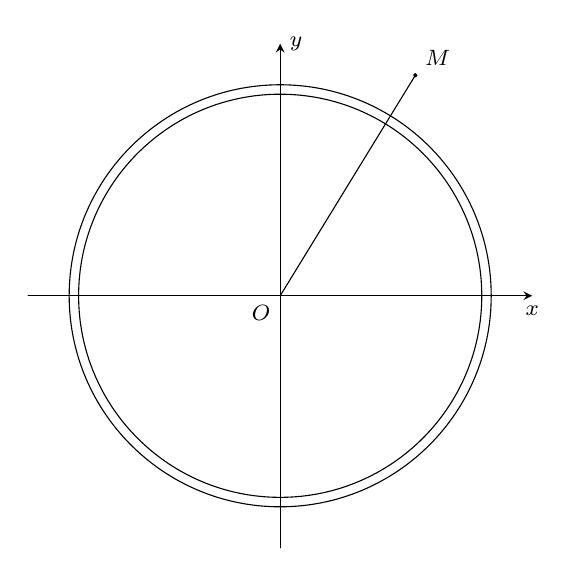
\begin{tikzpicture}[scale=0.4,font=\footnotesize,line join=round,line cap=round,>=stealth]
					\draw[->] (-8,0)--(8,0) node[below]{$x$}; 
					\draw[->] (0,-8)--(0,8) node[right]{$y$}; 
					\draw  (0,0) node[below left] {$O$};
					\draw (0,0) circle (6.4cm); 
					\draw (0,0)  circle (6.7cm);
					\coordinate (A) at (4.29,7); 
					\draw[fill] (A) circle (1.5pt) node[above  right] {$M$};
					\draw  (0,0) -- (A);
				\end{tikzpicture}
		\end{center}
		Ta có $\overrightarrow{OM}=\left(4{,}29;7;0\right)$,  suy ra $OM=\sqrt{4{,}29^2+7^2+0^2}=8{,}21$.\\
		Quảng đường thiên thạch đi từ lúc  phát hiện đến khi bốc cháy là
		\[8{,}21-6{,}4-0{,}15=1{,}66 \, \text{ (ngàn km)}.\] 
		Vậy thời gian thiên thạch bị bốc cháy kể từ lúc  phát hiện là
		 \[\dfrac{1{,}66}{0{,}05}\approx 33 \, \text{ (giây)}.\]
	 }
\end{bt}

% nguồn: Lop_12_Hinh_hoc_Chuong_2
\begin{bt}%[2H2V2-6]%[ma:8a5d9a9a]
	Cho ba lực $\overrightarrow{F}_1=\overrightarrow{MA}$, $\overrightarrow{F}_2=\overrightarrow{MB}$, $\overrightarrow{F}_3=\overrightarrow{MC}$ cùng tác động vào một ô tô tại điểm $M$ và ô tô đứng yên. Cho biết cường độ hai lực $\overrightarrow{F}_1$, $\overrightarrow{F}_2$ đều bằng $25$N và góc $\widehat{AMB}=60^\circ$. Khi đó tính cường độ $\overrightarrow{F}_3$ (làm tròn đến hàng  phần chục).
	\begin{center}
		\begin{tikzpicture}[line join=round,line cap=round,font=\footnotesize,scale=1,>=stealth]
				\def \r{3} 
				 \path
					 (0,0) coordinate (B)
					 (0:\r) coordinate (D)
					(-50:0.5*\r) coordinate (C) 
					($(C)!0.5!(D)$) coordinate (M) 
					($(B)!2/3!(M)$)  coordinate (G_0)
					($(B)!(G_0)!(D)$) coordinate (X) 
					 ($(X)!1.1!90:(D)$) coordinate (A)
					 ($(A)!0.6!(G_0)$) coordinate (G);
				\draw  (A)--(B)--(C)--(D)--(A)--(C);
				 \draw[dashed] (B)--(D)
					 (A)--(G_0)
					(G)--(B)--(M); 
				\foreach \x/\g in {A/90,B/180,C/-90,D/0,M/-30,G_0/-90,G/0}\fill (\x) circle (1pt)+(\g:.3) node{$\x$}; 
			\end{tikzpicture}7
		7 
	\end{center}
	 \shortans{43,3}
	 \loigiai{
		\begin{center}
			\begin{tikzpicture}[line join=round,line cap=round,font=\footnotesize,scale=1,>=stealth]
					\def \r{3} 
					 \path
						(0,0) coordinate  (B)
						(0:\r) coordinate  (D)
						(-50:0.5*\r)  coordinate (C)
						($(C)!0.5!(D)$) coordinate  (M)
						($(B)!2/3!(M)$) coordinate  (G_0)
						($(B)!(G_0)!(D)$) coordinate  (X)
						($(X)!1.1!90:(D)$)  coordinate (A)
						($(A)!0.6!(G_0)$) coordinate (G); 
					 \draw (A)--(B)--(C)--(D)--(A)--(C);
					\draw[dashed]  (B)--(D)
						 (A)--(G_0)
						(G)--(B)--(M); 
					\foreach \x/\g in {A/90,B/180,C/-90,D/0,M/-30,G_0/-90,G/0}\fill (\x) circle (1pt)+(\g:.3) node{$\x$}; 
				\end{tikzpicture}8
			8 
		\end{center}
		Ta có  $\overrightarrow{F_1}+\overrightarrow{F_2}=\overrightarrow{MA}+\overrightarrow{MB}=\overrightarrow{MD}$ (với $D$ là điểm sao cho $AMBD$ là hình bình hành). \\
		 Ta có $MA=\left|\overrightarrow{MA}\right|=\left|\overrightarrow{F}_1\right|=25$N và $MB=\left|\overrightarrow{MB}\right|=\left|\overrightarrow{F}_2\right|=25$N. \\
		Do  $\widehat{AMB}=60^\circ$ nên $\Delta MAB$ là tam giác đều. \\Khi đó $MD=2\cdot \dfrac{25\sqrt{3}}{2}=25\sqrt{3}$ (N).\\
		Do ô tô đứng yên nên cường độ lực tác dụng lên ô tô bằng $0$  hay $\overrightarrow{F}_1+\overrightarrow{F}_2+\overrightarrow{F}_3=\overrightarrow{0}$.\\
		Suy  ra
		$\overrightarrow{F}_3=-(\overrightarrow{F}_1+\overrightarrow{F}_2) 
		\Rightarrow \left|\overrightarrow{F}_3\right|=\left| -(\overrightarrow{F}_1+\overrightarrow{F}_2)\right| 
		=\left|\overrightarrow{DM}\right|=MD=25\sqrt{3}$ (N).\\ 
		Vậy cường độ của $\overrightarrow{F}_3$ là $25\sqrt{3}\approx  43{,}3$ (N).
	 }
\end{bt}

% nguồn: Lop_12_Hinh_hoc_Chuong_2
\begin{bt}%[2H2V2-6]%[ma:6ef71a86]
	\immini{Một kỹ sư thiết kế mô hình trang trí cho một sân khấu nổi có dạng hình lập phương $ABCD\cdot A_1B_1C_1D_1$ với độ dài các cạnh bằng $5~\mathrm{m}$. Để tạo ra nét độc đáo cho sân khấu, người kỹ sư  muốn thiết kế một dàn đèn ánh sáng nối từ một điểm $M$ trên đoạn thẳng $AD_1$ xuống điểm $N$ trên đoạn thẳng $BD$ thỏa mãn $AM=ND$. Dàn đèn ánh sáng có chiều dài ngắn nhất là bao nhiêu mét? (làm tròn kết quả đến hàng phần trăm).
	} 
	{\begin{tikzpicture}
		 \def\a{2}
		\path (0:0) coordinate  (A)
			++(0:\a) coordinate  (D)
			++(-130:\a/2) coordinate (C) 
			($(A)+(C)-(D)$) coordinate (B) 
			($(A)+(90:\a)$) coordinate (A_1) 
			($(B)+(90:\a)$) coordinate  (B_1)
			($(C)+(90:\a)$)  coordinate (C_1)
			($(D)+(90:\a)$) coordinate  (D_1)
			($(A)!1/4!(D_1)$) coordinate  (M)
			($(D)!1/3.7!(B)$) coordinate  (N);
		 \draw[dashed] (B)--(A)--(D)
			 (A)--(A_1)
			(A)--(D_1) 
			 (D)--(B)
			 (M)--(N);
		 \draw (C)--(C_1)
			 (D)--(D_1)
			 (B)--(B_1)
			 (B)--(C)--(D)
			 (A_1)--(B_1)--(C_1)--(D_1)--cycle;
		\foreach \x/\g in {A/180,B/180,C/0,D/0,A_1/180,B_1/180,C_1/0,D_1/0,M/100,N/-130} 
		\fill (\x) circle (1pt) 
			($(\g:4mm)+(\x)$) node  {$\x$};
	\end{tikzpicture}
	 }
	 \shortans{2,89}
	 \loigiai{
		\begin{center}
			\begin{tikzpicture}[line join=round,line cap=round,font=\footnotesize,scale=1,>=stealth]
					 \def \r{3}
					\path 
						(0,0) coordinate  (B)
						 (0:\r) coordinate (D)
						(-40:0.5*\r) coordinate  (C)
						 (60:0.7*\r) coordinate (A)
						($(C)!0.5!(D)$)  coordinate (M)
						($(B)!2/3!(M)$)  coordinate (G);
					\draw (A)--(B)--(C)--(D)--(A)--(C); 
					\draw[dashed]  (B)--(D)
						(A)--(G) 
						 (B)--(M);
					\foreach \x/\g in {A/90,B/180,C/-90,D/0,G/-90,M/-20}\fill (\x)  circle (1pt)+(\g:.3) node{$\x$};
				\end{tikzpicture}8
			8 
		\end{center}
		Chọn hệ trục tọa độ $Oxyz$ có gốc $O$ trùng với điểm $A$, $B$ thuộc tia $Ox$, $D$ thuộc tia $Oy$,  $A_1$ thuộc tia $Oz$.\\
		 Đặt $AM=DN=x\sqrt{2}$ thì $M(0;x;x)$ và $N(x;5-x;0)$.\\
		Do đó $MN^2=6x^2-20x+25=6\left(x-\dfrac{5}{3}\right)^2+\dfrac{25}{3}\ge  \dfrac{25}{3}$.\\
		Vậy $\min  MN=\dfrac{5\sqrt{3}}{3}$.\\
	 }
\end{bt}

% nguồn: Lop_12_Hinh_hoc_Chuong_2
\begin{bt}%[2H2V2-6]%[ma:77774b12]
	Cơn bão Yagi gây thiệt hại nghiêm trọng về người và tài sản cho nước ta,  trong đó nặng nề nhất là tại thôn Làng Nủ, xã Phúc Khánh, huyện Bảo Yên, tỉnh Lào Cai, lũ quét và sạt lở đất đã vùi lấp 40 ngôi nhà. Cả nước đã chung tay ủng hộ và xây dựng lại nhà sàn cho người dân Làng Nủ theo thiết kế như hình vẽ dưới đây.
	\begin{center}
		\begin{tikzpicture}[line join = round,line cap = round,>=stealth,font=\footnotesize,scale=1]
				 \path
					(0,0) coordinate (O) 
					(0,4) coordinate (I) node[above  left]{$8$}
					 (2.25,4) coordinate (C)
					 (-2.3,4) coordinate (E)
					(2.34,-1.68) coordinate  (H)
					(-5,-1.68) coordinate  (K)
					(-5,1.64) coordinate (G) 
					(2.38,1.64)  coordinate (A)
					(4,0) coordinate (M)  node[below]{$6$}
					(4,3)  coordinate (B)
					(1.38,2.66) coordinate  (D)
					 (-3.3,2.66) coordinate (F)
					(2.82,3.44)  coordinate (R)
					(-1.6,-1.68) node[below]{$6$}; 
				\draw[->,dashed] (O)  -- (-3,-3) node[left] {$x$};
				 \draw[->,dashed] (O) -- (5,0) node[above] {$y$};
				\draw[->,dashed]  (O) -- (0,5) node[right] {$z$};
				 \draw (E) -- (C)
					 (H)--(K)--(G)--(A)--(H)
					(A)--(B)--(M)--(H) 
					(A)--(D)--(C)--(R)--(B) 
					 (G)--(F)--(E);
				\foreach \x/\g in  {O/180,I/60,C/90,E/90,G/180,A/90,B/70,D/180,F/90} \fill (\x) circle (1pt)+(\g:3mm) node{$\x$};
			\end{tikzpicture}
	\end{center}
	Giả sử áp dụng hệ trục tọa độ $Oxyz$ như hình vẽ (đơn vị trên các trục là mét). Xét một bên của mái nhà gồm có một hình chữ nhật $CDFE$ và một hình thang $ADFG$ với các điểm $G(6;-6;6)$; $C(3;4;8)$; $F(4;-4;7)$ và điểm $I$ là trung  điểm $CE$. Biết góc giữa hai vectơ $\overrightarrow{DC}$ và $\overrightarrow{AB}$ bằng $a^\circ$. Tìm $a$ (kết quả làm tròn đến hàng đơn vị).
	 \shortans{45}
	 \loigiai{
		Xét hệ  trục tọa độ $Oxyz$, ta có:\\
		$A$, $G$ đối xứng qua  $(Oxz)$ nên tọa độ điểm $A$ là $A(6;6;6)$.\\
		$AB\parallel (Oxy)$ và  $B\in (Oyz)$ nên tọa độ điểm $B$ là $B(0;6;6)$.\\
		$D$, $F$ đối  xứng qua $(Oxz)$ nên tọa độ điểm $D$ là $D(4;4;7)$.\\
		 Khi đó $\overrightarrow{AB}=(-6;0;0)$; $\overrightarrow{DC}=(-1;0;1)$.\\
		 $$\cos\alpha=\cos\left(\overrightarrow{DC},\overrightarrow{AB}\right)=
		\dfrac{\overrightarrow{DC}\cdot \overrightarrow{AB}}{|\overrightarrow{DC}|\cdot |\overrightarrow{AB}|}=\dfrac{(-6)\cdot (-1)+0\cdot 0+0\cdot 1}{\sqrt{(-6)^2+0^2+0^2}\cdot \sqrt{(-1)^2+0^2+1^2}}=\dfrac{\sqrt{2}}{2}.$$ 
		Vậy  $\alpha =45^\circ$.
	} 
\end{bt}

% nguồn: Lop_12_Hinh_hoc_Chuong_2
\begin{bt}%[2H2V2-6]%[ma:b989a396]
	Ba chiếc máy bay không người lái cùng bay lên tại một địa điểm. Sau một thời gian bay, chiếc máy bay thứ nhất cách điểm xuất phát về phía Đông $60$ km và về phía Nam $40$ km, đồng  thời cách mặt đất $2$ km. Chiếc máy bay thứ hai cách điểm xuất phát về phía Bắc $80$ km và về phía Tây $50$ km, đồng thời cách mặt đất $4$ km. Chiếc máy bay thứ ba nằm chính giữa của chiếc máy bay thứ nhất và thứ hai, đồng thời ba chiếc máy bay này thẳng hàng. Xác định khoảng cách của chiếc máy bay thứ ba với vị trí tại điểm xuất phát của nó. (\textit{Kết quả làm tròn đến hàng phần chục})
	 \shortans{11,6}
	\loigiai{Chọn  hệ trục tọa độ $Oxyz$, với gốc đặt tại điểm xuất phát của hai chiếc máy bay, mặt phẳng $(Oxy)$ trùng với mặt đất, trục $Ox$ hướng về phía Bắc, trục $Oy$ hướng về phía Tây, trục $Oz$ hướng thẳng đứng lên trời, đơn vị đo lấy theo kilômét (xem hình vẽ).
		\begin{center}
			\begin{tikzpicture}[line join=round,line cap=round,>=stealth,scale=0.6,font=\footnotesize]
					\foreach \x/\y/\n in  {0/0/A,6/0/C,2/-2/B} \coordinate (\n) at (\x,\y);
					 \coordinate (S) at ($(A)+(0,4)$);
					\coordinate (M) at ($(B)!1/2!(C)$); 
					\coordinate (G) at ($(A)!2/3!(M)$); 
					 \draw (S)--(A)--(B)--(C)--(S)--(B);
					\draw[dashed] (A)--(C) 
						 (A)--(M);
					\foreach \t/\g in  {A/180,B/-110,C/0,S/90,M/-40,G/-90}{
						\fill (\t)  circle (1pt) node[shift={(\g:8pt)}]{$ \t $};
					} 
					\draw pic[thin,draw,angle radius=2mm] {right  angle= A--B--C};
				\end{tikzpicture}3
			 3
		\end{center}
		Chiếc  máy bay thứ nhất có tọa độ $(-60;-40;2)$.\\
		Chiếc máy bay thứ hai có tọa  độ $(80;50;4)$.\\
		Do chiếc máy bay thứ ba nằm chính giữa của chiếc máy bay thứ nhất và thứ hai, đồng thời ba chiếc máy bay này thẳng hàng nên ở vị trí trung điểm, suy ra chiếc máy bay thứ ba có tọa độ  $$\left(\dfrac{-60+80}{2};\dfrac{-40+50}{2};\dfrac{2+4}{2}\right)=(10;5;3).$$
		 Khoảng cách của chiếc máy bay thứ ba với vị trí tại điểm xuất phát của nó là
		$$ 
		\sqrt{10^2+5^2+3^2}  \approx 11{,}6(\mathrm{~km}).
		$$ 
	} 
\end{bt}

% nguồn: Lop_12_Hinh_hoc_Chuong_2
\begin{bt}%[2H2V2-6]%[ma:dba494bc]
	Có ba lực cùng tác động vào một  vật. Hai trong ba lực này hợp với nhau một góc $100^\circ$ và có độ lớn lần lượt là $25$ N và $12$ N. Lực thứ ba vuông góc với mặt phẳng tạo bởi hai lực đã cho và có độ lớn $4$ N. Tính độ lớn của hợp lực (N) của ba lực trên (làm tròn kết quả đến hàng đơn vị).
	\begin{center}
		\begin{tikzpicture}[scale=0.7,font=\footnotesize,line join=round,line cap=round]
				\foreach \x\y\t  in {0/0/O,-2/-1.3/B,4/0/A,0/3/C}
				\coordinate (\t) at  (\x,\y);
				\coordinate (D) at  ($(A)+(B)$);
				\coordinate  (E) at ($(C)+(D)$);
				\coordinate (x) at (intersection of A--O  and E--D);
				\path (x)--(A)  node[pos=0.5,above]{$\overrightarrow{F_1}$};
				 \path (O)--(B) node[pos=0.5,above left]{$\overrightarrow{F_2}$};
				\path (O)--(C) node[pos=0.5,left]{$\overrightarrow{F_3}$}; 
				\path (O)  pic[draw,angle radius=6]{angle=B--O--A}node[shift={(-85:10pt)}]{$100^{\circ}$};
				\foreach \a\b in  {O/B,x/A,O/D,O/C,O/E}
				 \draw[-{Stealth[length=2mm]}] (\a)--(\b);
				\draw  (B)--(D)--(A)
					(C)--(E)--(D); 
				\draw[dashed]  (O)--(x);
				\foreach \t\g  in {O/170,A/90,B/150,C/90,D/-80,E/45}
				\draw (\t) circle (0.6pt)  +(\g:8pt) node{$\t$};
			\end{tikzpicture}
	\end{center}
	 \shortans{26}
	 \loigiai{
		Hợp lực của hai lực đầu tiên là $\overrightarrow{F}_{12}=\overrightarrow{F}_{1}+\overrightarrow{F}_{2}$.\\ 
		Độ lớn hợp lực của hai lực đó là  $\left|\overrightarrow{F}_{12}\right|=\sqrt{{F}_{1}^{2}+{F}_{2}^{2}+2 \cdot F_1 \cdot F_2 \cdot \cos \left(F_1, F_2\right)}=25{,}78$ (N).\\
		Lực $\overrightarrow{F}_{3}$ vuông góc với mặt phẳng tạo bởi hai lực đã cho nên $\overrightarrow{F}_{3}$ vuông góc với mọi véc-tơ nằm trong mặt phẳng tạo bởi $\overrightarrow{F}_{1}$ và $\overrightarrow{F}_{2}$. 
		 \[\left|\overrightarrow{F}\right|=\left|\overrightarrow{F}_{3}+\overrightarrow{F}_{12}\right|=\sqrt{F_{3}^{2}+F_{12}^{2}+2 \cdot F_3 \cdot F_{12} \cdot \cos \left(F_3, F_{12}\right)}=26\,(\mathrm{N}).\]
		Vậy độ lớn tổng hợp lực là $26$ (N). 
	} 
\end{bt}

% nguồn: Lop_12_Hinh_hoc_Chuong_2
\begin{bt}%[2H2V2-6]%[ma:5af671fd]
	Trong hệ trục $Oxyz$ cho trước (đơn vị trên trục là mét), cho một trạm thu phát sóng 5G có bán kính vùng phủ sóng của trạm ở ngưỡng 600 m được đặt ở vị trí $I(200; 450; 60)$. Tìm giá trị lớn nhất cúa $m$ (làm tròn đên hàng đơn vị) để một  người dùng điện thoại ở vị trí $A(m+100; m+370; 0)$ có thể sử dụng dịch vụ của trạm nói trên.
	\shortans{512} 
	 \loigiai{
		Để một người dùng điện thoại ở vị trí $A(m+100; m+370; 0)$ có thể sử dụng dịch vụ của trạm thu phát sóng 5G có bán kính vìng phủ sóng của trạm ở ngưỡng 600 m được đặt ở vị trí $I(200; 450;  60)$ thì
		\begin{align*}
			I A \leq  600 &\Leftrightarrow(m-100)^2+(m-80)^2+(-60)^2 \leq 600^2\\
			&\Leftrightarrow 2 m^2-360 m-340000 \leq 0\\ &\Leftrightarrow 90-10 \sqrt{1781} \leq m  \leq 90+10 \sqrt{1781}.
		\end{align*}
		Vậy giá trị lớn nhất của $m$ là $90+10 \sqrt{1781} \approx 512$. 
	 }
\end{bt}

% nguồn: Lop_12_Hinh_hoc_Chuong_2
\begin{bt}%[2H2V2-6]%[ma:dd227759]
	Hai chiếc khinh khí cầu bay lên từ cùng một địa điểm. Sau một thời gian chiếc thứ nhất cách điểm xuất phát $300$ m về phía Nam và $100$ m về phía Đông, đồng thời cách mặt đất $100$ m. Chiếc thứ hai nằm  cách điểm xuất phát $200$ m về phía Bắc và $100$ m về phía Tây, đồng thời cách mặt đất $50$ m. Cùng thời điểm đó, một người đứng trên mặt đất quan sát thấy hai chiếc khinh khí cầu nói trên. Biết rằng, so với các vị trí quan sát trên mặt đất, vị trí người đứng có tổng khoảng cách đến hai chiếc khinh khí cầu là nhỏ nhất. Tính khoảng cách từ vị trí người quan sát đến địa điểm xuất phát của hai chiếc khinh khí cầu (kết quả làm tròn đến hàng đơn vị).
	 \shortans{47}
	\loigiai{ 
		Chọn hệ trục $Oxyz$ với gốc $O$ đặt tại điểm xuất phát của hai khinh khí cầu, mặt phẳng $(Oxy)$ trùng với mặt đất với trục $Ox$ hướng về phía Nam, trục $Oy$ hướng về phía Đông và trục $Oz$ hướng thẳng đứng lên trời, đơn vị đo lấy theo mét.  \\
		Gọi $A$, $B$, $M$ lần lượt là vị trí của khinh khí cầu thứ nhất, khinh khí  cầu thứ hai và người quan sát.
		\begin{center}
			\begin{tikzpicture}[smooth,samples=300,scale=0.8,>=stealth,font=\footnotesize]
					\draw[->] (-4,0) node[above right]{Bắc}--(6,0) node[below]{$x$} node[above  left]{Nam};
					\draw[->] (3,3) node[above right]{Tây}--(-2.3,-2.3)  node[left]{$y$}node[below right]{Đông};
					\draw[->] (0,0)--(0,4.5) node[right]{$z$}; 
					\draw (0,0) node[below]{$O$}; 
					\fill [scale=.1,yshift=12  cm,xshift=25 cm]
						(-1,0)  rectangle (1,1)
						(-1,2).. controls +(135:1) and +(180:4)..  (0,7)
						..  controls +(180:2) and +(135:2).. (-.5,2)
						.. controls +(120:2)  and +(180:1).. (0,6.99)
						.. controls +(0:1) and  +(60:2).. (.5,2)
						 .. controls +(45:2) and +(0:2).. (0,7)
						.. controls  +(0:4) and +(45:1).. (1,2);
					 \draw[scale=.1,yshift=12 cm,xshift=25 cm] (-1,0) rectangle (1,2)
						 (0,1)--(0,2);;
					 \fill [scale=.1,blue,yshift=37 cm,xshift=-20 cm]
						(-1,0)  rectangle (1,1)
						 (-1,2).. controls +(135:1) and +(180:4).. (0,7)
						.. controls +(180:2)  and +(135:2).. (-.5,2)
						..  controls +(120:2) and +(180:1).. (0,6.99)
						.. controls +(0:1) and  +(60:2).. (.5,2)
						 .. controls +(45:2) and +(0:2).. (0,7)
						.. controls +(0:4) and +(45:1).. (1,2); 
					\draw[blue,scale=.1,yshift=37 cm,xshift=-20 cm] (-1,0) rectangle  (1,2)
						(0,1)--(0,2);; 
					 \draw[dashed] (4,0)--(2.5,-1.5)--(-1.5,-1.5)
						(2.5,1)--(0,0)--(2.5,-1.5)--(2.5,1); 
					\draw[dashed] (-3,0)--(-2,1)--(1,1) 
						(-2,1)--(0,0)--(-2,3.5)--(-2,1); 
					\draw  (2.5,1) circle (2pt)
						(-2,3.5) circle (2pt); 
				\end{tikzpicture}
		\end{center}
		Khi đó $A(300;100;100)$, $B(-200;-100;50)$,  $M(a;b;0)$.\\
		Gọi $B'$ là điểm đối  xứng của $B$ qua mặt phẳng $(Oxy)$.\\
		 Suy ra $B'(-200;-100;-50)$.\\
		Ta có $MA +  MB = MA + MB' \geq AB'$.\\
		 Do đó $MA + MB$ nhỏ nhất khi bằng $AB'$, hay $M$ là giao điểm của $AB'$ với mặt phẳng $(Oxy)$. \\
		Suy ra $A$, $B'$, $M$ thẳng  hàng hay $\overrightarrow{AM}$, $\overrightarrow{AB'}$ cùng phương. \\
		Có  $\overrightarrow{AM} = (a-300; b-100;-100)$, $\overrightarrow{AB'}=(-500;-200;-150)$.\\
		 Suy ra
		$$\dfrac{a-300}{-500} = \dfrac{b-100}{-200} = \dfrac{-100}{-150} = \dfrac{2}{3}\Rightarrow  \heva{&a = -\dfrac{100}{3} \\& b = -\dfrac{100}{3}}.$$
		Suy ra $M\left(-\dfrac{100}{3}; -\dfrac{100}{3}; 0\right).$  \\
		Vậy khoảng cách từ vị trí  người quan sát đến địa điểm xuất phát của hai chiếc khinh khí cầu là $OM = \dfrac{100\sqrt{2}}{3} \approx 47$.
	 }
\end{bt}

% nguồn: Lop_12_Hinh_hoc_Chuong_2
\begin{bt}%[2H2V2-6]%[ma:b9fae808]
	Trong không gian với hệ trục tọa độ $Oxyz$, một cabin cáp treo xuất phát từ phía  $A (10; 3; 0)$ và chuyển động theo đường cáp có vectơ chỉ phương là $\vec{u}=(2; -2; 1)$ với tốc độ $4{,}5$ m/s (đơn vị trên mỗi trục tọa độ là mét). Một camera giám sát an toàn đặt tại $I(50; -10; 50)$. Hỏi sau bao nhiêu giây kể từ khi cabin xuất phát thì cabin gần camera an toàn nhất? (kết quả làm tròn đến hàng đơn vị)
	\shortans{12} 
	\loigiai{ 
		Độ  lớn của vectơ $\vec{u}$ là $\left|\vec{u}\right|=\sqrt{2^2+(-2)^2+1^2}=3$.\\
		Vectơ  vận tốc $\vec{v}$ là \[\vec{v}=\dfrac{4{,}5}{\left|\vec{u}\right|}\vec{u}=\dfrac{4{,}5}{3}(2; -2; 1)=(3; -3; 1{,}5).\]
		Khi đó, ta có thể biểu diễn tọa độ cabintại thời điểm $t (\mathrm{s})$ như  sau $M(10+3t; 3-3t; 1{,}5t)$.\\
		Do camera đặt tại điểm $I(50; -10; 50)$ nên  khoảng cách từ camera đến cabin là \[MI=\sqrt{(10+3t-50)^2+(3-3t+10)^2+(1{,}5t-50)^2}=\sqrt{(3t-40)^2+(13-3t)^2+(1{,}5t-50)^2}.\]
		 Xét hàm $f(t)=MI^2=(3t-40)^2+(13-3t)^2+(1{,}5t-50)^2$.\\
		 Ta có $f(t)=20{,}25t^2-468t+4269$.\\
		Suy ra $f'(t)=40{,}5t-468=0\Leftrightarrow t=\dfrac{104}{9}\approx 12$.\\ 
		Do  đó $\min\limits_{[0;+\infty)}f(t)=f\left(12\right)$.
	} 
\end{bt}

% nguồn: Lop_12_Hinh_hoc_Chuong_2
\begin{bt}%[2H2V2-6]%[ma:77c8967f]
	Trong không gian  với hệ trục tọa độ $Oxyz$ (đơn vị trên mỗi trục là mét), một thiết bị phát sóng wifi được đặt tại vị trí $I(3; 4; 2)$. Vùng phủ sóng của thiết bị là một hình cầu có bán kính $R=10$ m. Một người sử dụng điện thoại ở vị trí $K (x-7; 7; 1)$. Sau đó người đó di chuyển đến vị trí $H (x+11; 7; 1)$. Tìm giá trị $x$ nguyên sao cho cả hai vị trí $K$ và $H$ đều có thể bắt được tín hiệu wifi từ thiết bị.
	\shortans{1} 
	 \loigiai{
	Tại vị trí $H$ và $K$ có thể bắt được  sóng wifi khi và chỉ khi hệ sau được thỏa mãn
	\begin{align*}
		\heva{&IK \le 10\\&IH\le 10}\Leftrightarrow&\heva{&(x-10)^2+(7-4)^2+(1-2)^2\le 100\\&(x+8)^2+(7-4)^2+(1-2)^2\le 100}\\ 
		\Leftrightarrow&\heva{&(x-10)^2\le90\\&(x+8)^2\le 90}\\ 
		\Leftrightarrow&\heva{&10-\sqrt{90}\le x\le 10+\sqrt{90}\\&-8-\sqrt{90}\le x\le  -8+\sqrt{90}}\\
		\Leftrightarrow& 10-\sqrt{90}\le x\le -8+\sqrt{90}\,\,\, (*). 
	\end{align*}
	Mà  $x\in\mathbb{Z}$ nên suy ra $x=1$.\\
	 Vậy $x=1$.
	 }
\end{bt}

% nguồn: Lop_12_Hinh_hoc_Chuong_2
\begin{bt}%[2H2V2-6]%[ma:f536bb32]
	Hai  chiếc khinh khí cầu cùng bay lên tại một địa điểm. Sau một thời gian bay, chiếc khinh khí cầu thứ nhất cách điểm xuất phát về phía Đông $100$ km và về phía Nam $80$ km, đồng thời cách mặt đất $1$ km. Chiếc khinh khí cầu thứ hai cách điểm xuất phát về phía Bắc $70$ km và về phía Tây $60$ km, đồng thời cách mặt đất $0,8$ km.
	Xác định khoảng cách giữa chiếc khinh khí cầu thứ nhất và chiếc khinh khí cầu thứ hai. (\textit{Kết quả làm tròn đến hàng đơn  vị})
	 \shortans{220}
	\loigiai{Chọn hệ trục tọa độ $Oxyz$, với gốc đặt tại điểm xuất phát của hai chiếc khinh khí cầu, mặt phẳng $(Oxy)$  trùng với mặt đất, trục $Ox$ hướng về phía Bắc, trục $Oy$ hướng về phía Tây, trục $Oz$ hướng thẳng đứng lên trời, đơn vị đo lấy theo kilômét (xem hình vẽ).
		\begin{center}
			\begin{tikzpicture}[line join=round,line cap=round,>=stealth,scale=0.6,font=\footnotesize]
					\foreach \x/\y/\n in {0/0/A,6/0/C,2/-2/B} \coordinate (\n) at (\x,\y); 
					\coordinate (S)  at ($(A)+(0,4)$);
					\coordinate  (M) at ($(B)!1/2!(C)$);
					\coordinate (G) at ($(A)!2/3!(M)$); 
					\draw (S)--(A)--(B)--(C)--(S)--(B); 
					\draw[dashed]  (A)--(C)
						(A)--(M); 
					\foreach \t/\g in  {A/180,B/-110,C/0,S/90,M/-40,G/-90}{
						\fill (\t) circle  (1pt) node[shift={(\g:8pt)}]{$ \t $};
					} 
					\draw pic[thin,draw,angle radius=2mm] {right angle=  A--B--C};
				\end{tikzpicture}1
			 1
		\end{center}
		Chiếc khinh khí  cầu thứ nhất có tọa độ $(-100;-80;1)$.\\
		Chiếc khinh khí cầu thứ hai  có tọa độ $(70;60;0,8)$.\\
		Khoảng cách giữa  chiếc khinh khí cầu thứ nhất và chiếc khinh khí cầu thứ hai là
		$$\sqrt{(-100-70)^2+(-80-60)^2+(1-0,8)^2} \approx  220~(\text{km}).$$
	} 
\end{bt}

% nguồn: Lop_12_Hinh_hoc_Chuong_2
\begin{bt}%[2H2V2-6]%[ma:c9551a08]
	Một chiếc máy bay đang bay trong không gian $Oxyz$, với tọa độ hiện tại là $M\left(40;10;40\right)$. Đường bay mong muốn của  máy bay đi qua hai điểm $A\left(0;10;0\right)$ và $B\left(20;0;10\right)$. Hãy tìm khoảng cách ngắn nhất từ vị trí hiện tại của máy bay đến đường bay mong muốn này. Kết quả làm tròn đến hàng phần mười.\\
	\shortans{28,3} 
	\loigiai{ 
		Gọi $H\left(x;y;z\right)$ là hình chiếu của $M$ trên đường thẳng $AB$. Khi đó $\min  \mathrm{d}\left(M;AB\right)=MH$.\\
		Có $\overrightarrow{MH}=\left(x-40;y-10;z-40\right)$, $\overrightarrow{AH}=\left(x;y-10;z\right)$, $\overrightarrow{AB}=\left(20;-10;10\right)$.\\ 
		Vì $MH\perp  AB$ và vectơ $\overrightarrow{AH}$, $\overrightarrow{AB}$ cùng phương nên
		\begin{eqnarray*}
			 &&\heva{&20\left(x-40\right)-10\left(y-10\right)+10\left(z-40\right)=0 \\&\dfrac{x}{20}=\dfrac{y-10}{-10}=\dfrac{z}{10}}\\
			&\Rightarrow  &\heva{&2x-y+z-110=0 \\&x=2z \\&y=10-z}\\
			&\Rightarrow  &\heva{&x=40 \\&y=-10 \\&z=20.}
		\end{eqnarray*}
		 Suy ra $H\left(40;-10;20\right)$.\\
	Do đó $MH=20\sqrt{2}\approx  28{,}3$.}
\end{bt}

% nguồn: Lop_12_Hinh_hoc_Chuong_2
\begin{bt}%[2H2V2-6]%[ma:b174b040]
	Hệ thống định vị toàn cầu GPS (Global Positioning System) là một hệ thống cho phép xác định vị trí của một vật thể trong không gian. Trong cùng một thời điểm, vị trí của một điểm $M$ trong không gian sẽ đươc  xác định bởi bốn vệ tinh cho trước nhờ các bộ thu phát tín hiệu đặt trên các vệ tinh. Giả sử trong không gian với hệ trục tọa độ $Oxyz$, có bốn vệ tinh đặt tại các điểm có tọa độ lần lượt là $A(0;4;5)$, $B(-3;-1;3)$, $C(-2;8;9)$, $D(-7;2;-3)$ đang tiến hành theo dõi vật thể $M$ (coi là một chất điểm). Tại một thời điểm, cả bốn vệ tinh đồng thời phát tín hiệu về điểm $M$ và ngay lập tức nhận lại tín hiệu phản hồi sau những khoảng thời gian lần lượt là $t_A=0{,}2\ \mathrm{ms}$, $t_B=\dfrac{1}{3}\ \mathrm{ms}$, $t_C=0{,}6\ \mathrm{ms}$, $t_D=\dfrac{2}{3} ms$. Biết rằng vận tốc của sóng điện từ bằng vận tốc ánh sáng $c=3\cdot10^8\ \mathrm{m/s}$. Tính khoảng cách từ $M$ đến $O$ biết một đơn vị độ dài trên các trục bằng $10\ \mathrm{km}$ thực tế (đơn vị: $\mathrm{km}$, kết quả làm tròn đến hàng phần chục).
	\begin{center}
		\begin{tikzpicture}[line join=round,line cap=round,font=\footnotesize,scale=1,>=stealth]
				 \def \r{3}
				 \path
					(0,0) coordinate  (B)
					(0:\r)  coordinate (D)
					(-40:0.5*\r) coordinate (C) 
					(60:0.7*\r) coordinate (A) 
					($(C)!0.5!(D)$) coordinate (M) 
					($(B)!2/3!(M)$) coordinate  (G);
				\draw  (A)--(B)--(C)--(D)--(A)--(C);
				 \draw[dashed] (B)--(D)
					(A)--(G) 
					(B)--(M); 
				\foreach \x/\g in {A/90,B/180,C/-90,D/0,G/-90,M/-20}\fill  (\x) circle (1pt)+(\g:.3) node{$\x$};
			\end{tikzpicture}4
		 4
	\end{center}
	 \shortans{37,4}
	 \loigiai{
		Gọi  $M(x;y;z)$.\\
		Do mỗi vệ tinh  gửi tín hiệu đến $M$ và nhận lại phản hồi sau thời gian $t$, tức tín hiệu đi từ vệ tinh đến $M$ và quay về nên quãng đường đi được là gấp đôi nên\\
		$MA=\dfrac{0{,}2\cdot  10^{-3}\cdot3\cdot10^8}{2}=30\ 000\ \mathrm{m}=30\ \mathrm{km}$;\\
		$MB=\dfrac{\dfrac{1}{3}\cdot10^{-3}\cdot3\cdot10^8}{2}=50\ 000\ \mathrm{m}=50\ \mathrm{km}$;\\ 
		 $MC=\dfrac{0{,}6\cdot10^{-3}\cdot3\cdot10^8}{2}=90\ 000\ \mathrm{m}=90\ \mathrm{km}$;\\
		$MD=\dfrac{\dfrac{2}{3}\cdot10^{-3}\cdot3\cdot10^8}{2}=100\  000\ \mathrm{m}=100\ \mathrm{km}$.\\
		Do mỗi đơn vị độ dài  trên các trục bằng $10\ \mathrm{km}$ nên\\ $\heva{&x^2+(y-4)^2+(z-5)^2=3^2\\&(x+3)^2+(y+1)^2+(z-3)^2=5^2\\&(x+2)^2+(y-8)^2+(z-9)^2=9^2\\&(x+7)^2+(y-2)^2+(z+3)^2=10^2}\Leftrightarrow\heva{&x^2+y^2+z^2-8y-10z=-32\\&x^2+y^2+z^2+6x+2y-6z=6\\&x^2+y^2+z^2+4x-16y-18z=-68\\&x^2+y^2+z^2+14x-4y+6z=38}$\\
		$\Leftrightarrow\heva{&-6x-10y-4z=-38\\&-4x+8y+8z=36\\&-14x-4y-16z=-70}\Leftrightarrow\heva{&x=1\\&y=2\\&z=3}$.\\ 
		Suy ra $OM=\sqrt{1^2+2^2+3^2}=\sqrt{14}$.\\ 
		Vậy khoảng cách  từ $O$ đến $M$ là $\sqrt{14}\cdot10\approx37{,}4\mathrm{km}$.
	} 
\end{bt}

% nguồn: Lop_12_Hinh_hoc_Chuong_2
\begin{bt}%[2H2V2-6]%[ma:4fa7f355]
	\immini[thm]{Một công ty logistics đang thử nghiệm hệ thống giao hàng tự động bằng máy bay không người lái (drone). Trong không gian $Oxyz$, mỗi đơn vị trên các trục tương ứng với $1$ mét trên thực tế. Mặt ngoài của một tòa nhà cao tầng được xem là một phần của  mặt phẳng $(P)$ thẳng đứng, đi qua hai điểm $C(10;50;0)$ và $D(30;10;0)$.
	 }{
	\begin{tikzpicture}[line join=round,line cap=round,font=\footnotesize,scale=1,>=stealth]
			\def \r{3} 
			 \path
				(0,0) coordinate (B) 
				(0:\r) coordinate (D) 
				(-50:0.5*\r) coordinate  (C)
				($(C)!0.5!(D)$)  coordinate (M)
				($(B)!2/3!(M)$) coordinate  (G_0)
				($(B)!(G_0)!(D)$) coordinate (X) 
				($(X)!1.1!90:(D)$) coordinate (A) 
				($(A)!0.6!(G_0)$) coordinate (G); 
			\draw (A)--(B)--(C)--(D)--(A)--(C); 
			 \draw[dashed] (B)--(D)
				 (A)--(G_0)
				 (G)--(B)--(M);
			\foreach \x/\g  in {A/90,B/180,C/-90,D/0,M/-30,G_0/-90,G/0}\fill (\x) circle (1pt)+(\g:.3) node{$\x$};
		\end{tikzpicture}9
	 9
	 }\noindent
	Vị trí giao hàng là điểm $B$ nằm trên mặt phẳng $(P)$.  Drone bắt đầu bay từ kho hàng tại gốc tọa độ $O(0;0;0)$. Ban đầu, nó bay theo một đường thẳng đến vị trí $A(30;40;120)$. Từ vị trí $A$, drone thay đổi đường bay, di chuyển theo phương vuông góc với mặt phẳng $(P)$ đến vị trí giao hàng $B$. Tính khoảng cách từ $O$ đến $B$ (làm tròn đến hàng đơn vị).
	 \shortans{126}
	 \loigiai{
		Ta  có $\overrightarrow{CD}=(20;-40;0)=20\overrightarrow{u}$ với $\overrightarrow{u}=(1;-2;0)$.\\
		Do $(P)$ là mặt phẳng thẳng đứng qua $C$ và $D$ nên nhận vec-tơ $\overrightarrow{u}=(1;-2;0)$ và $\overrightarrow{k}=(0;0;1)$ làm cặp vec-tơ  chỉ phương nên vec-tơ pháp tuyến của $(P)$ là $\overrightarrow{n}=\left[\overrightarrow{u},\overrightarrow{k}\right]=(-2;-1;0)$ hay $\overrightarrow{n}=(2;1;0)$.\\
		Phương trình mặt phẳng $(P) \colon 2(x-10)+1(y-50)+0(z-0)=0 \Leftrightarrow  2x+y-70=0$.\\
		Đường thẳng $AB$ vuông góc với $(P)$ nên nhận vec-tơ pháp tuyến của  $(P)$ làm vec-tơ chỉ phương $\overrightarrow{u}_{AB}=(2;1;0)$ nên có phương trình đường thẳng $AB \colon$ $\heva{&x=30+2t\\&y=40+t\\&z=120.}$\\
		Vì $B$ là giao điểm của  đường thẳng $AB$ và mặt phẳng $(P)$ nên ta có
		\allowdisplaybreaks 
		\begin{eqnarray*}
			 &&2(30+2t)+(40+t)-70=0\\
			 &\Leftrightarrow&5t+30=0 \\
			&\Leftrightarrow&5t=-30  \\
			&\Leftrightarrow&t=-6. 
		\end{eqnarray*}
		Từ đó suy  ra $B(18;34;120) \Rightarrow OB=\sqrt{18^2+34^2+120^2}=126$.
	 }
\end{bt}

% nguồn: Lop_12_Hinh_hoc_Chuong_2
\begin{bt}%[2H2V2-6]%[ma:f65f6286]
	Có ba lực $F_1$, $F_2$, $F_3$ cùng tác động vào một vật. Ba lực này đôi một hợp với nhau một góc $60^\circ$ và có độ lớn lần lượt là $3$ N, $6$ N và $9$ N. Tính độ lớn (N) của hợp lực của ba lực trên. 
	\shortans{15} 
	 \loigiai{
		Đặt $\overrightarrow{F}_{1}=\overrightarrow{a}$; $\overrightarrow{F}_{2}=\overrightarrow{b}$;  $\overrightarrow{F}_{3}=\overrightarrow{c}$ ta được $\left|\overrightarrow{a}\right|=3$, $\left|\overrightarrow{b}\right|=6$, $\left|\overrightarrow{c}\right|=9$.\\
		Vì ba lực này đôi một hợp với nhau một góc $60^\circ$  nên $\left(\overrightarrow{a}; \overrightarrow{b}\right)=\left(\overrightarrow{b}; \overrightarrow{c}\right)=\left(\overrightarrow{c}; \overrightarrow{a}\right)=60^{\circ}$\\
		Ta có  $\overrightarrow{F}=\overrightarrow{a}+\overrightarrow{b}+\overrightarrow{c}$, nên
		\begin{eqnarray*}
			\left|\overrightarrow{F}\right|^{2}&=&\left(\overrightarrow{a}+\overrightarrow{b}+\overrightarrow{c}\right)^{2}  \\&=&
			 \left|\overrightarrow{a}\right|^{2}+\left|\overrightarrow{b}\right|^{2}+\left|\overrightarrow{c}\right|^{2}+2 \overrightarrow{a} \cdot \overrightarrow{b}+2 \overrightarrow{a} \cdot \overrightarrow{c}+2 \overrightarrow{b} \cdot \overrightarrow{c} \\
			 &=&9+36+81+18+54+27=225.
		\end{eqnarray*}
		 Vậy $\left|\overrightarrow{F}\right|=15$ (N).
	} 
\end{bt}

% nguồn: Lop_12_Hinh_hoc_Chuong_2
\begin{bt}%[2H2V2-6]%[ma:115a5ad5]
	\immini[thm]{Hai chiếc flycam được điều khiển cùng bay lên tại một địa điểm. Sau một thời gian bay, chiếc flycam thứ nhất bay đến vị trí điểm $A$ cách mặt đất $5$ m, cách điểm xuất phát $3$ m về phía nam và $2$ m về phía đông. Chiếc flycam thứ hai bay đến điểm $B$ cách mặt đất $5$ m, cách điểm xuất phát $6$ m về phía bắc và $6$ m về phía Tây. Chọn hệ trục tọa độ $Oxyz$ với gốc $O$ đặt tại điểm xuất  phát của hai chiếc flycam, mặt phẳng $(Oxy)$ trùng với mặt đất (coi như phẳng) có trục $Ox$ hướng về phía nam, trục $Oy$ hướng về phía đông và trục $Oz$ hướng thẳng đứng lên trời (đơn vị đo mỗi trục là mét).}
	 {
	\begin{tikzpicture}[line join=round,line cap=round,font=\footnotesize,scale=1,>=stealth]
			\def  \r{3}
			\path 
				(0,0) coordinate (B) 
				 (0:\r) coordinate (D)
				(-50:0.5*\r) coordinate (C) 
				 ($(C)!0.5!(D)$) coordinate (M)
				($(B)!2/3!(M)$)  coordinate (G_0)
				 ($(B)!(G_0)!(D)$) coordinate (X)
				($(X)!1.1!90:(D)$) coordinate  (A)
				($(A)!0.6!(G_0)$) coordinate  (G);
			\draw (A)--(B)--(C)--(D)--(A)--(C); 
			\draw[dashed]  (B)--(D)
				 (A)--(G_0)
				 (G)--(B)--(M);
			\foreach \x/\g in {A/90,B/180,C/-90,D/0,M/-30,G_0/-90,G/0}\fill (\x) circle (1pt)+(\g:.3)  node{$\x$};
		\end{tikzpicture}3
	 3
	 }
	Trên mặt đất, người ta xác định được một vị trí  sao cho tổng khoảng cách từ vị trí đó đến hai chiếc flycam ngắn nhất. Hỏi khoảng cách từ điểm xuất phát đến vị trí đó bằng bao nhiêu mét?
	\shortans{2,5} 
	\loigiai{ 
		Ta có  $A(3;2;5), B(-6;-6;5)$.\\
		Gọi $M$ là một  vị trí trên mặt đất $\Rightarrow M \in (Oxy) \Rightarrow M(x;y;0)$.\\
		Khi đó tổng khoảng cách từ điểm  $M$ đến hai điểm $A$ và $B$ là:
		$$ MA + MB = \sqrt{(3-x)^2 + (2-y)^2  + 5^2} + \sqrt{(x+6)^2 + (y+6)^2 + 5^2} $$
		Áp dụng bất đẳng thức Minkowski, ta có: 
		\begin{align*}
			MA + MB &\ge \sqrt{\left[(3-x)+(x+6)\right]^2 + \left[(2-y)+(y+6)\right]^2 + (5+5)^2}  \\
			&\ge \sqrt{9^2 + 8^2 + 10^2} = \sqrt{245} =  7\sqrt{5}
		\end{align*}
		Giá trị nhỏ  nhất của $MA + MB$ là $7\sqrt{5}$, xảy ra khi:
		$$ \dfrac{3-x}{x+6} = \dfrac{2-y}{y+6} = \dfrac{5}{5} = 1  $$
		$$ \Leftrightarrow \begin{cases} 3-x = x+6 \\ 2-y = y+6
	\end{cases} \Leftrightarrow \begin{cases} 2x = -3 \\ 2y = -4
	\end{cases} \Leftrightarrow \begin{cases} x = -\dfrac{3}{2} \\ y = -2.
	\end{cases} $$
	Do  đó vị trí để tổng khoảng cách từ nó đến hai chiếc flycam ngắn nhất là $M\left(-\dfrac{3}{2};-2;0\right)$.\\
	 Vậy $OM = \sqrt{\left(-\dfrac{3}{2}\right)^2 + (-2)^2} = \sqrt{\dfrac{9}{4}+4} = \sqrt{\dfrac{25}{4}} = 2{,}5$ (m).
 }
\end{bt}

% nguồn: Lop_12_Hinh_hoc_Chuong_2
\begin{bt}%[2H2V2-6]%[ma:188752b9]
	\immini[thm]{Hai chiếc flycam được điều khiển cùng bay lên tại một địa điểm. Sau một thời gian bay, chiếc flycam thứ nhất bay đến vị trí điểm $A$ cách mặt đất $5$ m, cách điểm xuất phát $3$ m về phía nam và $2$ m về phía đông. Chiếc flycam thứ hai bay đến điểm $B$ cách mặt đất $5$ m, cách điểm xuất phát  $6$ m về phía bắc và $6$ m về phía Tây. Chọn hệ trục tọa độ $Oxyz$ với gốc $O$ đặt tại điểm xuất phát của hai chiếc flycam, mặt phẳng $(Oxy)$ trùng với mặt đất (coi như phẳng) có trục $Ox$ hướng về phía nam, trục $Oy$ hướng về phía đông và trục $Oz$ hướng thẳng đứng lên trời (đơn vị đo mỗi trục là mét).}
	{ 
	\begin{tikzpicture}[line cap=round,line join=round,semithick,>=stealth]
			\def\kinhkhicau{\tikz{ 
			\def\dvien{(-0.2,0).. controls +(98:0.6)  and +(-90:0.6)..
				(-0.8,1.4).. controls +(90:0.4) and  +(180:0.4)..
				(0,2.1).. controls +(0:0.4) and  +(90:0.4)..
				(0.8,1.4).. controls +(-90:0.6) and  +(82:0.6)..
				 (0.2,0);
			 }
			\draw[fill=white]\dvien 
			\begin{scope}
				 \clip\dvien
				\draw (-0.1,0)--(-0.18,0.5) 
					(0.1,0)--(0.18,0.5) 
					(-0.8,0.5)  rectangle (0.8,0.7);
			\end{scope}
			\path[draw,fill=white] (-0.2,0)--(0.2,0){[rounded  corners]--(0.2,-0.4)--(-0.2,-0.4)}--cycle;
				 }}
			\draw[->] (0:0) coordinate (A) node[below]{Bắc}--++(0:2)  coordinate (O) node[below]{$O$}--++(90:2.5) coordinate (C) node[right]{$z$}; \draw[->] (O)--++(0:3) coordinate (D) node[below]{$x$} node[above]{Nam};
			\draw[->](O)--++(40:3) coordinate (X) node[above]{Tây} 
				(O)--++(-140:2) coordinate (X') node[below right]{Đông}node[left]{$y$}; 
			\draw[dashed](4,0) coordinate  (E)
				($(O)+(-140:1)$) coordinate (F)--($(E)+(F)-(O)$)  coordinate (G)--(E)
				(.6,0) coordinate (M) 
				($(O)+(40:1.3)$) coordinate (N)--($(M)+(N)-(O)$)  coordinate (K)--(M)
				 (K)--++(90:1.3) coordinate (P)--(O)
				(G)--++(90:1) coordinate (Q)--(O); 
			\fill (O) circle (1pt); 
			 \path ($(Q)+(0,-5pt)$) node[anchor=south]{\resizebox{!}{1cm}{\kinhkhicau}};
			\path ($(P)+(0,-5pt)$) node[anchor=south]{\resizebox{!}{1cm}{\kinhkhicau}}; 
		\end{tikzpicture}
	 }
	Trên mặt đất, người ta xác định được một vị trí sao cho tổng khoảng cách từ vị trí đó đến hai chiếc flycam ngắn nhất. Hỏi khoảng  cách từ điểm xuất phát đến vị trí đó bằng bao nhiêu mét?
	\shortans{2,5} 
	\loigiai{ 
		Ta có $A(3;2;5),  B(-6;-6;5)$.\\
		Gọi $M$ là một  vị trí trên mặt đất $\Rightarrow M \in (Oxy) \Rightarrow M(x;y;0)$.\\
		Khi đó tổng khoảng cách từ điểm  $M$ đến hai điểm $A$ và $B$ là:
		$$ MA + MB = \sqrt{(3-x)^2 + (2-y)^2 + 5^2} + \sqrt{(x+6)^2 +  (y+6)^2 + 5^2} $$
		Áp dụng bất đẳng  thức Minkowski, ta có:
		\begin{align*}
			MA + MB &\ge  \sqrt{\left[(3-x)+(x+6)\right]^2 + \left[(2-y)+(y+6)\right]^2 + (5+5)^2} \\
			&\ge \sqrt{9^2 + 8^2 + 10^2}  = \sqrt{245} = 7\sqrt{5}
		\end{align*}
		Giá trị nhỏ nhất của $MA + MB$ là $7\sqrt{5}$, xảy ra khi: 
		$$ \dfrac{3-x}{x+6} = \dfrac{2-y}{y+6} =  \dfrac{5}{5} = 1 $$
		$$ \Leftrightarrow \begin{cases} 3-x = x+6 \\ 2-y = y+6
	\end{cases} \Leftrightarrow \begin{cases} 2x = -3 \\ 2y = -4
	\end{cases} \Leftrightarrow \begin{cases} x = -\dfrac{3}{2} \\ y = -2.
	\end{cases} $$
	Do đó vị trí để tổng  khoảng cách từ nó đến hai chiếc flycam ngắn nhất là $M\left(-\dfrac{3}{2};-2;0\right)$.\\
	Vậy $OM = \sqrt{\left(-\dfrac{3}{2}\right)^2 + (-2)^2} = \sqrt{\dfrac{9}{4}+4} = \sqrt{\dfrac{25}{4}} = 2{,}5$ (m). 
} 
\end{bt}

% nguồn: Lop_12_Hinh_hoc_Chuong_2
\begin{bt}%[2H2V2-6]%[ma:20832aa2]
	Cho khối chóp cụt tứ giác đều $ABCD.A'B'C'D'$ có chiều cao bằng 3 cm, diện tích hai đáy lần lượt là $72$ cm$^2$ và $18$ cm$^2$. Số đo góc (làm tròn đến hàng đơn vị của độ) giữa hai mặt bên của  khối chóp cụt đều đã cho là $a^\circ$. Tính giá trị của $a$.
	\shortans{71} 
	\loigiai{ 
	\immini{Giả sử đáy $ABCD$ có diện tích $18$ cm$^2$ và đáy $A'B'C'D'$ có diện tích $72$ cm$^2$.\\ 
		 Khi đó $AB=3 \sqrt{2}$ cm, $A'B'=6 \sqrt{2}$ cm. Suy ra $A'C'=12$ cm, $AC=6$ cm.\\
		Chọn hệ trục tọa độ $Oxyz$ sao cho  gốc $O$ là giao điểm của $A'C'$ và $B'D'$ như hình vẽ. Khi đó $D'(6;0;0)$, $C'(0;6;0)$, $C(0;3;3)$, $B'(-6;0;0)$.}
		{\begin{tikzpicture}[scale=.9,line cap=round,line join=round,>=stealth]
		\coordinate (A')  at (0,0);
		\coordinate (B') at (5,0); 
		\coordinate  (D') at (-2.5,-2);
		\coordinate (C')  at ($(D')+(B')-(A')$);
		\coordinate (O) at ($(A')!0.5!(C')$); 
		\coordinate  (S) at ($(O)+(0,4.5)$);
		\coordinate (A) at  ($(S)!.4!(A')$);
		\coordinate (D)  at ($(S)!.4!(D')$);
		\coordinate (C)  at ($(S)!.4!(C')$);
		\coordinate (B) at  ($(S)!.4!(B')$);
		\coordinate (I)  at ($(A)!0.5!(C)$);
		 \coordinate (E) at ($(O)!1.3!(D')$);
		\coordinate (F)  at ($(O)!1.7!(C')$);
		\draw  (D)--(C)--(B)--(A)--(D)--(D')--(C')--(B')--(B)--(D)
			(A)--(C)--(C'); 
		\draw[dashed] (A)--(A')--(D') 
			(A')--(B') 
			 (A')--(C')
			 (D')--(B')
			(O)--(I); 
		\draw[->](I)--(S)  node[left]{$z$};
		\draw[->]  (D')--(E) node[below]{$x$};
		\draw[->](C')--(F) node[below left]{$y$}; 
		\foreach \i/\g  in {A'/160,B'/0,C'/-120,D'/-100,O/-90,A/160,B/10,C/-30,D/180}{\draw (\i) circle (1.2pt)
			($(\i)+(\g:3mm)$)  node[scale=1]{$\i$};}
	\end{tikzpicture}
		 }
		\noindent  Ta có\\
		 $\left(DCC'D'\right)$ có một véc-tơ pháp tuyến là $\overrightarrow{n}=(1;1;1)$;\\
		$\left(BCC'B'\right)$ có một véc-tơ pháp tuyến là  $\overrightarrow{m}=(1;-1;-1)$.\\
		Khi đó $\cos \left(\left(D C C' D'\right),\left(BCC'B'\right)\right)=\dfrac{|1 \cdot 1+1 \cdot(-1)+1  \cdot(-1)|}{\sqrt{3} \cdot \sqrt{3}}=\dfrac{1}{3}$.\\
		Suy  ra $\left(\left(DCC'D'\right),\left(BCC'B'\right)\right) \approx 71^\circ$.\\
		Vậy  $a=71$.
	} 
\end{bt}

% nguồn: Lop_12_Hinh_hoc_Chuong_2
\begin{bt}%[2H2V2-6]%[ma:a3268ea1]
	Người ta vận chuyển một thùng hàng có dạng hình hộp chữ nhật bằng cách móc $4$ dây cáp vào $4$ góc trên của thùng hàng và đầu còn lại móc vào cần cẩu như hình vẽ. Biết rằng các đoạn dây cáp có độ dài bằng nhau và góc tạo bởi hai đoạn dây cáp đối diện nhau là $60^\circ$. Chiếc cần cẩu kéo thùng hàng lên theo phương thẳng đứng. Biết rằng $\overrightarrow{F}_{1}$, $\overrightarrow{F}_{2}$, $\overrightarrow{F}_{3}$, $\overrightarrow{F}_{4}$ biểu diễn lực căng của $4$ sợi dây, chịu được tối đa lực căng là $5\,000$ N . Hỏi cần cẩu nâng  được thùng hàng có khối lượng (đơn vị kg) tối đa là bao nhiêu (làm tròn đến hàng đơn vị)? Lấy $g=10$ m/s$^2$.
	 \shortans{1732}
	\begin{center}
		\begin{tikzpicture}[line join=round,line cap=round,>=stealth,scale=0.6,font=\footnotesize]
				\foreach \x/\y/\n in {0/0/A,6/0/C,2/-2/B} \coordinate (\n)  at (\x,\y);
				\coordinate (S)  at ($(A)+(0,4)$);
				\coordinate  (M) at ($(B)!1/2!(C)$);
				\coordinate (G) at  ($(A)!2/3!(M)$);
				\draw  (S)--(A)--(B)--(C)--(S)--(B);
				\draw[dashed] (A)--(C) 
					(A)--(M); 
				\foreach  \t/\g in {A/180,B/-110,C/0,S/90,M/-40,G/-90}{
					\fill  (\t) circle (1pt) node[shift={(\g:8pt)}]{$ \t $};
				} 
				 \draw pic[thin,draw,angle radius=2mm] {right angle= A--B--C};
			\end{tikzpicture}8
		 8
	\end{center}
	 \loigiai{
		Theo hình vẽ ta có  các vectơ $\overrightarrow{AS}$, $\overrightarrow{BS}$, $\overrightarrow{CS}$, $\overrightarrow{D S}$ biểu thị các lực căng $\overrightarrow{F}_{1}$, $\overrightarrow{F}_{2}$, $\overrightarrow{F}_{3}$, $\overrightarrow{F}_{4}$.\\
		Khi đó 
		\begin{eqnarray*}
			 \overrightarrow{F}_{1}+\overrightarrow{F_{2}}+\overrightarrow{F_{3}}+\overrightarrow{F_{4}}
			&=&  \overrightarrow{A S}+\overrightarrow{B S}+\overrightarrow{C S}+\overrightarrow{D S}\\
			&=&- \left(\overrightarrow{S  A}+\overrightarrow{S B}+\overrightarrow{S C}+\overrightarrow{S D}\right)\\
			&=& -\left[\left(\overrightarrow{S  A}+\overrightarrow{S C}\right)+\left(\overrightarrow{S B}+\overrightarrow{S D}\right)\right]\\
			&=&- \left(2 \overrightarrow{S O}+2 \overrightarrow{S  O}\right)=-4 \overrightarrow{S O}.
		\end{eqnarray*}
		Vì các đoạn dây cáp có độ dài bằng nhau và góc tạo bởi hai đoạn dây  cáp đối diện nhau là $60^{\circ}$ nên $\triangle SAC$ cân và $\widehat{ASC}=60^{\circ}$ do đó $\triangle SAC$ tam giác đều nên $SO = SA \cdot \dfrac{\sqrt{3}}{2}$.\\
		 Suy ra
		\[\left|\overrightarrow{F}_{1}+\overrightarrow{F}_{2}+\overrightarrow{F}_{3}+\overrightarrow{F}_{4}\right|=4 S O=4  \cdot S A \cdot \dfrac{\sqrt{3}}{2}=4 \cdot 5\,000 \cdot \dfrac{\sqrt{3}}{2}=10\,000 \sqrt{3} (\mathrm{N}).\]
		Ta có:  $\overrightarrow{P}=m \overrightarrow{g} \Rightarrow P=m \cdot g=10 m$.\\
		Để cần  cẩu nâng được thùng hàng thì
		\[\left|\overrightarrow{F}_{1}+\overrightarrow{F}_{2}+\overrightarrow{F}_{3}+\overrightarrow{F}_{4}\right| \geq P \Rightarrow 10000  \sqrt{3} \geq 10 m \Rightarrow m \leq 1\,000 \sqrt{3} \mathrm{~kg}.\]
		Vậy $m \leq 1\,732 \mathrm{~kg}$ nên khối lượng tối đa  là $1\,732 \mathrm{~kg}$.
	 }
\end{bt}

% nguồn: Lop_12_Hinh_hoc_Chuong_2
\begin{bt}%[2H2V2-6]%[ma:77fde4fe]
	 \immini[thm]{
	Trên mặt đất phẳng, người ta dựng một cột cờ thẳng cao $6$\,m vuông góc với mặt đất, có chân cột đặt tại vị trí $O$ trên mặt đất. Tại một thời điểm, dưới ánh nắng mặt trời, bóng của đỉnh cột dưới mặt đất cách chân cột $3$\,m về hướng S$60^\circ$E (hướng tạo với hướng nam một góc $60^\circ$ và tạo với hướng đông một góc $30^\circ$). Chọn hệ  trục tọa độ $Oxyz$ có gốc là $O$, tia $Ox$ chỉ hướng nam, tia $Oy$ chỉ hướng đông, tia $Oz$ chứa cột, đơn vị đo là mét. Đường thẳng chứa tia nắng mặt trời đi qua đỉnh cột tại thời điểm đang xét đi qua $B(a;b;-1)$. Tính giá trị $a+2b$ (làm tròn đến hàng phần trăm).
	 }{
	\begin{tikzpicture}[line join=round,line cap=round,font=\footnotesize,scale=1,>=stealth]
			 \def \r{3}
			 \path
				 (0,0) coordinate (B)
				(0:\r) coordinate  (D)
				(-40:0.5*\r) coordinate (C) 
				(60:0.7*\r)  coordinate (A)
				($(C)!0.5!(D)$) coordinate  (M)
				($(B)!2/3!(M)$) coordinate (G); 
			 \draw (A)--(B)--(C)--(D)--(A)--(C);
			\draw[dashed]  (B)--(D)
				 (A)--(G)
				(B)--(M); 
			\foreach \x/\g in  {A/90,B/180,C/-90,D/0,G/-90,M/-20}\fill (\x) circle (1pt)+(\g:.3) node{$\x$};
		\end{tikzpicture}5
	 5
	} 
	 \shortans{7,81}
	 \loigiai{
		Theo đề bài,  đỉnh cột cờ là điểm $A(0;0;6)$.\\
		Gọi $A'$ là điểm trên mặt đất biểu thị  cho bóng của đỉnh cột.\\
		Vì $A'$ nằm  trên mặt phẳng $(Oxy)$ nên có tọa độ $A'(x;y;0)$.\\
		Bóng của đỉnh cột cách  chân cột $3$\,m, tức là $OA'=3$.\\
		 Hướng của bóng là S$60^\circ$E, nghĩa là véc-tơ $\overrightarrow{OA'}$ tạo với tia $Ox$ (hướng Nam) một góc $60^\circ$.\\
		Ta có tọa độ của $A'$ là 
		\[\heva{&x_{A'}=OA' \cdot \cos 60^\circ=3\cdot\dfrac{1}{2}=\dfrac{3}{2} \\&y_{A'}=OA' \cdot \sin  60^\circ=3 \cdot \dfrac{\sqrt{3}}{2}.} \]
		Vậy $A'\left(\dfrac{3}{2};\dfrac{3\sqrt{3}}{2};0\right)$.\\ 
		Đường thẳng chứa tia nắng mặt trời đi qua hai điểm $A(0;0;6)$ và $A'\left(\dfrac{3}{2};\dfrac{3\sqrt{3}}{2};0\right)$, nên  có một véc-tơ chỉ phương là $\overrightarrow{AA'}=\left(\dfrac{3}{2};\dfrac{3\sqrt{3}}{2};-6\right)$.\\
		Ta có thể chọn véc-tơ chỉ phương khác đơn  giản hơn là $\overrightarrow{u}=\dfrac{2}{3}\overrightarrow{AA'}=(1;\sqrt{3};-4)$.\\
		Phương trình tham số  của đường thẳng chứa tia nắng là
		 $\heva{&x=t \\&y=t\sqrt{3} \\&z=6-4t.}$\\
		Điểm $B(a;b;-1)$ thuộc đường thẳng này,  do đó
		\[-1=6-4t  \Leftrightarrow 4t=7 \Leftrightarrow t=\dfrac{7}{4}. \]
		Suy ra $a=t=\dfrac{7}{4}$ và $b=t\sqrt{3}=\dfrac{7\sqrt{3}}{4}$.\\ 
		Do  đó
		\[a+2b=\dfrac{7}{4}+2\left(\dfrac{7\sqrt{3}}{4}\right)=\dfrac{7}{4}+\dfrac{14\sqrt{3}}{4}=\dfrac{7+14\sqrt{3}}{4}  \approx 7{,}81. \]
	 }
\end{bt}

% nguồn: Lop_12_Hinh_hoc_Chuong_2
\begin{bt}%[2H2V2-6]%[ma:c8afcbc4]
	Để xác định vị trí của máy bay khi đang bay, người ta gắn một hệ trục tọa độ $Oxyz$ với gốc tọa độ đặt tại một sân bay giúp xác định tọa độ của máy bay. Biết rằng cao độ của tọa độ máy bay chính là độ cao của máy bay đối với mặt đất. Đơn vị độ dài trên mỗi trục tọa độ là $100$ m. Một máy bay đang bay với quỹ đạo là một đường thẳng trong không gian với vận tốc bay  không đổi. Tại một thời điểm nào đó, máy bay đang ở vị trí có tọa độ $(200;70;118)$. Sau $50$ giây, độ cao của máy bay so với mặt đất giảm $400$ m. \\
	Hỏi sau $25$ giây nữa, khoảng cách từ sân bay tới máy bay là bao nhiêu km, biết rằng trong suốt quá trình bay này, máy bay có đi qua điểm có tọa  độ $(80;105;113)$?
	\shortans{16,8} 
	 \loigiai{
		\begin{center}
			\begin{tikzpicture}[line join=round,line cap=round,>=stealth,scale=0.6,font=\footnotesize]
					\foreach  \x/\y/\n in {0/0/A,6/0/C,2/-2/B} \coordinate (\n) at (\x,\y);
					\coordinate (S) at ($(A)+(0,4)$); 
					\coordinate (M)  at ($(B)!1/2!(C)$);
					\coordinate (G) at ($(A)!2/3!(M)$); 
					 \draw (S)--(A)--(B)--(C)--(S)--(B);
					 \draw[dashed] (A)--(C)
						(A)--(M); 
					\foreach  \t/\g in {A/180,B/-110,C/0,S/90,M/-40,G/-90}{
						\fill (\t) circle (1pt)  node[shift={(\g:8pt)}]{$ \t $};
					} 
					\draw pic[thin,draw,angle radius=2mm]  {right angle= A--B--C};
				\end{tikzpicture}9
			 9
		\end{center}
		Gọi tọa độ ban đầu của máy bay tại thời điểm  $t=0$ là điểm $A(200;70;118)$.\\
		 Sau $50$ giây, độ cao giảm $400$ m nên tọa độ $z$ giảm $4$ đơn vị, tức là $z=114$.\\
		Gọi tọa độ sau  $50$ giây là $B(x;y;114)$.\\
		Vận tốc bay (giả sử bay  thẳng đều):\\
		$$\vec{v}=\dfrac{\vec{AB}}{50}=\left(  \dfrac{x-200}{50}; \dfrac{y-70}{50}; \dfrac{114-118}{50}\right) =\left( \dfrac{x-200}{50}; \dfrac{y-70}{50};-\dfrac{4}{50}\right). $$
		Sau $25$  giây nữa (tổng $75$ giây), ta có:\\
		$$\vec{OC}=\vec{OA}+75  \cdot \vec{v}=\left( 200+\dfrac{3(x-200)}{2}; 70+\dfrac{3(y-70)}{2};112\right). $$
		Xét điểm $P(80;105;113)$.\\ 
		Kiểm tra xem điểm $P$ có nằm trên đường thẳng  bay hay không.\\
		Giả sử  tồn tại $t$ sao cho $\vec{OP}=\vec{OA}+t\cdot \vec{v}$
		 $$\Rightarrow \heva{
		80&=200+t\frac{x-200}{50}  \\
		105&=70+t\frac{y-70}{50} \\ 
		113&=118-\frac{4t}{50} 
		} \Rightarrow \heva{ 
		&x=104 \\ 
		&y=98 \\ 
		 &t=62{,}5.
		} $$ 
		Do  đó tọa độ $B(104;98;114)$.\\
		 Suy ra: $\vec{v}=(-1,92; 0,56; – 0,08)$, $C (56;112;112).$\\
		Tính khoảng cách từ sân bay (gốc tọa độ) đến điểm  $C$ là\\
		$d=OC=\sqrt{56^2+112^2+112^2}=\sqrt{28224}=168$ đơn vị trục $100$ mét/ đơn vị.\\ 
		Vậy khoảng cách từ sân bay đến máy bay sau $75$ giây là $168  \cdot \dfrac{1}{10}=16{,}8$ km.
	} 
\end{bt}

% nguồn: Lop_12_Hinh_hoc_Chuong_2
\begin{bt}%[2H2V2-6]%[ma:1bdd33ef]
	Một máy đo đạc trắc địa được đặt trên một giá đỡ ba chân với điểm đặt  $S(0;0;4)$ và các điểm tiếp xúc với mặt đất của ba chân lần lượt là $A(-2;0;0)$, $B\left(1;\sqrt{3};0\right)$, $C\left(1;-\sqrt{3};0\right)$. Biết rằng trọng lực tác dụng lên chiếc máy là $30$ N và được phân bố thành ba lực $\overrightarrow{F}_1$, $\overrightarrow{F}_2$, $\overrightarrow{F}_3$ có
	độ lớn bằng nhau. Biết rằng tọa độ của lực tác dụng lên giá đỡ $\overrightarrow{F}_1= (a;b;c)$. Tính tổng $a+b+c$. 
	\begin{center}
		\begin{tikzpicture}[line join = round,line cap=round,>=stealth,font=\footnotesize,scale=1]
				\draw[dashed,orange]  (0,0) ellipse (2cm and 1cm);
				\path 
					(0,0)  coordinate (O)
					 (170:2cm and 1cm) coordinate (Q1)
					 (-10:2cm and 1cm) coordinate (Q1')
					(60:2cm and 1cm)  coordinate (Q4)
					(-120:2cm and 1cm) coordinate  (Q4')
					(-70:2cm and  1cm) coordinate (Q2)
					(10:2cm and 1cm) coordinate  (Q3)
					($(0,0)+(0,4)$)  coordinate (S)
					($(Q1)!-0.5!(Q1')$)  coordinate (L1)
					($(Q4)!1.5!(Q4')$)  coordinate (L2)
					($(L1)+(L2)-(O)$)  coordinate (L3)
					($2*(O)-(L3)$)  coordinate (L4)
					 ($2*(L1)-(L3)$) coordinate (L5)
					($2*(L2)-(L3)$) coordinate (L6) 
					(-150:2cm and 1cm) coordinate  (A2)
					(80:2cm and  1cm) coordinate (A3)
					(-70:2cm and  1cm) coordinate (Q2)
					(-10:2cm and 1cm) coordinate  (A1);
				\draw[fill=cyan,opacity=0.2] (L3)--(L5)--(L4)--(L6)--cycle;; 
				\draw[->]  ($(Q1)!1.5!(Q1')$)--($(Q1)!-0.5!(Q1')$) node[below right]{$x$};
				\draw[->]  ($(Q4)!-0.5!(Q4')$)--($(Q4)!1.5!(Q4')$) node[below]{$y$};
				 \fill
					(A1) circle (2pt) node[above  right]{$A$}
					(A3)  circle (2pt) node[above right]{$C$}
					(A2)  circle (2pt) node[below left]{$B$}
					(S) circle  (2pt) node[below right,xshift=0.4cm]{$S\left(0; 0; 4\right)$}
					(O) circle (2pt) node[below right]{$O$}; 
				 \draw[line width=1pt] (S)--(A1)
					 (S)--(A2)
					 (S)--(A3);
				\draw[->,line width=1.5pt] (0,0)--($(O)!1.5!(S)$)  node[right]{$z$};
				\draw[->,line width=1.5pt,red] (S)--($(S)!0.6!(A1)$) node[above  right]{$\overrightarrow{F}_1$};
				 \draw[->,line width=1.5pt,red] (S)--($(S)!0.6!(A2)$) node[left]{$\overrightarrow{F}_2$};
				\draw[->,line width=1.5pt,red]  (S)--($(S)!0.5!(A3)$) node[below right]{$\overrightarrow{F}_3$};
				\draw ($(S)+(-0.2,0.5)$)  node{
			\begin{tikzpicture}[line join = round,line cap=round,>=stealth,font=\footnotesize,scale=1]
					\draw (-0.75,-0.5) rectangle (0.5,0.5); 
					\draw[fill=cyan]  (-0.65,-0.35) rectangle (0.35,-0.25);
					\draw[fill=white] (-0.65,0.35) rectangle (0.35,0.25); 
					\draw (-0.65,0.5)  rectangle (-0.5,0.75);
					\draw (-0.65,0.65) rectangle (0.5,0.85); 
					 \draw (-0.4,0)--(-1,0.5)--(-1,-0.5)--cycle;
				\end{tikzpicture}
		}; 
	\end{tikzpicture}
\end{center}
 \shortans{-15}
\loigiai{ 
	Ta có $AB=2\sqrt{3}$, $AC=2\sqrt{3}$, $BC=2\sqrt{3}\Rightarrow  \triangle ABC$ đều.\\
	Ta  có
	$\overrightarrow{F}_1=k\overrightarrow{SA}$, $\overrightarrow{F}_2=k\overrightarrow{SB}$, $\overrightarrow{F}_1=k\overrightarrow{SC}$ với  $k>0$.\\
	Lực tác dụng lên giá  đỡ
	\begin{align*}
		 \overrightarrow{F}_1+\overrightarrow{F}_2+\overrightarrow{F}_3=\overrightarrow{P}
		 &\Rightarrow\left|\overrightarrow{F}_1+\overrightarrow{F}_2+\overrightarrow{F}_3\right|=\left|\overrightarrow{P}\right|=30\\
		&\Leftrightarrow\left|k\overrightarrow{SA}+k\overrightarrow{SB}+k\overrightarrow{SC}\right|=30\\ 
		&\Leftrightarrow  k\cdot3\left|\overrightarrow{SO}\right|=30 \text{ với } O(0;0;0) \text{ là trọng tâm của }\triangle ABC\\
		 &\Leftrightarrow 3k\cdot SO=30\Leftrightarrow 3\cdot4\cdot k=30\Leftrightarrow k=\dfrac{5}{2}.
	\end{align*}
	Khi  đó $\overrightarrow{F}_1=\dfrac{5}{2}\overrightarrow{SA}\Leftrightarrow\heva{&a=\dfrac{5}{2}(-2-0)\\&b=\dfrac{5}{2}(0-0)\\&c=\dfrac{5}{2}(0-4)}\Leftrightarrow\heva{&a=-5\\&b=0\\&c=-10.}$\\
	 Vậy $a+b+c=-5+0-10=-15$.
} 
\end{bt}

% nguồn: Lop_12_Hinh_hoc_Chuong_2
\begin{bt}%[2H2V2-6]%[ma:4beb19a5]
	Trong không gian chọn hệ trục tọa độ cho trước, đơn vị đo là ki-lô-mét, ra đa phát hiện một máy bay chiến đấu di chuyển với vận tốc và hướng không đổi từ điểm $M (500;200;8)$ đến điểm $N(800;300;10)$ trong $20$ phút. Nếu máy bay  tiếp tục giữ nguyên vận tốc và hướng bay thì tọa độ của máy bay sau $5$ phút tiếp theo là $(a;b;c)$. Tính $a+b+2c?$
	\shortans{1221} 
	\loigiai{ 
		Vị  trí của máy bay sau $5$ phút tiếp theo là $P(a;b;c)$.\\
		Ta có 
		 $\vec{MN}=(300;100;2)$;
		 $\vec{NP}=(a-800;b-300;c-10)$.\\
		Do máy bay tiếp tục giữ nguyên vận tốc và hướng bay và thời gian bay từ $M$ đến $N$ gấp bốn lần thời gian bay từ $N$ đến $P$  nên ta có $$\vec{MN}=4\vec{NP} \Rightarrow
		\heva{300=&4(a-800) \\ 100=&4(b-300) \\ 2=&4(c-10)}  \Leftrightarrow \heva{a=&875 \\ b=&325 \\ c=&10{,}5.}$$
		Từ  đó $a+b+2c=875+325+2\cdot 10{,}5=1221$.
	 }
\end{bt}

% nguồn: Lop_12_Hinh_hoc_Chuong_2
\begin{bt}%[2H2V2-6]%[ma:4a71d36a]
	\immini[thm]{Trong không gian $Oxyz$, một chiếc máy quay phim được đặt trên một giá đỡ ba chân với điểm đặt $S(0;0;5)$ và các điểm tiếp xúc với mặt đất của ba chân lần lượt là $A(0;1;0)$, $B\left(-\dfrac{\sqrt{3}}{2};-\dfrac{1}{2};0\right)$, $C\left(\dfrac{\sqrt{3}}{2};-\dfrac{1}{2};0\right)$ (hình vẽ bên). Biết lực tác dụng của máy quay phim lên các giá đỡ $SA$, $SB$, $SC$ lần lượt là $\overrightarrow{F}_1$, $\overrightarrow{F}_2$, $\overrightarrow{F}_3$, và trọng lượng của chiếc máy là $60$\,N, giá trị của $\left|\overrightarrow{F}_1\right|+\left|\overrightarrow{F}_2\right|+\left|\overrightarrow{F}_3\right|$ bằng bao nhiêu N (làm tròn kết quả đến hàng phần  chục)?
	 }{
	\begin{tikzpicture}[>=stealth,scale=0.6]
			 \def\mayquay{
			\tikz{ 
			 \definecolor{ceaded1}{RGB}{234,222,209}
			 \definecolor{cb9cbd8}{RGB}{185,203,216}
			\clip (-0.2,2.5) rectangle +(4,3.6); 
			\path[draw,fill] (1.35,2.96) -- (1.35,2.91) -- (0.32,2.67) -- (0.37,2.52) -- (1.33,2.82) -- (1.36,2.8) -- (0.72,0) -- (0.9,0) -- (1.49,2.63) -- (1.49,0) -- (1.66,0) -- (1.66,2.63) -- (2.26,0) -- (2.43,0) -- (1.79,2.83) --  (1.82,2.83) -- (1.82,2.97) -- cycle;
			\path[fill=black!25!cb9cbd8,rounded  corners=1pt] (1.3,2.84) rectangle (1.87,2.68);
			\path[fill=cb9cbd8,rounded corners=1pt] 
				(0.1,4) rectangle  (0.55,3.7)
				(2.77,4.1)  rectangle (3.1,3.52);
			\path[fill=black!85!green] (3.08,4.11) --  (3.83,4.36) -- (3.82,3.27) -- (3.08,3.5) -- cycle;
			\path[fill=black!85!blue,rounded corners=0.3cm] (0.4,4.62) rectangle  (2.83,2.94);
			 \path[fill=ceaded1,rounded corners=2pt,even odd rule]
				(0.6,3.8) rectangle  (1.4,3.1)
				[rounded corners=1pt] (0.75,3.4) rectangle (0.95,3.2) 
				(1,3.2)  rectangle (1.2,3.4)
				(2.4,3.1) rectangle  +(0.2,0.2);
			\path  (0.69,4.88) coordinate (At);
			\path[fill=black!85!green] (At) circle (0.4); 
			\path[fill=cb9cbd8,even  odd rule]
				 (At) circle (0.12)
			 \foreach \goc in {0,60,...,300}{
				($(At)+({90+\goc}:0.35)$) circle (0.14) 
			 }
				(At)  circle (0.7);
			\draw[gray]  (At) circle (0.62);
			 \path (2.5,5) coordinate (At);
			\path[fill=black!85!green] (At) circle  (0.5);
			\path[fill=cb9cbd8,even  odd rule]
				(At) circle (0.13) 
			\foreach \goc in {0,60,...,300}{ 
				($(At)+({90+\goc}:0.48)$) circle  (0.16)
			} 
				(At) circle  (0.85);
			\draw[gray] (At)  circle (0.76);
				 }}
			\draw[->]  (-3,0)--(4,0) node[below]{$y$};
			\draw[->](0,0) -- (0,6) node[left]{$z$}; 
			 \draw[->] (60:3)--(240:4) node[right]{$x$};
			\path  (3,0) coordinate (A)
				(0,4) coordinate (S) 
				(0,0) coordinate  (O)
				(120:3 and 2)  coordinate (B)
				(210:3 and 2) coordinate  (C);
			\draw[dashed] (0,0) ellipse (3 and 2); 
			 \draw (C)--(S)--(B)
				(A)--(S)--(O); 
			\foreach \t/\g in  {A/60,S/-20,O/-45,B/110,C/200}{
				\fill (\t) circle (1pt) node[shift={(\g:9pt)}]{$\t$}; 
			} 
			\path (0.1,4.8) node{\resizebox{!}{1.5cm}{\mayquay}}; 
		\end{tikzpicture}
	 }
	\shortans{61,2} 
	\loigiai{ 
		Ta có $\overrightarrow{SA}=(0;1;-5)$, $\overrightarrow{SB}=\left(-\dfrac{\sqrt{3}}{2};-\dfrac{1}{2};-5\right)$,  $\overrightarrow{SC}=\left(\dfrac{\sqrt{3}}{2};-\dfrac{1}{2};-5\right)$, $\overrightarrow{AB}=\left(-\dfrac{\sqrt{3}}{2}; \dfrac{3}{2};0\right)$, $\overrightarrow{BC}=(\sqrt{3};0;0)$, $\overrightarrow{AC}=\left(\dfrac{\sqrt{3}}{2};-\dfrac{3}{2};0\right)$.\\
		Suy  ra $AB=BC=AC=3$.\\
		Ta lại có $SA=SB=SC=\sqrt{26}$ nên hình chiếu của $S$ trên $(ABC)$ là tâm đường tròn ngoại tiếp $\triangle ABC$ mà  $\triangle ABC$ đều nên $SO \perp (ABC)$.\\
		Giả  sử $\overrightarrow{F}_1=k\overrightarrow{SA}$, $\overrightarrow{F}_2=k\overrightarrow{SB}$, $\overrightarrow{F}_3=k\overrightarrow{SC}$ với $k>0$.\\
		Suy ra $\overrightarrow{F}_1+\overrightarrow{F}_2+\overrightarrow{F}_3=k\left(\overrightarrow{SA}+\overrightarrow{SB}+\overrightarrow{SC}\right)=(0;0;-15k)$.\\ 
		Theo bài ta lại có $\left|\overrightarrow{F}_1+\overrightarrow{F}_2+\overrightarrow{F}_3\right|=60 \Rightarrow 15k=60 \Rightarrow k=4$.\\ 
		Vậy $\left|\overrightarrow{F}_1\right|+\left|\overrightarrow{F}_2\right|+\left|\overrightarrow{F}_3\right|=4\left(\left|\overrightarrow{SA}\right|+\left|\overrightarrow{SB}\right|+\left|\overrightarrow{SC}\right|\right)=12\sqrt{26} \approx  61{,}2$\,N.
	 }
\end{bt}

% nguồn: Lop_12_Hinh_hoc_Chuong_2
\begin{bt}%[2H2V2-6]%[ma:c1b4a1cb]
	Trong không gian $Oxyz$, đài kiểm soát không lưu sân bay đặt ở gốc tọa độ $O(0;0;0)$,  đơn vị trên mỗi trục tính theo ki-lô-mét. Một máy bay chuyển động theo đường thẳng, bay qua hai vị trí $M (-400;-200;350)$ và $N(-100;-100;550)$. Khi máy bay ở gần đài kiểm soát không lưu nhất thì khoảng cách giữa vị trí của máy bay và đài kiểm soát không lưu là bao nhiêu km? (làm tròn kết quả đến hàng đơn vị)
	 \shortans{536}
	 \loigiai{
		\begin{center}
			\begin{tikzpicture}[line join=round,line cap=round,>=stealth,font=\footnotesize,scale=0.6]
					 \path
						(0,0) coordinate  (M)
						(8,0)  coordinate (N)
						(4,4) coordinate (O) 
						($(M)!0.5!(N)$) coordinate (E); 
					 \draw (O)--(M)--(N)--(O)--(E);
					\foreach \i/\g  in {O/90,M/180,N/0,E/-90}{\draw (\i) circle (1pt)
						 ($(\i)+(\g:3mm)$) node[scale=1]{$\i$};}
				\end{tikzpicture}
		\end{center}
		Ta có: $OM=ON=50\sqrt{29}$, do đó, tam giác  $OMN$ cân tại $O$.\\
		Vì  máy bay bay trên đoạn thẳng $MN$ nên vị trí máy bay ở gần đài kiểm soát không lưu nhất là ở trung điểm của $MN$.\\
		Gọi $E$ là trung điểm của $MN  \Rightarrow E(-250;-150;450)$.\\
		Khoảng cách giữa vị trí của máy bay và đài kiểm soát không lưu khi đó là $$OE=\sqrt{(-250)^2+(-150)^2+450^2}=50\sqrt{115} \approx 536 \text{ ~(km).}$$ 
	} 
\end{bt}

% nguồn: Lop_12_Hinh_hoc_Chuong_2
\begin{bt}%[2H2V2-6]%[ma:c4bfcf08]
	Trong không gian $Oxyz$ (đơn~vị trên các trục là $\mathrm{km}$), một khinh khí cầu ở toạ độ $A(-16;-10;10)$ bắt đầu bay với véc-tơ vận tốc không đổi $\vec{v}(4;3;-1)$ (đơn~vị vận tốc là $\mathrm{km/h}$) và dự kiến bay trong thời gian $10$ giờ. Biết trạm kiểm soát  không lưu đặt ở vị trí gốc toạ độ $O$ kiểm soát được các vật thể cách trạm một khoảng tối đa bằng $12~\mathrm{km}$. Thời gian kể từ khi trạm kiểm soát không lưu phát hiện ra khinh khí cầu đến khi khinh khí cầu ra khỏi vùng kiểm soát là bao nhiêu phút?
	\shortans{240} 
	\loigiai{ 
		Ta  có $\vec{OA}=(-16;-10;10)\Rightarrow OA=|\vec{OA}|=2\sqrt{114}\approx 21,35$.\\
		Khinh khí cầu bay theo hướng của véc-tơ $\vec{v}(4;3;-1)$, nên vị trí của khinh  khí cầu ở vị trí $M$ thì $$\vec{OM}=\vec{OA}+\vec{AM}=(4;3;-1)+t\vec{v}=(4t-16;3t-10;-t+10), (0\le t\le 10).$$
		Suy ra $M(4t-16;3t-10;-t+10)$, $(0\le t\le 10)$, $t$ (giờ).\\ 
		 Theo bài ra $OM\le 12\Leftrightarrow (4t-16)^2+(3t-10)^2+(-t+10)^2\le 144\Leftrightarrow 2\le t\le 6$.\\
		Thời gian kể từ khi trạm kiểm soát không lưu phát hiện  ra khinh khí cầu đến khi khinh khí cầu ra khỏi vùng kiểm soát là $4$ (giờ) bằng $240$ (phút).
	 }
\end{bt}

% nguồn: Lop_12_Hinh_hoc_Chuong_2
\begin{bt}%[2H2V2-6]%[ma:1e31ce21]
	Hai chiếc khinh khí cầu bay lên từ một địa điểm trong không gian. Sau một khoảng thời gian, chiếc thứ nhất nằm cách điểm xuất phát $3$ km về phía Đông và $2$ km về  phía Nam, đồng thời cách mặt đất $0{,}5$ km. Chiếc thứ hai nằm cách điểm xuất phát $1$ km về phía Bắc và $1$ km về phía Tây, đồng thời cách mặt đất $0{,}3$ km. cùng thời điểm đó, một người đứng trên mặt đất, vị trí của người đó đứng có khoảng cách đến hai khinh khí cầu là nhỏ nhất. Hỏi tổng khoảng cách nhỏ nhất ấy bằng bao nhiều km? (kết quả làm tròn đến hàng phần mười)
	 \shortans{5,1}
	 \loigiai{
	\begin{center}
		\begin{tikzpicture}[line join=round,line cap=round,font=\footnotesize,scale=1,>=stealth]
				\def  \r{2.5}
				 \path
					(0,0) coordinate  (B)
					(60:0.7*\r) coordinate  (A)
					 (0:\r) coordinate (D)
					(-40:0.5*\r) coordinate  (C);
				\draw (A)--(B)--(C)--(D)--(A)--(C); 
				\draw[dashed]  (B)--(D);
				 \foreach \x/\g in {A/90,B/180,C/-90,D/0}\fill (\x) circle (1pt)+(\g:.3) node{$\x$};
			\end{tikzpicture}0
		 0
	\end{center}
	Xét hệ trục tọa độ $Oxyz$ với điểm xuất phát của  hai khinh khí cầu là gốc tọa độ $O(0; 0; 0)$.\\
	Trục $Ox$  là hướng Đông, trục $Oy$ là hướng Bắc; trục $Oz$ hướng lên trời và mặt đất là mặt phẳng $Oxy$. Đơn vị trên mỗi trục là $1$ km.\\
	Sau một thời gian, chiếc thứ nhất nằm cách điểm xuất phát $3$ km về phía Đông và $2$ km về phía Nam, đồng thời cách mặt đất $0{,}5$  km nên tọa độ của chiếc thứ nhất là $A (3; -2; 0{,}5)$.\\
	Chiếc thứ hai nằm cách điểm xuất phát $1$  km về phía Bắc và $1$ km về phía Tây, đồng thời cách mặt đất $0{,}3$ km nên có tọa độ là $B(-1; 1; 0{,}3)$.\\
	Gọi $C$ là điểm đối xứng với $A$ qua mặt phẳng $Oxy$. Khi đó $C(3; -2; -0{,}5)$.\\ 
	Do người quan sát đứng trên mặt đất nên giả sử vị trí của người đó có tọa độ là $P(x; y; 0)$.\\ 
	Ta có $PA+PB=PC+PB\ge BC=\sqrt{(3+1)^2+(-2-1)^2+(-0{,}5-0{,}3)^2}=\dfrac{\sqrt{641}}{5}\approx  5{,}1$.\\
	Dấu bằng xảy ra khi và chỉ khi  $P$, $B$, $C$ thẳng hàng.
	} 
\end{bt}

% nguồn: Lop_12_Hinh_hoc_Chuong_2
\begin{bt}%[2H2V2-6]%[ma:2ee4a505]
	\immini[thm]{Một ngôi nhà gồm hai phần. Phần thân nhà dạng hình hộp chữ nhật $ABCD.OMNK$ có chiều dài $1\,200$ cm, chiều rộng $9\,00$ cm, chiều cao $4\,50$ cm. Phần mái nhà dạng hình chóp $S.ABCD$ có các cạnh bên bằng nhau  và tạo với mặt đáy góc $\alpha$ với $\tan\alpha=\dfrac{1}{5}$. Chọn hệ trục tọa độ $Oxyz$ sao cho $M$ thuộc tia $Ox, K$ thuộc tia $Oy, A$ thuộc tia $Oz$ (như hình vẽ). Biết $S(a;b;c)$ (đơn vị của $a,b,c$ là centimet). Tính giá trị của biểu thức $P=a+b+c$.}
	 {
	 \tdplotsetmaincoords{70}{115}
	\begin{tikzpicture}[
				tdplot_main_coords, 
				scale=0.5, 
				 font=\small]
			 \def\dai{12}
			\def\rong{9} 
			 \def\caoHH{4.5}
			\def\caoHC{1.5} 
			\pgfmathsetmacro{\caoS}{\caoHH  + \caoHC}
			 \coordinate (O) at (0,0,0);
			 \coordinate (M) at (\dai,0,0);
			\coordinate (K) at  (0,\rong,0);
			\coordinate (N) at (\dai,\rong,0); 
			\coordinate (J)  at (\dai/2,\rong/2,0);
			\coordinate (A) at  (0,0,\caoHH);
			 \coordinate (B) at (\dai,0,\caoHH);
			\coordinate  (C) at (\dai,\rong,\caoHH);
			 \coordinate (D) at (0,\rong,\caoHH);
			\coordinate  (S) at (\dai/2,\rong/2,\caoS);
			\draw[dashed] (O) --  (M);
			\draw[dashed] (O) -- (K); 
			\draw[dashed] (O) --  (A);
			\draw[->] (M) -- (\dai+3,0,0)  node[anchor=north east]{$x$};
			 \draw[->] (K) -- (0,\rong+3,0) node[anchor=west]{$y$};
			\draw[->] (A)  -- (0,0,\caoS+3) node[anchor=south]{$z$};
			\fill[brown!30,opacity=0.6] (O) --  (M) -- (N) -- (K) -- cycle;
			\draw (M) -- (N)  -- (K);
			 \draw (A) -- (B) -- (C);
			 \draw (B) -- (M);
			\draw (A) -- (D); 
			\draw (S) --  (A);
			\draw (S) --  (B);
			\draw (S) -- (C); 
			\draw (S) --  (D);
			\draw (C) --  (N);
			\draw  (D) -- (K);
			\draw (C) -- (D); 
			 \node[above left] at (O) {$O$};
			 \node[left] at (A) {$A$};
			\node[above] at  (S) {$S$};
			\node[above left] at (B) {$B$}; 
			\node[below right,xshift=0.2cm] at (C) {$C$}; 
			\node[above left,yshift=0.1cm] at (D) {$D$}; 
			\node[below,xshift=-0.1cm] at (M)  {$M$};
			\node[right,yshift=-0.2cm,xshift=-0.5cm] at (N)  {$N$};
			\node[below,yshift=-0.1cm] at  (K) {$K$};
			\draw[<->] (D) -- (K) node[midway,left]  {$450\,\text{ m}$};
			\draw[<->] (K) -- (N) node[midway,below]  {$900\,\text{ m}$};
			\draw[<->] (M) -- (N) node[midway,below right,xshift=-1cm]  {$1200\,\text{ m}$};
		\end{tikzpicture}
	} 
	\shortans{1650} 
	\loigiai{ 
		\begin{center}
			\tdplotsetmaincoords{70}{115} 
			\begin{tikzpicture}[
						 tdplot_main_coords,
						scale=0.6, 
						font=\small] 
					 \def\dai{12}
					\def\rong{9} 
					 \def\caoHH{4.5}
					 \def\caoHC{1.5}
					 \pgfmathsetmacro{\caoS}{\caoHH + \caoHC}
					 \coordinate (O) at (0,0,0);
					 \coordinate (M) at (\dai,0,0);
					\coordinate (K) at  (0,\rong,0);
					\coordinate  (N) at (\dai,\rong,0);
					\coordinate (J)  at (\dai/2,\rong/2,0);
					\coordinate  (A) at (0,0,\caoHH);
					 \coordinate (B) at (\dai,0,\caoHH);
					\coordinate (C)  at (\dai,\rong,\caoHH);
					 \coordinate (D) at (0,\rong,\caoHH);
					\coordinate (S)  at (\dai/2,\rong/2,\caoS);
					\coordinate (I) at  (\dai/2,\rong/2,\caoHH);
					\draw[dashed] (O) -- (M); 
					\draw[dashed] (O)  -- (K);
					\draw[dashed]  (O) -- (A);
					\draw[->] (M) --  (\dai+3,0,0) node[anchor=north east]{$x$};
					\draw[->] (K) -- (0,\rong+3,0)  node[anchor=west]{$y$};
					\draw[->] (A) --  (0,0,\caoS+3) node[anchor=south]{$z$};
					\fill[brown!30,opacity=0.6] (O) -- (M) --  (N) -- (K) -- cycle;
					\draw[dashed] (O) -- (J)-- (N); 
					\draw[dashed] (M) -- (J)--  (K);
					\draw[dashed] (C) --  (I)-- (A);
					\draw[dashed] (B) --  (I)-- (D);
					\draw[dashed] (S)  -- (I)-- (J);
					\draw  (M) -- (N) -- (K);
					\draw (A) -- (B) -- (C); 
					\draw (B)  -- (M);
					\draw  (A) -- (D);
					\draw (S) -- (A); 
					\draw (S) --  (B);
					\draw  (S) -- (C);
					\draw  (S) -- (D);
					\draw (C) -- (N); 
					\draw (D) --  (K);
					\draw  (C) -- (D);
					\node[above left] at  (O) {$O$};
					\node[left]  at (A) {$A$};
					\node[above] at  (S) {$S$};
					\node[above left]  at (J) {$J$};
					\node[below left] at (I)  {$I$};
					\node[above left] at (B) {$B$}; 
					\node[below right,xshift=0.2cm] at (C)  {$C$};
					\node[above left,yshift=0.1cm]  at (D) {$D$};
					\node[below,xshift=-0.1cm]  at (M) {$M$};
					\node[right,yshift=-0.2cm,xshift=-0.5cm] at (N) {$N$}; 
					\node[below,yshift=-0.1cm]  at (K) {$K$};
					\draw[<->] (D) -- (K) node[midway,left] {$450\,\text{ m}$}; 
					\draw[<->] (K) -- (N) node[midway,below] {$900\,\text{  m}$};
					\draw[<->] (M) --  (N) node[midway,below right,xshift=-1cm] {$1200\,\text{ m}$};
				\end{tikzpicture}
		\end{center}
		 Gọi $I, J$ lần lượt là tâm của hai đáy $ABCD, OMNK$.\\
		Vì  $S.ABCD$ có các cạnh bên bằng nhau nên $SI \perp (ABCD) \Rightarrow SI \perp (Oxy)$.\\
		Theo  giả thiết ta có $IJ \perp (Oxy) \Rightarrow S \in IJ$.\\
		Lại có $\alpha = \widehat{SCI}$ và $ON=AC = \sqrt{9\,00^2  + 1\,200^2} = 1\,500$
		$\Rightarrow CI =  \dfrac{1}{2}AC = 7\,50$.\\
		 Từ đó suy ra
		\begin{align*}
			SI &= CI \cdot \tan\alpha = 7\,50 \cdot \dfrac{1}{5}  = 1\,50. \\
			\Rightarrow SJ &= SI + IJ = 1\,50  + 4\,50 = 6\,00.
		\end{align*}
		Vậy $S(4\,50;6\,00;6\,00)  \Rightarrow a+b+c=1\,650$.
	 }
\end{bt}

% nguồn: Lop_12_Hinh_hoc_Chuong_2
\begin{bt}%[2H2V2-6]%[ma:8d218d5f]
	Cơn bão Yagi gây thiệt hại nghiêm trọng về người và tài sản cho nước ta, trong đó nặng nề nhất là tại thôn Làng Nủ, xã Phúc Khánh, huyện Bảo Yên, tỉnh Lào Cai, lũ quét và sạt  lở đất đã vùi lấp 40 ngôi nhà. Cả nước đã chung tay ủng hộ và xây dựng lại nhà sàn cho người dân Làng Nủ theo thiết kế như hình vẽ dưới đây.
	\begin{center}
		\begin{tikzpicture}[line join=round,line cap=round,>=stealth,scale=0.6,font=\footnotesize]
				\foreach  \x/\y/\n in {0/0/A,6/0/C,2/-2/B} \coordinate (\n) at (\x,\y);
				\coordinate (S)  at ($(A)+(0,4)$);
				\coordinate (M) at ($(B)!1/2!(C)$); 
				 \coordinate (G) at ($(A)!2/3!(M)$);
				\draw  (S)--(A)--(B)--(C)--(S)--(B);
				\draw[dashed]  (A)--(C)
					 (A)--(M);
				\foreach \t/\g in  {A/180,B/-110,C/0,S/90,M/-40,G/-90}{
					\fill (\t) circle  (1pt) node[shift={(\g:8pt)}]{$ \t $};
				 }
				\draw  pic[thin,draw,angle radius=2mm] {right angle= A--B--C};
			\end{tikzpicture}7
		 7
	\end{center}
	Giả sử áp dụng hệ trục tọa độ $Oxyz$ như hình vẽ (đơn vị trên các trục là mét). Xét một bên của mái nhà gồm có một hình chữ nhật $CDFE$ và một hình thang $ADFG$ với các điểm $G(6;-6;6)$; $C(3;4;8)$; $F(4;-4;7)$ và điểm $I$ là trung điểm $CE$. Biết góc giữa hai vectơ $\overrightarrow{DC}$ và $\overrightarrow{AB}$ bằng $a^\circ$. Tìm $a$ (kết quả làm tròn  đến hàng đơn vị).
	 \shortans{45}
	\loigiai{ 
		 Xét hệ trục tọa độ $Oxyz$, ta có:\\
		$A$, $G$ đối xứng qua $(Oxz)$ nên  tọa độ điểm $A$ là $A(6;6;6)$.\\
		$AB\parallel (Oxy)$  và $B\in (Oyz)$ nên tọa độ điểm $B$ là $B(0;6;6)$.\\
		$D$, $F$ đối xứng qua $(Oxz)$ nên tọa độ điểm  $D$ là $D(4;4;7)$.\\
		Khi đó $\overrightarrow{AB}=(-6;0;0)$; $\overrightarrow{DC}=(-1;0;1)$.\\ 
		$$\cos\alpha=\cos\left(\overrightarrow{DC},\overrightarrow{AB}\right)= 
		\dfrac{\overrightarrow{DC}\cdot \overrightarrow{AB}}{|\overrightarrow{DC}|\cdot |\overrightarrow{AB}|}=\dfrac{(-6)\cdot (-1)+0\cdot 0+0\cdot 1}{\sqrt{(-6)^2+0^2+0^2}\cdot \sqrt{(-1)^2+0^2+1^2}}=\dfrac{\sqrt{2}}{2}.$$ 
		 Vậy $\alpha =45^\circ$.
	} 
\end{bt}

% nguồn: Lop_12_Hinh_hoc_Chuong_2
\begin{bt}%[2H2V2-6]%[ma:c8779c40]
	Xét Trái Đất trong không gian $Oxyz$, với $O$ là tâm Trái Đất, tia $Ox$ chứa giao điểm của kinh tuyến gốc và xích đạo, tia $Oz$ chứa điểm cực Bắc $N$, tia $Oy$ giao xích đạo tại điểm thuộc bán cầu Đông $E$, một đơn vị độ dài  trong không gian $Oxyz$ tương ứng với $6\,371$ km trong thực tế. Biết rằng nếu điểm $M$ có vĩ độ, kinh độ tương ứng là $\alpha^\circ N$, $\beta^\circ E$ ($0<\alpha<90, 0<\beta<180$) thì điểm $M$ có toạ độ là $M\left(\cos\alpha^\circ \cos\beta^\circ;\cos\alpha^\circ \sin\beta^\circ;\sin\alpha^\circ \right)$.
	\begin{center}
		\begin{center}
			\begin{tikzpicture}[line join=round,line cap=round,font=\footnotesize,scale=1,>=stealth]
					 \def \r{2.5}
					\path 
						 (0,0) coordinate (B)
						(60:0.7*\r) coordinate  (A)
						(0:\r)  coordinate (D)
						(-40:0.5*\r) coordinate  (C);
					\draw  (A)--(B)--(C)--(D)--(A)--(C);
					\draw[dashed] (B)--(D); 
					\foreach \x/\g in {A/90,B/180,C/-90,D/0}\fill (\x) circle (1pt)+(\g:.3) node{$\x$}; 
				\end{tikzpicture}5
			 5
		\end{center}
	\end{center}
	Tính khoảng cách giữa hai vị trí trên bề mặt Trái Đất là cầu Hiền Lương, Quảng Trị (cũ) có vĩ độ, kinh độ tương ứng là $17{,}0045^\circ N, 107{,}0517^\circ E$ và Dinh Độc Lập, TP.  Hồ Chí Minh có vĩ độ, kinh độ tương ứng là $10{,}777^\circ N, 106{,}695^\circ E$ (đơn vị: km, làm tròn kết quả đến hàng đơn vị).
	 \shortans{694}
	\loigiai{ 
		 Hình vẽ minh hoạ
		\begin{center}
			\begin{tikzpicture}[line join=round,line cap=round,font=\footnotesize,scale=1,>=stealth]
					\def \r{2.5} 
					 \path
						(0,0)  coordinate (B)
						(60:0.7*\r) coordinate  (A)
						(0:\r) coordinate  (D)
						(-40:0.5*\r) coordinate  (C);
					 \draw (A)--(B)--(C)--(D)--(A)--(C);
					\draw[dashed] (B)--(D); 
					\foreach \x/\g in {A/90,B/180,C/-90,D/0}\fill (\x)  circle (1pt)+(\g:.3) node{$\x$};
				\end{tikzpicture}6
			 6
		\end{center}
		Gọi vị trí cầu Hiền Lương và Dinh Độc lập có toạ độ lần lượt là $A$, $B$.\\ 
		Khi đó 
		\begin{itemize}
			\item  $A\left(\cos 17{,}0045^\circ \cos 107{,}0517^\circ;\, \cos 17{,}0045^\circ \sin 107{,}0517^\circ;\, \sin 17{,}0045^\circ\right)$.
			\item  $B\left(\cos 10{,}777^\circ \cos 106{,}695^\circ;\, \cos 10{,}777^\circ \sin 106{,}695^\circ;\, \sin 10{,}777^\circ\right)$.
			 \item $\cos \left(\overrightarrow{OA}, \overrightarrow{OB}\right) =\dfrac{\overrightarrow{OA}\cdot \overrightarrow{OB}}{OA\cdot OB}=\overrightarrow{OA}\cdot \overrightarrow{OB}=m$.\\
			(Với $m=\cos 17{,}0045^\circ \cos 107{,}0517^\circ \cos 10{,}777^\circ \cos 106{,}695^\circ +$\\ $\cos 17{,}0045^\circ \sin 107{,}0517^\circ \cos 10{,}777^\circ \sin 106{,}695^\circ + \sin  17{,}0045^\circ \sin 10{,}777^\circ$).
		\end{itemize}
		Đặt $\left(\overrightarrow{OA}, \overrightarrow{OB}\right)=\gamma  $ (rad). Suy ra $\gamma \approx 0{,}10886$ (rad).\\
		Vậy  khoảng cách trên bề mặt Trái Đất giữa cầu Hiền Lương và Dinh Độc lập chính là độ dài cung $AB$
		\[l_{AB}=\gamma\cdot 6\,371\approx 694 \, \text{ (km)}.\] 
	 }
\end{bt}

% nguồn: Lop_12_Hinh_hoc_Chuong_2
\begin{bt}%[2H2V2-6]%[ma:4791db09]
	Người ta vận chuyển một thùng  hàng có dạng hình hộp chữ nhật bằng cách móc $4$ dây cáp vào $4$ góc trên của thùng hàng và đầu còn lại móc vào cần cẩu như hình vẽ. Biết rằng các đoạn dây cáp có độ dài bằng nhau và góc tạo bởi hai đoạn dây cáp đối diện nhau là $60^\circ$. Chiếc cần cẩu kéo thùng hàng lên theo phương thẳng đứng. Biết rằng $\overrightarrow{F}_{1}$, $\overrightarrow{F}_{2}$, $\overrightarrow{F}_{3}$, $\overrightarrow{F}_{4}$ biểu diễn lực căng của $4$ sợi dây, chịu được tối đa lực căng là $5\,000$ N . Hỏi cần cẩu nâng được thùng hàng có khối lượng (đơn vị kg) tối đa là bao nhiêu (làm tròn đến hàng đơn vị)? Lấy $g=10$ m/s$^2$.
	 \shortans{1732}
	\begin{center}
		\begin{tikzpicture}[line cap=round,line join=round,semithick,>=stealth]
				\draw (-0.9,0) coordinate  (A) -- (-0.18,1.5) coordinate (tA)
					(-0.5,0) coordinate (B) -- (-0.14,1.4)  coordinate (tB)
					 (0.9,0) coordinate (C) -- (0.18,1.5) coordinate (tC)
					(0.5,0) coordinate (D) --  (0.14,1.4) coordinate (tD);
				\fill  (-0.06,1.92) -- (-0.06,1.7).. controls +(0:0.1) and +(90:0.1)..
					(0.15,1.6).. controls +(-90:0.1) and +(0:0.1).. 
					(0,1.45).. controls +(180:0.05) and  +(0:0)..
					(-0.25,1.6).. controls  +(180:0) and +(-175:0.25)..
					(0.05,1.3)..  controls +(10:0.25) and +(-90:0.1)..
					(0.3,1.55).. controls  +(90:0.2) and +(-5:0.1)..
					(0.05,1.8) -- (0.05,2) --  cycle;
				\draw[->,line width=1pt,red] (A)--($(A)!0.45!(tA)$); 
				\draw[->,line  width=1pt,red] (B)--($(B)!0.45!(tB)$);
				\draw[->,line width=1pt,red]  (C)--($(C)!0.45!(tC)$);
				 \draw[->,line width=1pt,red] (D)--($(D)!0.45!(tD)$);
				\path[draw,fill=white]  (-0.15,2.3) rectangle (0.15,1.9);
				 \path[draw,fill=white] (-0.25,2.5) rectangle (0.25,2.2)
					(0,2.05) circle (0.07); 
				\path[draw,fill=white]  (-1,0) rectangle (1,-1.2);
				\draw (-1,-0.25)--+(2,0); 
				\path[draw,fill=white] (-0.55,0) rectangle  (-0.45,-1.2)
					(0.55,0)  rectangle (0.45,-1.2);
			\end{tikzpicture}
	\end{center}
	\loigiai{ 
		Theo hình vẽ ta có  các vectơ $\overrightarrow{AS}$, $\overrightarrow{BS}$, $\overrightarrow{CS}$, $\overrightarrow{D S}$ biểu thị các lực căng $\overrightarrow{F}_{1}$, $\overrightarrow{F}_{2}$, $\overrightarrow{F}_{3}$, $\overrightarrow{F}_{4}$.\\
		 Khi đó
		\begin{eqnarray*}
			 \overrightarrow{F}_{1}+\overrightarrow{F_{2}}+\overrightarrow{F_{3}}+\overrightarrow{F_{4}}
			&=& \overrightarrow{A S}+\overrightarrow{B  S}+\overrightarrow{C S}+\overrightarrow{D S}\\
			&=&-  \left(\overrightarrow{S A}+\overrightarrow{S B}+\overrightarrow{S C}+\overrightarrow{S D}\right)\\
			&=& -\left[\left(\overrightarrow{S A}+\overrightarrow{S  C}\right)+\left(\overrightarrow{S B}+\overrightarrow{S D}\right)\right]\\
			&=&- \left(2 \overrightarrow{S O}+2 \overrightarrow{S O}\right)=-4  \overrightarrow{S O}.
		\end{eqnarray*}
		Vì các  đoạn dây cáp có độ dài bằng nhau và góc tạo bởi hai đoạn dây cáp đối diện nhau là $60^{\circ}$ nên $\triangle SAC$ cân và $\widehat{ASC}=60^{\circ}$ do đó $\triangle SAC$ tam giác đều nên $SO = SA \cdot \dfrac{\sqrt{3}}{2}$.\\
		Suy  ra
		\[\left|\overrightarrow{F}_{1}+\overrightarrow{F}_{2}+\overrightarrow{F}_{3}+\overrightarrow{F}_{4}\right|=4 S  O=4 \cdot S A \cdot \dfrac{\sqrt{3}}{2}=4 \cdot 5\,000 \cdot \dfrac{\sqrt{3}}{2}=10\,000 \sqrt{3} (\mathrm{N}).\]
		Ta có:  $\overrightarrow{P}=m \overrightarrow{g} \Rightarrow P=m \cdot g=10 m$.\\
		Để cần  cẩu nâng được thùng hàng thì
		\[\left|\overrightarrow{F}_{1}+\overrightarrow{F}_{2}+\overrightarrow{F}_{3}+\overrightarrow{F}_{4}\right| \geq P \Rightarrow 10000 \sqrt{3} \geq 10  m \Rightarrow m \leq 1\,000 \sqrt{3} \mathrm{~kg}.\]
		 Vậy $m \leq 1\,732 \mathrm{~kg}$ nên khối lượng tối đa là $1\,732 \mathrm{~kg}$.
	} 
\end{bt}

% nguồn: Lop_12_Hinh_hoc_Chuong_2
\begin{bt}%[2H2V2-6]%[ma:d44353c2]
	Có hai trạm thu phát sóng tín hiệu mặt đất đặt ở hai điểm $O$, $A$ và vệ tinh thu  phát tín hiệu tại ở vị trí $M$, biết vệ tinh di chuyển luôn cách mặt đất $35\,000$ km. Tín hiệu tại $O$ phát lên vệ tinh $M$ rồi tuyền đến trạm thu tại $A$. Xét hệ trục $Oxyz$ được chọn thỏa $O(0;0;0)$, $A(30;40;0)$, $M(x;y;35)$ (đơn vị tọa độ là ngàn km). Biết vận tốc trung bình truyền tín hiệu giữa vệ tinh với trạm thu phát khoảng $270\,000$ km/s. Một tín hiệu phát từ $O$ đến $M$, rồi truyền về $A$ mất ít nhất bao nhiêu giây (làm tròn đến hàng phần trăm).
	\begin{center}
		\begin{tikzpicture}[line cap=round,line join=round,semithick]
				 \def\maythu{\tikz{
				\path[draw] (2.33,0.02)  -- (3.56,0.74) -- (2.27,1.42) -- (1.13,0.73) -- cycle;
				\path[draw,fill={rgb,255:red,204; green,204; blue,204}] (1.75,1.26).. controls (1.75,1.07)  and (1.75,0.93)..
					(1.75,0.76).. controls (1.75,0.6) and (2.02,0.44).. 
					(2.32,0.44).. controls (2.63,0.43) and (2.91,0.6).. 
					(2.91,0.76) -- (2.91,1.26) --  cycle;
				\path[draw,fill=white] (2.33,1.26) ellipse (0.58cm and 0.35cm); 
				\path[draw] (2.01,1.62) -- (2.01,1.26).. controls  (2.01,1.15) and (2.18,1.1)..
					(2.34,1.11)..  controls (2.51,1.11) and (2.67,1.16)..
					(2.67,1.26).. controls (2.67,1.35) and  (2.67,1.72)..
					 (2.67,1.72);
				\path[draw,fill=white]  (0.06,2.5).. controls (0.19,1.8) and (1.66,0.93)..
					(2.76,1.67).. controls (3.85,2.42) and (3.67,3.74).. 
					 (3.41,4.09);
				\path[draw,fill=white] (3.41,4.09)..  controls (3.63,3.63) and (3.04,2.84)..
					(2.14,2.44).. controls (1.25,2.04) and (0.29,2.03).. 
					(0.06,2.5).. controls (-0.16,2.96) and  (0.44,3.71)..
					(1.34,4.12).. controls (2.23,4.52)  and (3.19,4.56)..
					(3.41,4.09) -- cycle; 
				\path[draw] (1.4,3.4) -- (1.54,2.79).. controls (1.58,2.64) and (1.88,2.69).. 
					 (2.04,2.77).. controls (2.22,2.85) and (2.33,3.05)..
					(2.28,3.11) --  (1.85,3.64);
				\path[draw,fill,cm={0.89,0.46,-0.46,0.89,(13.66,3.27)}]  (-10.55,5.76) ellipse (0.26cm and 0.15cm);
				\path[draw] (3.26,4.02).. controls  (3.45,3.66) and (2.91,2.94)..
					 (2.1,2.58).. controls (1.29,2.21) and (0.45,2.13)..
					 (0.25,2.53).. controls (0.03,2.94) and (0.59,3.63)..
					(1.4,3.99).. controls  (2.21,4.36) and (3.08,4.36)..
					(3.26,4.02)  -- cycle;
				\path[draw] (2.05,4.36) -- (1.37,4.54) --  (1.34,4.4) -- (2.99,3.02);
				\path[draw] (0.71,3.74) -- (0.95,4.35) -- (1.12,4.29)  -- (1.2,2.16);
				\path[draw,fill=white] (0.85,4.49) -- (1,4.22).. controls  (1.02,4.17) and (1.16,4.17)..
					(1.28,4.23).. controls (1.4,4.29) and (1.5,4.41).. 
					(1.46,4.49) --  (1.34,4.75);
				\path[draw,fill={rgb,255:red,204; green,204; blue,204},cm={0.89,0.46,-0.46,0.89,(13.66,3.27)}]  (-10.52,6.94) ellipse (0.28cm and 0.15cm);
				\path[draw,fill=cyan] (1.09,4.63) --  (0.95,4.92);
				\path[draw,fill] (0.95,4.92) ellipse (0.06cm and 0.06cm); 
					 }}
				 \def\vetinh{\tikz{
				\path[draw,fill={rgb,255:red,79; green,178; blue,222}] (0.35,4.62) circle (0.38cm); 
				\path[draw,fill=white] (0.97,4.09).. controls (0.97,4.09)  and (0.67,4.27)..
					 (0.44,4.41).. controls (0.32,4.48) and (0.45,4.72)..
					 (0.58,4.64).. controls (0.73,4.55) and (1.12,4.32)..
					(1.12,4.32)  -- cycle;
				\path[draw,fill=gray!65]  (1.66,4.79).. controls (1.47,4.79) and (1.13,4.56)..
					 (0.92,4.21).. controls (0.73,3.9) and (0.74,3.44)..
					(0.87,3.36).. controls  (0.96,3.3) and (1.14,3.2)..
					(1.14,3.2).. controls (0.91,3.39) and (0.91,3.81).. 
					(1.14,4.17)..  controls (1.31,4.44) and (1.62,4.72)..
					(1.93,4.66).. controls (1.93,4.66) and (1.93,4.66).. 
					(1.93,4.66).. controls (1.88,4.69) and (1.79,4.74).. 
					(1.74,4.77).. controls  (1.72,4.78) and (1.69,4.79)..
					(1.66,4.79)  -- cycle;
				\path[draw,fill]  (1.14,3.21).. controls (0.93,3.39) and (0.91,3.81)..
					(1.14,4.17).. controls (1.31,4.44) and  (1.63,4.75)..
					(1.93,4.66).. controls (2.04,4.63) and  (2.13,4.56)..
					(2.09,4.33).. controls  (1.89,4.67) and (1.44,4.34)..
					(1.26,4.08)..  controls (1.11,3.83) and (0.94,3.25)..
					(1.45,3.23)..  controls (1.36,3.19) and (1.22,3.14)..
					(1.14,3.21) --  cycle;
				\path[draw,fill=gray!65] (1.87,2.44).. controls (1.87,2.44) and  (1.71,2.48)..
					(1.62,2.5).. controls (1.36,2.56) and (1.35,3.36).. 
					(1.67,3.86).. controls (2.04,4.44) and (2.55,4.66).. 
					(2.79,4.54).. controls  (2.88,4.49) and (3.06,4.36)..
					(3.06,4.36); 
				\path[draw,fill={rgb,255:red,79; green,178; blue,222}] (4.82,2.45) -- (6.84,3.72) -- (6.84,5.18) -- (4.79,4.01) -- cycle; 
				\path[draw,fill=white] (4.79,3.14) -- (4.79,4.01) -- (4.58,4.11) -- (4.58,3.1) --  cycle;
				\path[draw,fill]  (3.07,3.07).. controls (2.78,2.56) and (2.26,2.27)..
					(1.87,2.44).. controls (1.7,2.52) and  (1.57,3.03)..
					(1.84,3.54).. controls (2.19,4.2)  and (2.74,4.57)..
					(3.11,4.36)..  controls (3.47,4.15) and (3.35,3.58)..
					(3.07,3.07) --  cycle;
				\path[draw,fill=white]  (3.86,1.53).. controls (3.86,1.53) and (2.72,2.08)..
					(2.05,2.46).. controls (1.83,2.59) and  (1.93,3.32)..
					(2.15,3.65).. controls  (2.39,4.01) and (2.83,4.28)..
					 (3.01,4.19).. controls (3.6,3.9) and (4.77,3.14)..
					(4.77,3.14) --  cycle;
				\path[draw,fill=gray!65]  (4.41,0.64).. controls (3.69,1.15) and (3.61,1.98)..
					(3.94,2.56).. controls (4.27,3.14)  and (5.14,3.4)..
					(5.76,3.11) -- cycle; 
				\path[draw,fill] (5.89,1.39).. controls (5.51,0.71) and  (4.89,0.36)..
					(4.49,0.6).. controls  (4.09,0.84) and (4.07,1.57)..
					(4.45,2.25)..  controls (4.82,2.92) and (5.47,3.3)..
					(5.86,3.06).. controls (6.26,2.82)  and (6.26,2.07)..
					(5.89,1.39) -- cycle; 
				\path[draw,fill=white] (5.74,1.4) --  (4.55,2.03){[rotate=-29.07] arc (174.72:98.12:0.67 and -1.24)}{[rotate=-29.07] arc (98.12:8.12:0.67 and -1.24)}{[rotate=-29.07] arc (6.52:2.21:0.67 and -1.24)} -- cycle;
				\path[draw,fill=white] (5.83,1.57) --  (5.75,1.43){[rotate=-29.07] arc (2.53:-4.84:0.67 and -1.24)} -- cycle;
				\path[draw,fill=white] (5.84,1.59) -- (4.68,2.26){[rotate=-29.07] arc  (186.83:174.71:0.67 and -1.24)} -- (5.74,1.4){[rotate=-29.07] arc (4.99:3.76:0.67 and -1.24)} -- (5.83,1.57){[rotate=-29.07] arc (357.57:356.24:0.67 and -1.24)} -- cycle;
				\path[draw,fill=white] (5.63,2.94){[rotate=-29.07] arc (255.62:188.12:0.67 and  -1.24)}{[rotate=-29.07] arc (188.11:186.82:0.67 and -1.24)} -- (5.84,1.59){[rotate=-29.07] arc (353.87:278.16:0.67 and -1.24)}{[rotate=-29.07] arc (278.12:255.62:0.67 and -1.24)} -- cycle;
				 \path[draw,fill={rgb,255:red,79; green,178; blue,222}] (5.77,1.56) ellipse (0.38cm and 0.37cm);
				\path[draw,fill] (2.87,2.63) -- (3.07,2.52) -- (2.38,2.08) --  (2.26,2.2) -- cycle;
				\path[draw,fill=white] (3.07,2.52) -- (3.04,1.95) -- (2.43,1.64) --  (2.38,2.08) -- cycle;
				 \path[draw,fill] (2.29,2.87) -- (2.51,2.69) -- (0.48,1.55) -- (0.26,1.67) -- cycle;
				\path[draw,fill={rgb,255:red,79; green,178; blue,222}] (2.51,2.69) -- (2.51,1.15) -- (0.48,0.01) -- (0.21,0.14) -- (0.17,1.67) -- (2.29,2.87) --  cycle;
				\path[draw,fill]  (4.32,3.44) -- (4.58,3.61) -- (4.79,3.49) -- (4.52,3.31) -- cycle
					 (4.79,4.01) -- (6.84,5.18) -- (6.62,5.33) -- (4.58,4.11)
					(2.51,2.69) -- (0.48,1.55) -- (0.48,0.01) --  (0.21,0.14) -- (0.17,1.67) -- (2.29,2.87) -- cycle;
					}} 
				 \path (0,0) node{\resizebox{!}{1.5cm}{\maythu}}
					 (200:3) node[xscale=-1]{\resizebox{!}{1.5cm}{\maythu}};
				\path (-2,2)  node{\resizebox{!}{1.5cm}{\vetinh}};
			\end{tikzpicture}
	\end{center}
	\shortans{0,32} 
	\loigiai{ 
		Gọi $O'$ là điểm đối xứng của $O$ qua mặt phẳng $z=35$, khi đó  $O'(0;0;70)$.\\
		 Độ dài quãng đường truyền tín hiệu
		\begin{eqnarray*}
			 &&T=OM+MA\geq O'A \\
			&=& \sqrt{30^2+40^2+(-70)^2}=10\sqrt{74} \text{  (ngàn km)}.
		\end{eqnarray*}
		Vậy quãng đường truyền tín  hiệu ngắn nhất là $10\sqrt{74} \text{ (ngàn km)}$.\\
		Thời gian ít nhất để  $A$ nhận được tín hiệu từ $O$ là $\dfrac{10\sqrt{74}}{270}\approx 0{,}32$ (s).
	 }
\end{bt}

% nguồn: Lop_12_Hinh_hoc_Chuong_2
\begin{bt}%[2H2V2-6]%[ma:5727634b]
	Trên phần mềm mô phỏng việc điều  khiển drone giao hàng trong không gian $Oxyz$ (đơn vị: mét). Một đội gồm $4$ drone giao hàng $A$, $B$, $C$, $D$ xếp đội hình bay có dạng tam giác $A$, $B$, $C$ và $D$ nằm trên cạnh $BC$ sao cho $DB=4DC$. Tại thời điểm các drone có toạ độ là $A(80;20;80)$, $B(70;20;20)$, $C(420;120;120)$. Khoảng cách giũa hai drone $A$ và $D$ bằng bao nhiêu mét? (kết quả làm tròn đến hàng đơn vị)
	\begin{center}
		\begin{tikzpicture}[scale=1,font=\footnotesize,line join=round,line cap=round,>=stealth]
				\coordinate [label={below:$B$}]  (B) at (0,0);
				\coordinate [label={above:$A$}] (A) at  (3,4);
				 \coordinate [label={below:$C$}] (C) at (6,0);
				 \coordinate (D) at (4.8,0);
				\fill (A) circle  (1.2pt);
				\fill (B) circle (1.2pt); 
				\fill  (C) circle (1.2pt);
				 \fill (D) circle (1.2pt);
				 \draw (D)--(A)
					(A)--  (B) -- (C) -- cycle;
				\node at (D)  [below] {$D$};
			\end{tikzpicture}
	\end{center}
	 \shortans{282}
	 \loigiai{
		Gọi $D(x;y;z)$. Suy ra $\overrightarrow{BD}=(x-70;y-20;z-20)$ và $\overrightarrow{CD}=(x-420;y-120;z-120)$.\\ 
		Theo đề  $\overrightarrow{BD}=-4\overrightarrow{CD}$ nên ta có
		\[\heva{&x-70=-4(x-420)\\&y-20=-4(y-120)\\&z-20=-4(z-120)}\Leftrightarrow\heva{&x=350\\&y=100\\&z=100.}\] 
		Khi đó $D(350;100;100)$ và $\overrightarrow{AD}=(270;80;20)$.\\ 
		 Suy ra $AD=\sqrt{270^2+80^2+20^2}\approx 282$.\\
		Vậy khoảng cách giũa hai drone  $A$ và $D$ bằng $282$ mét.
	 }
\end{bt}

% nguồn: Lop_12_Hinh_hoc_Chuong_2
\begin{bt}%[2H2V2-6]%[ma:142f6790]
	Trong một cuộc diễn tập phòng không, một bệ phóng tên lửa phòng không được đặt tại vị trí $O(0;0;0)$ (trong không gian $Oxyz$ với đơn vị trên các hệ trục tính theo ki-lô-mét) có tầm bắn tối đa là $30$ km và tên lửa được phóng ra với vận tốc không đổi là $500$ m/s. Một máy bay không người lái bay theo một đường thẳng có véctơ chỉ phương $\vec{u}=\left(3;-4;0  \right) $ với vận tốc không đổi là $900$ km/h. Khi phát hiện máy bay không người lái tại vị trí $A(6;–20;16)$ thì tên lửa khai hỏa, bắt đầu rời bệ phóng và đã bắn hạ được mục tiêu. Hỏi khoảng cách từ bệ phóng tên lửa đến vị trí máy bay không người lái bị bắn hạ bằng bao nhiêu ki-lô-mét (giả sử cả máy bay không người lái và tên lửa đều bay theo đường thẳng và không chịu tác động của trọng lực hay lực cản không khí)?
	 \shortans{20}
	\loigiai{ 
		Đổi $500$ m/s=$1800$  km/h.\\
		\begin{enumerate}[Cách 1:]
			 \item Phương trình chuyển động của máy bay là $\heva{x=&6+3t \\ y=&-20-4t \\ z=&16.}$\\
			Giả sử máy bay bị bắn hạ tại điểm $M (6+3t;-20-4t;16)$ sau $a$ giây di  chuyển từ $A$.\\
			Quãng  đường $AM=\sqrt{(3t)^2+(-4t)^2}=\sqrt{25t^2}=v\cdot a=900a$\\
			 Quãng đường tên lửa đi $$OM=\sqrt{(6+3t)^2+(-20-4t)^2+16^2}=\sqrt{25t^2+196t+692}=1800a.$$
			Do đó ta thấy $OM=2AM \Leftrightarrow  \sqrt{25t^2+196t+692}=2\sqrt{25t^2} \Leftrightarrow 75t^2-196t-692=0 \Leftrightarrow \heva{t=&\dfrac{346}{75} \\ t=&-2.}$\\
			\begin{itemize}
				 \item Với $t=\dfrac{346}{75} \Rightarrow OM=\dfrac{692}{15} \approx 46,1333$ (loại).
				\item Với $t=-2\Rightarrow OM=20$  (thỏa mãn).
			\end{itemize}
			Vậy khoảng cách từ bệ phóng tên lửa đến vị trí máy bay không  người lái bị bắn hạ bằng $20$ km.
			\item 
			Có $\vec{AO}=\left(-6;20;-16  \right) \Rightarrow OA=2\sqrt{173}$.\\
			Giả sử máy bay bị bắn  hạ ở vị trí $B$.
			\begin{center}
				\begin{tikzpicture}[line join=round,line cap=round,>=stealth,font=\footnotesize,scale=1.4]
						\path 
						(0,0)  coordinate (C) node[below] {$B_{2}$}
						(5,0) coordinate (B) node[below]  {$B_{1}$}
						 (4,3) coordinate (O)
						(0,2) coordinate (E) 
						(2,2) coordinate (F) 
						($(C)!0.5!(B)$) coordinate (H) node[below]  {$A$};
						\draw  (O)--(B)--(C)--cycle (O)--(H);
						\draw[red,->] (E)--(F)  node[above] {$\vec{u}$};
						\foreach \x/ \goc in {O/30} 
						\fill (\x)  circle (1pt)
						 ($(\x)+(\goc:3mm)$) node {$\x$};
					\end{tikzpicture}
			\end{center}
			Vì thời gian đi của tên lửa  bằng thời gian đi của máy bay nên $\dfrac{OB}{1800}=\dfrac{AB}{900} \Leftrightarrow OB=2AB=2x$.\\
			Vì tên lửa có tầm bắn tối  đa $30$ km nên $OB \le 30 \Leftrightarrow 2x \le 30$.
			Do đó $0 \le x \le 15$ (km).\\ 
			Ta có $$\cos{(\vec{u}; \vec{AO})}=\dfrac{-18-80}{\sqrt{3^2+(-4)^2+0^2}\cdot \sqrt{6^2+(-20)^2+16^2}}=\dfrac{-98}{5.2\sqrt{173}}=\frac{-49}{5\sqrt{173}}.$$\\ 
			Ta có $$\cos{\widehat{OAB}}=\dfrac{OA^2+AB^2 – OB^2}{2OA.AB}=\dfrac{692+x^2-4x^2}{2\cdot  2\sqrt{173}\cdot x}=\dfrac{692-3x^2}{4\sqrt{173}\cdot x}.$$
			\begin{itemize}
				\item Máy bay bay cùng hướng $\vec{u}=\left(3;-4;0 \right) $ và bị bắn hạ ở  vị trí $B_1$.\\
				Ta có  $\cos{\widehat{OAB}}=
				 \dfrac{692-3x^2}{4\sqrt{173}\cdot x}=
				\dfrac{-49}{5\sqrt{173}} \Leftrightarrow 5(692-3x^2)=-4\cdot (49)x \Leftrightarrow x=\dfrac{346}{15}  \approx 23{,}0666 $(loại).
				 \item Máy bay bay ngược hướng $\vec{u}=\left(3;-4;0 \right) $ và bị bắn hạ ở vị trí $B_2$.\\
				Ta có $\cos{\widehat{OAB}}=\dfrac{692-3x^2}{4\sqrt{173}\cdot x}=\dfrac{49}{5\sqrt{173}} \Leftrightarrow 5(692-3x^2)=4\cdot (49)x \Leftrightarrow  x=10$ (thỏa mãn).
			\end{itemize}
			Vậy khoảng cách từ  bệ phóng tên lửa đến vị trí máy bay không người lái bị bắn hạ bằng $20$ km.
		\end{enumerate}
	} 
\end{bt}

% nguồn: Lop_12_Hinh_hoc_Chuong_2
\begin{bt}%[2H2V2-6]%[ma:9e605d03]
	Trong hệ toạ độ $Oxyz$ (đơn vị độ dài trên mỗi trục tính là mét), một vườn hoa nằm trên mặt phẳng $(P) \colon 2x+2y-z-12 = 0$. Có hai bóng đèn chiếu sáng cố định được đặt tại  các điểm $A(40;-40;12)$, $B(-40;50;38)$. Để đảm bảo kĩ thuật chiếu sáng, các kỹ sư muốn thiết kế trên mặt vườn một đường ray để lắp đặt một đèn chiếu sáng $M$ di động trên đường ray ấy. Yêu cầu kĩ thuật đặt ra là góc tạo bởi $MA$ với mặt vườn và góc tạo bởi $MB$ với mặt vườn phải luôn bằng nhau. Độ dài đường ray là bao nhiêu mét? (kết quả làm tròn đến hàng đơn vị).
	\begin{center}
		\begin{tikzpicture}[font={\footnotesize},scale=1]
				\draw[fill=cyan!20]  (0,0) coordinate (A1)--++(0:4) coordinate (A2)
					--++(25:2.5)  coordinate (A3)--++(180:4) coordinate (A4)--cycle;
				\draw  (barycentric cs:A1=.7,A2=1,A4=1)--++(90:2) coordinate (A)
					 (barycentric cs:A3=1,A2=1.5,A4=1)--++(90:2) coordinate (B);
				 \draw (12:3.5) arc (60:180:.6) coordinate[pos=.6] (M)
					(A3)  node[shift={(-168:1.1)}]{$(P)$};
				 \foreach \i/\j in {A/90,B/90,M/120}\fill (\i) circle (1pt) node[,shift={(\j:.25)}]{$\i$};
			\end{tikzpicture}
	\end{center}
	\shortans{1,720}%CẦN KIỂM TRA ĐÁP  ÁN
	\loigiai{Gọi $A_1$, $B_1$ lần lượt là hình chiếu  vuông góc của $A$, $B$ lên mặt phẳng $(P)$.\\
		 Yêu cầu bài toán là $\widehat{AMA_1}=\widehat{BMB_1}$.\\
		Ta có $\tan\widehat{AMA_1} = \tan\widehat{BMB_1} \Leftrightarrow \dfrac{\mathrm{d}(A,(P))}{MA_1} = \dfrac{\mathrm{d}(B,(P))}{MB_1} \Leftrightarrow \dfrac{MA_1}{MB_1} = \dfrac{\mathrm{d}(A,(P))}{\mathrm{d}(B,(P))}$.\\ 
		 Tính khoảng cách
		$$AA_1=\mathrm{d}(A,(P)) = \dfrac{|2(40)+2(-40)-12-12|}{\sqrt{2^2+2^2+(-1)^2}} = \dfrac{|-24|}{3} =  8.$$
		$$BB_1=\mathrm{d}(B,(P)) = \dfrac{|2(-40)+2(50)-38-12|}{\sqrt{2^2+2^2+(-1)^2}} = \dfrac{|-30|}{3} =  10.$$
		Suy ra $\dfrac{MA_1}{MB_1}  = \dfrac{8}{10} = \dfrac{4}{5}$.\\
		Xét hai điểm $I$,  $J$
		 $$
		\heva{&\vec{IA_1} = -\dfrac{4}{5} \vec{IB_1} \\ &\vec{JA_1}  = -\dfrac{4}{5} \vec{JB_1}}
		 \Rightarrow \heva{&I, J \in (P)\\& \widehat{IMJ}= 90^\circ}
		\Rightarrow M \text{ thuộc đường  tròn đường kính } IJ.$$
		 Mặt khác ta có
		$$ 
		\heva{&AA_1 =  8 \\ &BB_1 = 10 \\&AB= \sqrt{15176}}
		\Rightarrow A_1B_1  = \sqrt{15172} \Rightarrow IJ = \dfrac{40\sqrt{15172}}{9}.
		 $$
		Vậy điểm $M$ chuyển  động trên đường tròn đường kính bằng $\dfrac{20\sqrt{15172}}{9}$.\\
		Độ dài của đường ray là $2\pi \cdot \dfrac{20\sqrt{15172}}{9} \approx 1\, 720$\,m. 
	 }
\end{bt}

% nguồn: Lop_12_Hinh_hoc_Chuong_2
\begin{bt}%[2H2V2-6]%[ma:a4035d66]
	\immini[thm]{Trong không gian $Oxyz$, một chiếc máy quay phim được đặt trên một giá đỡ ba chân với điểm đặt $S(0;0;5)$ và các điểm tiếp xúc với mặt đất của ba chân lần lượt là $A(0;1;0)$, $B\left(-\dfrac{\sqrt{3}}{2};-\dfrac{1}{2};0\right)$, $C\left(\dfrac{\sqrt{3}}{2};-\dfrac{1}{2};0\right)$ (hình vẽ bên). Biết lực tác dụng của máy quay phim lên các giá đỡ $SA$, $SB$, $SC$ lần lượt là $\overrightarrow{F}_1$, $\overrightarrow{F}_2$, $\overrightarrow{F}_3$, và trọng lượng của chiếc máy là $60$\,N,  giá trị của $\left|\overrightarrow{F}_1\right|+\left|\overrightarrow{F}_2\right|+\left|\overrightarrow{F}_3\right|$ bằng bao nhiêu N (làm tròn kết quả đến hàng phần chục)?
	}{ 
	\begin{tikzpicture}[line join=round,line cap=round,font=\footnotesize,scale=1,>=stealth]
			 \def \r{2.5}
			 \path
				(0,0) coordinate  (B)
				(60:0.7*\r) coordinate (A) 
				 (0:\r) coordinate (D)
				(-40:0.5*\r) coordinate  (C);
			\draw  (A)--(B)--(C)--(D)--(A)--(C);
			\draw[dashed] (B)--(D); 
			\foreach \x/\g in {A/90,B/180,C/-90,D/0}\fill (\x) circle  (1pt)+(\g:.3) node{$\x$};
		\end{tikzpicture}7
	 7
	 }
	\shortans{61,2} 
	 \loigiai{
		Ta có $\overrightarrow{SA}=(0;1;-5)$, $\overrightarrow{SB}=\left(-\dfrac{\sqrt{3}}{2};-\dfrac{1}{2};-5\right)$, $\overrightarrow{SC}=\left(\dfrac{\sqrt{3}}{2};-\dfrac{1}{2};-5\right)$, $\overrightarrow{AB}=\left(-\dfrac{\sqrt{3}}{2}; \dfrac{3}{2};0\right)$, $\overrightarrow{BC}=(\sqrt{3};0;0)$,  $\overrightarrow{AC}=\left(\dfrac{\sqrt{3}}{2};-\dfrac{3}{2};0\right)$.\\
		Suy ra  $AB=BC=AC=3$.\\
		Ta lại có $SA=SB=SC=\sqrt{26}$ nên hình chiếu của $S$ trên $(ABC)$ là tâm đường tròn ngoại tiếp  $\triangle ABC$ mà $\triangle ABC$ đều nên $SO \perp (ABC)$.\\
		 Giả sử $\overrightarrow{F}_1=k\overrightarrow{SA}$, $\overrightarrow{F}_2=k\overrightarrow{SB}$, $\overrightarrow{F}_3=k\overrightarrow{SC}$ với $k>0$.\\
		Suy  ra $\overrightarrow{F}_1+\overrightarrow{F}_2+\overrightarrow{F}_3=k\left(\overrightarrow{SA}+\overrightarrow{SB}+\overrightarrow{SC}\right)=(0;0;-15k)$.\\
		Theo bài ta lại có $\left|\overrightarrow{F}_1+\overrightarrow{F}_2+\overrightarrow{F}_3\right|=60 \Rightarrow 15k=60  \Rightarrow k=4$.\\
		Vậy $\left|\overrightarrow{F}_1\right|+\left|\overrightarrow{F}_2\right|+\left|\overrightarrow{F}_3\right|=4\left(\left|\overrightarrow{SA}\right|+\left|\overrightarrow{SB}\right|+\left|\overrightarrow{SC}\right|\right)=12\sqrt{26} \approx  61{,}2$\,N.
	} 
\end{bt}

% nguồn: Lop_12_Hinh_hoc_Chuong_2
\begin{bt}%[2H2V2-6]%[ma:8f0e31a8]
	Từ mặt nước trong một bể nước, tại ba vị trí đôi một cách nhau $2m$, người ta lần lượt thả dây dọi để quả dọi chạm đáy bể. Phần dây dọi (thẳng) nằm trong nước tại ba vị trí đó lần lượt có độ dài là $4$ m; $4{,}4$ m; $4{,}8$ m. Biết đáy bể là phẳng. Hỏi đáy bể so với mặt phẳng  nằm ngang một góc bao nhiêu độ? (kết quả làm tròn đến hàng phần chục).
	\shortans{21,8} 
	\loigiai{ 
		\textbf{Cách 1} 
		\begin{center}
			\begin{tikzpicture}[line join=round,line cap=round,font=\footnotesize,scale=1,>=stealth]
					\def  \r{2.5}
					\path 
						(0,0) coordinate  (B)
						 (60:0.7*\r) coordinate (A)
						(0:\r) coordinate  (D)
						(-40:0.5*\r) coordinate  (C);
					\draw  (A)--(B)--(C)--(D)--(A)--(C);
					\draw[dashed] (B)--(D); 
					\foreach \x/\g in {A/90,B/180,C/-90,D/0}\fill (\x) circle (1pt)+(\g:.3)  node{$\x$};
				\end{tikzpicture}1
			 1
		\end{center}
		Chọn hệ trục tọa độ $Oxyz$ như hình vẽ, ta có các tọa  độ điểm tương ứng như sau \\
		$O(0;0;0),\, B(2;0;0),\, A(1;\sqrt{3};0),\, O'(0;0;-4),\,  B'(2;0;-4{,}8),\, A'(1;\sqrt{3};-4{,}4)$. \\
		 Ta có \\
		$\overrightarrow{O'A'} = (1;\sqrt{3};-0{,}4)$; $\overrightarrow{O'B'} = (2;0;-0{,}8)$ 
		$\Rightarrow \overrightarrow{n}_{(OA'B')} = \left[\overrightarrow{O'A'}; \overrightarrow{O'B'} \right] = (-0,8\sqrt{3};0;-2\sqrt{3})$ \\ 
		Và  $\overrightarrow{n}_{(Oxy)} = (0;0;1)$\\
		Suy ra góc cần tìm là $\alpha = ((Oxy),(O'A'B'))$,  với
		$$\cos \alpha = \dfrac{-0{,}8\sqrt{3}\cdot 0 + 0\cdot 0 + (-2\sqrt{3})\cdot  1}{\sqrt{(-0{,}8\sqrt{3})^2 + 0^2 + (-2\sqrt{3})^2}\cdot \sqrt{0^2 + 0^2 + 1^2}} = \dfrac{5\sqrt{29}}{29} \Rightarrow \alpha \approx 21{,}8^\circ.$$
		Vậy đáy bể so với mặt phẳng nằm ngang một góc bằng $21{,}8^\circ$.\\ 
		\textbf{Cách 2}\\ 
		\begin{center}
			\begin{tikzpicture}[line join=round,line cap=round,font=\footnotesize,scale=1,>=stealth]
					 \def \r{2.5}
					 \path
						(0,0)  coordinate (B)
						(60:0.7*\r)  coordinate (A)
						(0:\r)  coordinate (D)
						(-40:0.5*\r)  coordinate (C);
					 \draw (A)--(B)--(C)--(D)--(A)--(C);
					\draw[dashed] (B)--(D); 
					\foreach \x/\g in {A/90,B/180,C/-90,D/0}\fill (\x)  circle (1pt)+(\g:.3) node{$\x$};
				\end{tikzpicture}2
			2 
		\end{center}
		Gọi ba vị trí trên mặt nước là $A$, $B$, $C$. Đáy bể $(A'B'C')$ thỏa mãn  $AA' = 4$; $BB' = 4{,}4$; $CC' = 4{,}8$. \\
		 Gọi $M$, $N$ lần lượt trên $BB'$, $CC'$ sao cho $AA' = BM = CN$. Khi đó
		 $$A'B' = \dfrac{2\sqrt{26}}{5};\quad
		B'C' =  \sqrt{MN^2 + (NC' - MB')^2} = \dfrac{2\sqrt{26}}{5};\quad
		 A'C' = \dfrac{2\sqrt{29}}{5}.$$
		Theo công thức Heron có 
		 $S_{A'B'C'} = \dfrac{\sqrt{87}}{5}$ \\
		Theo công thức diện tích  hình chiếu ta có
		$$\cos \big((ABC),(A'B'C')\big) = \dfrac{S_{ABC}}{S_{A'B'C'}} = \dfrac{5}{\sqrt{29}} \Rightarrow  ( (ABC),(A'B'C')) \approx 21{,}8^\circ.$$
	 }
\end{bt}

% nguồn: Lop_12_Hinh_hoc_Chuong_2
\begin{bt}%[2H2V2-6]%[ma:3c7abcc9]
	Có ba lực cùng tác động vào một vật. Hai trong ba lực này hợp với nhau một góc $100^\circ$ và có độ lớn lần lượt là $25$ N và $12$ N. Lực thứ ba vuông góc với mặt phẳng tạo bởi hai lực đã cho và có độ lớn $4$  N. Tính độ lớn của hợp lực (N) của ba lực trên (làm tròn kết quả đến hàng đơn vị).
	\begin{center}
		\begin{tikzpicture}[line join=round,line cap=round,>=stealth,scale=0.6,font=\footnotesize]
				 \foreach \x/\y/\n in {0/0/A,6/0/C,2/-2/B} \coordinate (\n) at (\x,\y);
				\coordinate (S)  at ($(A)+(0,4)$);
				\coordinate (M) at  ($(B)!1/2!(C)$);
				 \coordinate (G) at ($(A)!2/3!(M)$);
				\draw (S)--(A)--(B)--(C)--(S)--(B); 
				 \draw[dashed] (A)--(C)
					 (A)--(M);
				\foreach \t/\g in {A/180,B/-110,C/0,S/90,M/-40,G/-90}{ 
					\fill (\t) circle (1pt) node[shift={(\g:8pt)}]{$  \t $};
				 }
				 \draw pic[thin,draw,angle radius=2mm] {right angle= A--B--C};
			\end{tikzpicture}2
		 2
	\end{center}
	 \shortans{26}
	\loigiai{ 
		Hợp lực của  hai lực đầu tiên là $\overrightarrow{F}_{12}=\overrightarrow{F}_{1}+\overrightarrow{F}_{2}$.\\
		Độ lớn hợp lực của hai lực đó là $\left|\overrightarrow{F}_{12}\right|=\sqrt{{F}_{1}^{2}+{F}_{2}^{2}+2 \cdot F_1 \cdot  F_2 \cdot \cos \left(F_1, F_2\right)}=25{,}78$ (N).\\
		Lực $\overrightarrow{F}_{3}$ vuông góc với mặt phẳng tạo bởi hai lực đã cho nên $\overrightarrow{F}_{3}$ vuông  góc với mọi véc-tơ nằm trong mặt phẳng tạo bởi $\overrightarrow{F}_{1}$ và $\overrightarrow{F}_{2}$.
		\[\left|\overrightarrow{F}\right|=\left|\overrightarrow{F}_{3}+\overrightarrow{F}_{12}\right|=\sqrt{F_{3}^{2}+F_{12}^{2}+2 \cdot F_3 \cdot F_{12} \cdot  \cos \left(F_3, F_{12}\right)}=26\,(\mathrm{N}).\]
		Vậy độ lớn tổng  hợp lực là $26$ (N).
	} 
\end{bt}

% nguồn: Lop_12_Hinh_hoc_Chuong_2
\begin{bt}%[2H2V2-6]%[ma:98061c7c]
	\immini[thm]{Một ngôi nhà gồm hai phần. Phần thân nhà dạng hình hộp chữ nhật $ABCD.OMNK$ có chiều dài $1\,200$ cm, chiều rộng $9\,00$ cm, chiều cao $4\,50$ cm. Phần mái nhà dạng hình chóp $S.ABCD$ có các cạnh bên bằng nhau và tạo với mặt đáy góc $\alpha$ với $\tan\alpha=\dfrac{1}{5}$. Chọn hệ trục tọa độ $Oxyz$ sao cho $M$ thuộc tia $Ox, K$ thuộc tia $Oy, A$ thuộc tia $Oz$ (như hình vẽ). Biết $S(a;b;c)$ (đơn vị của $a,b,c$ là centimet). Tính giá trị của  biểu thức $P=a+b+c$.}
	{ 
	 \tdplotsetmaincoords{70}{115}
	\begin{tikzpicture}[line join=round,line cap=round,font=\footnotesize,scale=1,>=stealth]
			\def  \r{3}
			\path 
				(0,0) coordinate (B) 
				(0:\r) coordinate  (D)
				 (-40:0.5*\r) coordinate (C)
				(60:0.7*\r)  coordinate (A)
				($(C)!0.5!(D)$) coordinate  (M)
				 ($(B)!2/3!(M)$) coordinate (G);
			\draw (A)--(B)--(C)--(D)--(A)--(C); 
			 \draw[dashed] (B)--(D)
				(A)--(G) 
				 (B)--(M);
			\foreach \x/\g in {A/90,B/180,C/-90,D/0,G/-90,M/-20}\fill  (\x) circle (1pt)+(\g:.3) node{$\x$};
		\end{tikzpicture}2
	 2
	 }
	\shortans{1650} 
	\loigiai{ 
		\begin{center}
			\tdplotsetmaincoords{70}{115} 
			\begin{tikzpicture}[line join=round,line cap=round,font=\footnotesize,scale=1,>=stealth]
					\def  \r{3}
					\path 
						(0,0) coordinate (B) 
						(0:\r)  coordinate (D)
						(-40:0.5*\r) coordinate (C) 
						(60:0.7*\r) coordinate  (A)
						($(C)!0.5!(D)$)  coordinate (M)
						 ($(B)!2/3!(M)$) coordinate (G);
					\draw  (A)--(B)--(C)--(D)--(A)--(C);
					\draw[dashed] (B)--(D) 
						 (A)--(G)
						(B)--(M); 
					\foreach \x/\g in {A/90,B/180,C/-90,D/0,G/-90,M/-20}\fill  (\x) circle (1pt)+(\g:.3) node{$\x$};
				\end{tikzpicture}3
			 3
		\end{center}
		Gọi $I, J$ lần lượt là tâm của hai  đáy $ABCD, OMNK$.\\
		Vì $S.ABCD$ có các cạnh bên  bằng nhau nên $SI \perp (ABCD) \Rightarrow SI \perp (Oxy)$.\\
		Theo giả thiết  ta có $IJ \perp (Oxy) \Rightarrow S \in IJ$.\\
		 Lại có $\alpha = \widehat{SCI}$ và $ON=AC = \sqrt{9\,00^2 + 1\,200^2} = 1\,500$
		$\Rightarrow CI =  \dfrac{1}{2}AC = 7\,50$.\\
		Từ đó  suy ra
		\begin{align*}
			SI &= CI \cdot  \tan\alpha = 7\,50 \cdot \dfrac{1}{5} = 1\,50. \\
			\Rightarrow SJ &= SI +  IJ = 1\,50 + 4\,50 = 6\,00.
		\end{align*}
		Vậy $S(4\,50;6\,00;6\,00) \Rightarrow a+b+c=1\,650$. 
	} 
\end{bt}

% nguồn: Lop_12_Hinh_hoc_Chuong_2
\begin{bt}%[2H2V2-6]%[ma:122c97ee]
	Một phần sân trường được định  vị bởi các điểm $A$, $B$, $C$, $D$ như hình vẽ.
	\begin{center}
		\begin{tikzpicture}[smooth,samples=300,scale=0.8,>=stealth,font=\footnotesize]
				 \def \h{3}
				\path  (0,0) coordinate (D)
					(0.2,3)  coordinate (A)
					(6,3) coordinate (B) 
					(6.1,-.5) coordinate  (C)
					(1,-2.5)  coordinate (C')
					 ($(A)!0.5!(B)$) coordinate (I)
					($(A)!0.5!(D)$) coordinate (K) 
					 ($(B)!0.5!(C)$) coordinate (H);
				\draw (A)--(B)--(C)--(D)--cycle; 
				\node at ($(I)$)[above]{$25\text{  m}$};
				 \node at ($(K)$)[rotate=88,above]{$15\text{ m}$};
				 \node at ($(H)$)[rotate=-91,above]{$18\text{ m}$};
				\foreach \x/\g  in {A/90,B/90,C/-40,D/-90} \fill (\x) circle (.03) +(\g:3mm) node[scale=.8] {$\x$};
			\end{tikzpicture}
	\end{center}
	Bước đầu chúng ta lấy thăng bằng để có cùng độ cao, biết $ABCD$ là hình thang vuông ở $A$ và $B$ với độ dài $AB=25$ m, $AD=15$ m, $BC=18$ m. Do yêu cầu kỹ thuật khi lát phẳng phần sàn trường phải thoát nước về góc sàn ở $C$ nên người ta lấy độ cao ở các điểm $B$, $C$, $D$ xuống  thấp hơn so với độ cao ở $A$ là $10$ cm, $a$ cm, $6$ cm tương ứng sao cho $4$ điểm $A'$, $B'$, $C'$, $D'$ đồng phẳng. Tìm $a$.
	 \shortans{17,2}
	\loigiai{ 
		\begin{center}
			\begin{tikzpicture}[smooth,samples=300,scale=0.8,>=stealth,font=\footnotesize]
					\draw[->] (0,0)--(4,0) node[below]{$y$}; 
					\draw[->] (0,0)--(-1.5,-2)  node[left]{$x$};
					\draw[->] (0,0)--(0,2.5)  node[right]{$z$};
					\path  (0,0) coordinate (B)
						(0,1.2) coordinate  (B')
						 (-1.5,-2) coordinate (X)
						($(B)!0.4!(X)$)  coordinate (A)
						(3,0) coordinate (C) 
						(3,1.7) coordinate (C') 
						(2,0) coordinate (F) 
						($(A)+(F)-(B)$)  coordinate (D)
						($(D)+(0,1.3)$) coordinate (D'); 
					\draw  (A)--(B)--(C)--(D)--(A)--(B')--(C')--(D')--(D)
						(C)--(C') 
						 (A)--(D');
					\foreach \x/\g in {A/180,B/45,C/50,D/-60,B'/-40,C'/40,D'/120} \fill (\x)  circle (.05) +(\g:3mm) node[scale=.8] {$\x$};
				\end{tikzpicture}
		\end{center}
		Gắn hệ trục tọa độ $Oxyz$ như hình vẽ, đơn vị trên  mỗi trục là cm, ta có $B(0;0;0)$, $A(2\,500;0;0)$, $C(0;1\,800;0)$, $D(2\,500;1\,500;0)$.\\
		Gọi $B'$, $C'$, $D'$ lần lượt là các điểm $B$, $C$, $D$ sau khi hạ xuống ta  có $B'(0;0;10)$, $C'(0;1\,800;a)$, $D'(2\,500;1\,500;6)$.\\
		 Ta có $\overrightarrow{AB'}=(-2\,500;0;10)$; $\overrightarrow{AC'}=(-2\,500;1\,800;a)$; $\overrightarrow{AD'}=(0;1\,500;6)$.\\
		$\left[\overrightarrow{AB'},\overrightarrow{AD'}\right]=(-15\,000;15\,000;-3\,750\,000)$.\\ 
		Suy  ra $\left[\overrightarrow{AB'},\overrightarrow{AD'}\right]\cdot\overrightarrow{AC'}=37\,500\,000+27\,000\,000-3\,750\,000a=64\,500\,0000-3\,750\,000a$.\\
		Do $A$, $B'$, $C'$, $D'$ đồng phẳng nên  $\left[\overrightarrow{AB'},\overrightarrow{AD'}\right]\cdot\overrightarrow{AC'}=0\Leftrightarrow 64\,500\,0000-3\,750\,000a=0\Leftrightarrow a=17{,}2.$
	} 
\end{bt}

% nguồn: Lop_12_Hinh_hoc_Chuong_2
\begin{bt}%[2H2V2-6]%[ma:36f9e753]
	Có hai trạm thu phát sóng tín hiệu mặt đất đặt ở hai điểm $O$, $A$ và vệ tinh thu phát tín hiệu tại ở vị trí $M$, biết vệ tinh di chuyển luôn cách mặt đất $35\,000$ km. Tín hiệu tại $O$ phát lên vệ tinh $M$ rồi tuyền đến trạm thu tại $A$. Xét hệ trục  $Oxyz$ được chọn thỏa $O(0;0;0)$, $A(30;40;0)$, $M(x;y;35)$ (đơn vị tọa độ là ngàn km). Biết vận tốc trung bình truyền tín hiệu giữa vệ tinh với trạm thu phát khoảng $270\,000$ km/s. Một tín hiệu phát từ $O$ đến $M$, rồi truyền về $A$ mất ít nhất bao nhiêu giây (làm tròn đến hàng phần trăm).
	\begin{center}
		\begin{tikzpicture}[line join=round,line cap=round,font=\footnotesize,scale=1,>=stealth]
				 \def \r{3}
				\path 
					(0,0) coordinate  (B)
					(0:\r) coordinate  (D)
					 (-40:0.5*\r) coordinate (C)
					(60:0.7*\r) coordinate (A) 
					($(C)!0.5!(D)$)  coordinate (M)
					($(B)!2/3!(M)$) coordinate (G); 
				 \draw (A)--(B)--(C)--(D)--(A)--(C);
				\draw[dashed]  (B)--(D)
					(A)--(G) 
					 (B)--(M);
				\foreach \x/\g in {A/90,B/180,C/-90,D/0,G/-90,M/-20}\fill  (\x) circle (1pt)+(\g:.3) node{$\x$};
			\end{tikzpicture}1
		 1
	\end{center}
	 \shortans{0,32}
	 \loigiai{
		Gọi $O'$  là điểm đối xứng của $O$ qua mặt phẳng $z=35$, khi đó $O'(0;0;70)$.\\
		Độ dài quãng đường truyền tín hiệu 
		\begin{eqnarray*}
			&&T=OM+MA\geq O'A \\ 
			&=& \sqrt{30^2+40^2+(-70)^2}=10\sqrt{74} \text{ (ngàn  km)}.
		\end{eqnarray*}
		 Vậy quãng đường truyền tín hiệu ngắn nhất là $10\sqrt{74} \text{ (ngàn km)}$.\\
		Thời gian ít nhất để $A$ nhận được  tín hiệu từ $O$ là $\dfrac{10\sqrt{74}}{270}\approx 0{,}32$ (s).
	 }
\end{bt}

% nguồn: Lop_12_Hinh_hoc_Chuong_2
\begin{bt}%[2H2V2-6]%[ma:651b9b03]
	Trong không gian chọn hệ trục tọa độ cho trước, đơn vị đo lấy ki-lô-mét, ra đa phát hiện một máy bay di chuyển với vận tốc và hướng  không đổi từ điểm $M(500;200;8)$ đến điểm $N(800;300;10)$ trong $20$ phút. Nếu máy bay tiếp tục giữ nguyên vận tốc và hướng bay thì tọa độ của máy bay sau $5$ phút tiếp theo bằng $(a;b;c)$ với $a\in \mathbb{N}$. Tính $a$.
	\shortans{875} 
	\loigiai{ 
		Gọi $K (a; b; c)$  là tọa độ của máy bay sau $5$ phút tiếp theo.\\
		Vì vận tốc và hướng bay không  thay đổi, bay từ $M$ đến $N$ trong $20$ phút, $N$ đến $K$ trong $5$ phút nên ta có:
		\begin{align*}
			\dfrac{\vec{MN}}{5}=\dfrac{\vec{MK}}{4}  \Rightarrow \vec{MN}=4\vec{NK}\\
			\Rightarrow \heva{300=&4(a-800)\\ 100=&4(b-300) \\  2=&4(c-10)} \Rightarrow \heva{a=&875\\ b=&325 \\ c=&\frac{21}{2}} \Rightarrow a=875.
		\end{align*}
		 Vậy $a=875$.
	} 
\end{bt}

% nguồn: Lop_12_Hinh_hoc_Chuong_2
\begin{bt}%[2H2C2-6]%[ma:bd4f8ce6]
	Người ta cần lắp một camera phía trên sân bóng để phát sóng truyền hình một trận bóng đá, camera có thể di động để luôn thu được hình ảnh rõ nét về diễn biến trên sân. Các kĩ sư dự định thiết kế bốn chiếc cột cao $30$ m và sử dụng hệ thống cáp gắn vào bốn đầu cột để giữ camera ở vị trí mong muốn. Mô hình thiết kế được xây dựng như  sau:\\
	Trong hệ trục tọa độ $Oxyz$ (đơn vị độ  dài trên mỗi trục là $1$ m), các đỉnh của bốn chiếc cột lần lượt là các điểm $M(90;0;30)$, $N(90;120;30)$, $P(0;120;30)$, $Q(0;0;30)$.
	\begin{center}
		\begin{tikzpicture}[line join=round,line cap=round,font=\footnotesize,scale=1,>=stealth]
				\def \r{2.5} 
				 \path
					 (0,0) coordinate (B)
					(60:0.7*\r)  coordinate (A)
					(0:\r) coordinate  (D)
					(-40:0.5*\r) coordinate (C) 
					($(B)!0.5!(C)$) coordinate  (M);
				\draw[-stealth](A)--(B); 
				\draw[-stealth](A)--(C); 
				 \draw[-stealth](A)--(D);
				 \draw (B)--(C)--(D)
					 (A)--(M);
				 \draw[dashed] (B)--(D)
					 (M)--(D);
				\foreach \x/\g in {A/90,B/180,C/-90,D/0,M/-120}\fill  (\x) circle (1pt)+(\g:.3) node{$\x$};
			\end{tikzpicture}8
		 8
	\end{center}
	Giả sử $K_0$ là vị trí ban đầu của camera có cao độ bằng $25$ và $K_0M=K_0N=K_0P=K_0Q$. Để theo dõi quả bóng đến vị trí $A$, camera được hạ thấp theo phương thẳng đứng xuống điểm $K_1$ có cao độ bằng $19$. Tọa độ vectơ $\vec{K_0K_1}=(a;b;c)$ với $a,b,c$ là các số thực.  Tính $P = a+b+3c?$
	 \shortans{-18}
	 \loigiai{
		\begin{center}
			\begin{tikzpicture}[line join=round,line cap=round,font=\footnotesize,scale=1,>=stealth]
					 \def \r{2.5}
					\path 
						(0,0) coordinate  (B)
						(60:0.7*\r)  coordinate (A)
						(0:\r) coordinate  (D)
						 (-40:0.5*\r) coordinate (C)
						 ($(B)!0.5!(C)$) coordinate (M);
					 \draw[-stealth](A)--(B);
					\draw[-stealth](A)--(C); 
					\draw[-stealth](A)--(D); 
					 \draw (B)--(C)--(D)
						(A)--(M); 
					\draw[dashed]  (B)--(D)
						 (M)--(D);
					\foreach \x/\g  in {A/90,B/180,C/-90,D/0,M/-120}\fill (\x) circle (1pt)+(\g:.3) node{$\x$};
				\end{tikzpicture}9
			 9
		\end{center}
		Gọi $M_1$, $N_1$, $P_1$, $K$ lần lượt là hình chiếu của $M$, $N$, $P$, $K_0$ lên  mặt phẳng $(Oxy)$.
		Ta  thấy $MNPQ.M_1N_1PO$ là hình hộp chữ nhật.\\
		Gọi $K'$  là giao hai đường chéo $MP$ và $NQ$. Khi đó $K'Q=K'P=K'N=K'M$.\\ Ta có $K_0Q=K_0P=K_0N=K_0M$ và camera được hạ thấp theo phương thẳng đứng từ $K_0$ xuống $K_1$ nên $K'$, $K_0$, $K_1$, $K$ thẳng hàng.\\
		Ta có $K_0(x;y;25)$ và  $K_1(x;y;19)$.\\
		Suy ra tọa độ vectơ $\vec{K_0K_1} =(0;0;-6).$  Do đó $a=0, b=0, c=-6.$\\
		Vậy  $P = a+b+3c = 0+0+3 \cdot (-6) = -18.$
	} 
\end{bt}

% nguồn: Lop_12_Hinh_hoc_Chuong_2
\begin{bt}%[2H2C2-6]%[ma:d927a477]
	Người ta cần lắp một camera phía trên sân bóng để phát sóng truyền hình một trận bóng đá, camera có thể di động để luôn thu được hình ảnh rõ nét về diễn biến trên sân. Các kĩ sư dự định thiết kế bốn chiếc cột cao $30$ m và sử dụng hệ thống cáp gắn vào bốn đầu cột để giữ camera ở vị  trí mong muốn. Mô hình thiết kế được xây dựng như sau:\\
	Trong hệ trục tọa độ $Oxyz$ (đơn vị độ dài trên mỗi trục là $1$ m), các đỉnh của bốn chiếc cột  lần lượt là các điểm $M(90;0;30)$, $N(90;120;30)$, $P(0;120;30)$, $Q(0;0;30)$.
	\begin{center}
		\begin{tikzpicture}[scale=0.7,font=\footnotesize,line join=round,line cap=round,>=stealth]
				\coordinate (A) at  (0,0);
				\coordinate (B) at  (-2,-2);
				\coordinate (D) at  (5,0);
				\coordinate (C) at  ($(B)+(D)-(A)$);
				\coordinate (O) at  ($(A)!0.5!(C)$);
				\coordinate  (S) at ($(O)+(0,5)$);
				 \draw (S)--(B)
					 (S)--(C)--(D)--(S)
					 (B)--(C);
				 \draw[dashed] (C)--(A)--(B)
					 (C)--(D)
					 (S)--(A)--(D)--(B)
					 (S)--(O);
				\foreach \i/\g in {S/90,A/180,B/-90,C/-90,D/0,O/-90}{\draw (\i) circle  (1.5pt)
					($(\i)+(\g:3mm)$)  node[scale=1]{$\i$};}
			\end{tikzpicture}0
		0 
	\end{center}
	Giả sử $K_0$ là vị trí ban đầu của camera có cao độ bằng $25$ và $K_0M=K_0N=K_0P=K_0Q$. Để theo dõi quả bóng đến vị trí $A$, camera được hạ thấp theo phương thẳng đứng xuống điểm $K_1$ có cao  độ bằng $19$. Tọa độ vectơ $\vec{K_0K_1}=(a;b;c)$ với $a,b,c$ là các số thực. Tính $P = a+b+3c?$
	\shortans{-18} 
	\loigiai{ 
		\begin{center}
			\begin{tikzpicture}[scale=0.7,font=\footnotesize,line join=round,line cap=round,>=stealth]
					\coordinate  (A) at (0,0);
					\coordinate (B)  at (-2,-2);
					\coordinate (D)  at (5,0);
					\coordinate (C) at  ($(B)+(D)-(A)$);
					\coordinate  (O) at ($(A)!0.5!(C)$);
					 \coordinate (S) at ($(O)+(0,5)$);
					\draw  (S)--(B)
						(S)--(C)--(D)--(S) 
						(B)--(C); 
					\draw[dashed]  (C)--(A)--(B)
						(C)--(D) 
						 (S)--(A)--(D)--(B)
						 (S)--(O);
					\foreach \i/\g in {S/90,A/180,B/-90,C/-90,D/0,O/-90}{\draw  (\i) circle (1.5pt)
						($(\i)+(\g:3mm)$)  node[scale=1]{$\i$};}
				\end{tikzpicture}1
			1 
		\end{center}
		Gọi $M_1$, $N_1$, $P_1$,  $K$ lần lượt là hình chiếu của $M$, $N$, $P$, $K_0$ lên mặt phẳng $(Oxy)$.
		Ta thấy $MNPQ.M_1N_1PO$ là  hình hộp chữ nhật.\\
		Gọi $K'$ là giao hai đường chéo $MP$ và $NQ$. Khi đó $K'Q=K'P=K'N=K'M$.\\ Ta có  $K_0Q=K_0P=K_0N=K_0M$ và camera được hạ thấp theo phương thẳng đứng từ $K_0$ xuống $K_1$ nên $K'$, $K_0$, $K_1$, $K$ thẳng hàng.\\
		Ta có $K_0(x;y;25)$ và  $K_1(x;y;19)$.\\
		Suy ra tọa độ vectơ $\vec{K_0K_1} =(0;0;-6).$  Do đó $a=0, b=0, c=-6.$\\
		Vậy $P =  a+b+3c = 0+0+3 \cdot (-6) = -18.$
	 }
\end{bt}


%%%%%%%%%%%%%%%% TỰ LUẬN %%%%%%%%%%%%%%%%

% nguồn: Lop_12_Hinh_hoc_Chuong_2
\begin{bt}%[2H2H2-6]%[ma:9be2b686]
	 \immini[thm]{
	Trong hóa học, cấu tạo của phân tử ammoniac $\left(N H_3\right)$ có dạng hình chóp tam giác đều mà đỉnh là nguyên tử nitrogen $(N)$ và đáy là tam giác $H_1H_2H_3$ với $H_1$, $H_2$, $H_3$ là vị trí của ba nguyên tử hydrogen $(H)$. Góc tạo bởi liên kết $H-N-H$, có hai cạnh là hai đoạn thẳng nối $N$ với hai trong ba điểm  $H_1$, $H_2$, $H_3$ (chẳng hạn $H_1NH_2$), gọi là góc liên kết của phân tử $NH_3$. Góc này xấp xỉ $107^{\circ}$. Trong không gian $Oxyz$, cho môt phân tử $\mathrm{NH}_3$ được biểu diễn bởi hình chóp tam giác đều $\mathrm{N}_1\mathrm{H}_1\mathrm{H}_2\mathrm{H}_3$ với $O$ là tâm của đáy. Nguyên tử nitrogen được biểu diễn bởi điểm $N$ thuộc trục $Oz$, ba nguyên tử hydrogen ở các vị trí $H_1$, $H_2$, $H_3$, trong đó $H_1(0;-2;0)$ và $\mathrm{H}_2\mathrm{H}_3$ song song với trục $Ox$ như hình vẽ minh họa.
	 }{
	\begin{tikzpicture}[scale=1,font=\footnotesize,line join=round,
				 line cap=round,>=stealth]
			\path (0:0) coordinate (H_1)--++(0:3) coordinate  (H_3)--++(-140:1.3) coordinate (H_2)
				($(H_2)!.5!(H_3)$) coordinate  (I)
				($(H_1)!.6!(I)$) coordinate (O)--++(90:3)  coordinate (N);
			\draw[->]  (O)--($(O)!2!(I)$) node[below]{$y$};
			 \draw[->] (O)--($(O)+(-130:1.3)$) node[right]{$x$};
			\draw[->]  (O)--($(O)!1.3!(N)$) node[left]{$z$};
			 \draw[dashed] (O)--(H_1)--(H_3);
			 \draw (N)--(H_3)--(H_2)--(H_1)--cycle (N)--(H_2);
			\foreach  \x/\g in {H_1/180,H_2/-90,H_3/0,N/0,O/-50}
			\fill (\x) circle  (1pt)
				($(\x)+(\g:3mm)$) node{$\x$}; 
		\end{tikzpicture}
	 }
	\begin{enumerate}
		\item  Tính khoảng cách giữa hai nguyên tử hdrogen.
		\item Tính khoảng cách giữa hai nguyên tử nitrogen  với nguyên tử hdrogen.
	\end{enumerate}
	 \loigiai{
		\begin{enumerate}
			\item Gọi  $H_1H_2=x$. Khi đó độ dài $OH_1=\dfrac{x \sqrt{3}}{3}=2 \Leftrightarrow x=2 \sqrt{3}$.
			\item Gọi $y$ là khoảng cách giữa hai nguyên tử nitrogen với mỗi nguyên tử hydrogen.\\ 
			Lúc  đó $\mathrm{NH}_2=y$.\\
			 Áp dụng định lý cosin, ta có
			\begin{eqnarray*}
				H_1H_2^2=NH_1^2+NH_2^2-2NH_1 \cdot NH_2 \cdot \cos  H_1NH_2 &\Leftrightarrow& 2y^2-2y^2 \cos 107^\circ=12 \\
				&\Leftrightarrow& y^2=\dfrac{12}{2-2 \cos  107^\circ} \Leftrightarrow y=2{,}155.
			\end{eqnarray*}
		\end{enumerate}
	} 
\end{bt}

% nguồn: Lop_12_Hinh_hoc_Chuong_2
\begin{bt}%[2H2H2-6]%[ma:c5a7d788]
	 \immini[thm]{
	Trong không gian, xét hệ tọa $Oxyz$ có gốc $O$ trùng với vị trí của một giàn khoan trên biển, mặt phẳng $(Oxy)$ trùng với mặt biển  (được coi là phẳng) với trục $Ox$ hướng về phía tây, trục $Oy$ hướng về phía nam và trục $Oz$ hướng thẳng đứng lên trời (Hình minh họa). Đơn vị đo trong không gian $Oxyz$ lấy theo kilômét. Một chiếc ra đa đặt tại giàn khoan có phạm vi theo dõi là $30$ km. Hỏi ra đa có thể phát hiện được một chiếc tàu thám hiểm có tọa độ là $(25;15;-10)$ đối với hệ tọa độ nói trên hay không? Hãy giải thích vì sao.}
	{\begin{tikzpicture}[line join = round,line cap=round,>=stealth,font=\footnotesize,scale=.55]
		 \definecolor{xanhdatroi}{RGB}{30,144,255}
		\tikzset{icon-cot/.pic={ 
		 \path
			(0,0) coordinate  (A)
			 ($(A)+(0,8)$) coordinate (B)
			 ($(B)+(-2,-1)$) coordinate (C)
			($(A)+(C)-(B)$) coordinate  (D)
			($(C)!(A)!(D)$) coordinate (A1) 
			($2*(A1)-(A)+(0,1)$) coordinate (E) 
			 ($(B)+(E)-(A)$) coordinate (F);
		 \draw (A)--(B)--(C)--(D)--cycle
			 (D)--(E)--(F)--(C);
		\foreach \x/\y in  {0/0.1,0.1/0.2,0.2/0.3,0.3/0.4,0.4/0.5,0.5/0.6,0.6/0.7,0.7/0.8,0.8/0.9,0.9/1}
		\draw 
			 ($(A)!\x!(B)$)--($(D)!\y!(C)$)
			 ($(D)!\x!(C)$)--($(A)!\y!(B)$)
			 ($(E)!\x!(F)$)--($(D)!\y!(C)$)
			 ($(D)!\x!(C)$)--($(E)!\y!(F)$)
			($(A)!\x!(B)$)--($(E)!\y!(F)$) 
			($(E)!\x!(F)$)--($(A)!\y!(B)$) 
			(B)--(F) 
			 (A)--(E);
			}} 
		\fill[bottom  color=blue!80!green!15!black,top color=blue!20!green!20,middle color=blue!80!green]
			(-5,-5) rectangle (6,2); 
		 \fill[inner color=xanhdatroi,outer color=xanhdatroi!50]
			(-5,5) rectangle  (6,2);
		 \path
			 (0.75,-1.2) pic[scale=0.15]{icon-cot}
			(0.75,-1.5) pic[scale=0.15]{icon-cot} 
			 (1.8,-1.2) pic[scale=0.15]{icon-cot}
			(1.8,-1.5) pic[scale=0.15]{icon-cot} 
			(2.8,-1.2) pic[scale=0.15]{icon-cot} 
			 (2.8,-1.5) pic[scale=0.15]{icon-cot};
		\draw[fill=orange!10,scale=1,yshift=-1.25cm,xshift=-0.3cm,opacity=0.2,decorate,decoration={snake,amplitude=0.4mm,segment length=2mm},scale=1.2] 
			 (-1.5,0.5)--(0.5,-0.5)--(4.5,-0.5) --($(-1.5,0.5)+(4.5,-1)-(0.5,-1)$)--cycle;
		\draw[fill=orange,scale=1] 
			(-1.5,0.5)--(0.5,-0.5)--(4.5,-0.5)  --($(-1.5,0.5)+(4.5,-1)-(0.5,-1)$)--cycle;
		\path 
			(0.75,0)  pic[scale=0.15]{icon-cot}
			 (0.75,0.2) pic[scale=0.15]{icon-cot}
			(1.8,0) pic[scale=0.15]{icon-cot} 
			(1.8,0.2)  pic[scale=0.15]{icon-cot}
			 (2.8,0) pic[scale=0.15]{icon-cot}
			 (2.8,0.2) pic[scale=0.15]{icon-cot};
		\begin{scope}
			\draw[->,line width=2pt,red]  (0,0)--(4,-2) node[above]{$y$};
			\draw[->,line width=2pt,red] (0,0)--(-4,0)  node[above]{$x$};
			\draw[->,line width=2pt,red]  (0,0)--(0,4) node[above]{$z$};
			\fill (0,0)  circle (1.5pt) node[above left]{$O$};
		\end{scope}
	\end{tikzpicture}
	} 
	\loigiai{ 
		Để xác định xem ra đa có thể  phát hiện được tàu thám hiểm hay không, ta cần xác định khoảng cách giữa ra đa và tàu thám hiểm.\\
		Theo đề ta có tọa độ của ra đa là $(0;0;0)$, tọa độ của tàu thám hiểm là  $(25;15;-10)$. Khi đó khoảng cách giữa ra đa và tàu thám hiểm là
		$$ 
		\mathrm{d}=\sqrt{(25-0)^2+(15-0)^2+(-10-0)^2}=5 \sqrt{38} \approx  30{,}82.
		 $$
		Vì phạm vi theo dõi của ra đa là $30$ km mà khoảng khoảng cách giữa ra đa và tàu thám hiểm là khoảng $30{,}82 \mathrm{~km}$ nên ra đa không phát  hiện được tàu thám hiểm.
	 }
\end{bt}

% nguồn: Lop_12_Hinh_hoc_Chuong_2
\begin{bt}%[2H2H2-6]%[ma:6c925a4c]
	Một thiết bị thăm dò đáy biển như hình vẽ được đẩy bởi một lực $\vec{f}=\left(5;4;-2\right)$ (đơn vị: N) giúp thiết bị thực hiện độ dời $\vec{a}=\left(70;20;-40\right)$ (đơn  vị: m). Tính công sinh bởi lực $\vec{f}$.
	\begin{center}
		\begin{tikzpicture}[line join = round,line cap=round,>=stealth,font=\footnotesize,scale=0.8]
				\tikzset{icon-taungam/.pic={ 
				\path 
					(0,0)  coordinate (A)
					 ($(A)+(0,-2)$) coordinate (B)
					($(B)+(8,-0.5)$) coordinate (C) 
					($(C)+(1,2)$) coordinate (D) 
					 ($(A)+(1,-1)$) coordinate (E);
				\draw[fill=black!50]  ($(E)!0.4!(D)+(0,1.7)$)--($(E)!0.4!(D)+(0,3.5)$)--($(E)!0.4!(D)+(2,3.5)$)
					--($(E)!0.4!(D)+(2,2.8)$)--($(E)!0.4!(D)+(0.7,2.8)$)--($(E)!0.4!(D)+(0.7,0)$)--cycle; 
				 \draw[fill=orange,line width=1pt] ($(E)!0.2!(D)$)--($(E)!0.2!(D)+(0.2,1.5)$)--($(E)!0.7!(D)+(0,1.5)$)--($(E)!0.8!(D)$)--cycle
					($(E)!0.2!(D)+(0.4,1.5)$)--($(E)!0.2!(D)+(0.6,1.7)$)--($(E)!0.6!(D)+(0.5,1.7)$)--($(E)!0.6!(D)+(0.7,1.55)$); 
				 \draw[yellow,line width=1pt] ($(E)!0.2!(D)$)--($(E)!0.2!(D)+(0.2,1.5)$)--($(E)!0.7!(D)+(0,1.5)$)--($(E)!0.8!(D)$)--cycle
					 ($(E)!0.2!(D)+(0.4,1.5)$)--($(E)!0.2!(D)+(0.6,1.7)$)--($(E)!0.6!(D)+(0.5,1.7)$)--($(E)!0.6!(D)+(0.7,1.55)$);
				 \draw[fill=orange]
					(B)..controls +(-20:3) and +(-130:3).. (C) 
					..controls  +(50:0.2) and +(-80:1).. (D)
					..controls +(140:1)  and +(40:1).. (E)
					 ..controls +(120:0.3) and +(-5:0.3).. (A)
					 ..controls +(-100:0.5) and +(100:0.5)..(B);
				 \draw[yellow,line width=3pt]
					(B)..controls +(-20:3) and  +(-130:3).. (C)
					..controls +(50:0.2) and +(-80:1)..  (D)
					..controls +(140:1)  and +(40:1).. (E)
					..controls +(120:0.3) and +(-5:0.3)..  (A)
					..controls +(-100:0.5) and +(100:0.5)..(B); 
				\draw[fill=cyan] 
					($(B)!0.4!(C)$) circle  (10pt)
					($(B)!0.6!(C)$) circle  (10pt)
					($(B)!0.8!(C)$)  circle (10pt);
					}} 
				\tikzset{icon-tau/.pic={ 
				 \path
					(0,0)  coordinate (A)
					 ($(A)+(0.1,-3)$) coordinate (B)
					 ($(B)+(10,0)$) coordinate (C)
					($(C)+(2,3)$)  coordinate (D)
					($(D)+(-0.5,1)$) coordinate  (E)
					($(A)+(0,-1)$) coordinate (F); 
				\draw[fill=orange] (5,-2)--($(5,-2)+(-0.2,4)$)--($(10,-2)+(0.5,5)$)--($(10,-2)+(0.5,-2)$)--cycle; 
				\draw  ($(5,-2)+(-0.2,3.8)$)--($(10,-2)+(0.6,4.2)$);
				\draw[fill=orange] (B).. controls +(100:0.5)  and +(-100:1)..(F)
					 .. controls +(-10:2) and +(-170:3).. (D) foreach \i in{1,2,...,20}
					 {coordinate[pos=\i/20](D\i)}
					..controls +(-90:1)  and +(45:1).. (C)--(B);
				\draw[yellow,line  width=2pt]
					(B).. controls +(100:0.5) and  +(-100:1)..(F)
					.. controls +(-10:2) and +(-170:3)..  (D) foreach \i in{1,2,...,20}
					{coordinate[pos=\i/20](D\i)} 
					..controls +(-90:1) and  +(45:1).. (C)--(B);
				\draw[line  width=1.3pt]
					(A).. controls +(-10:2) and +(-170:3).. (E) foreach \i in{1,2,...,20} 
					 {coordinate[pos=\i/19](E\i)}
					(A)--(F)--(E1); 
				\foreach \x/\y  in{1/2,2/3,3/4,4/5,5/6,6/7,7/8,8/9,9/10,10/11,11/12,12/13,13/14,14/15,15/16,16/17,17/18,18/19}
				\draw[line width=1.3pt]  (E\y)--(D\x);
				\draw ($(D10)+(1,1.2)$)  node[scale=0.3]{
			\begin{tikzpicture}[line join = round,line cap=round,>=stealth,font=\footnotesize,scale=1]
					\draw[line width=1pt] (0,0) rectangle (1,2); 
				\end{tikzpicture}
		}; 
		\draw ($(D10)+(2.4,2.1)$) node[scale=0.3]{ 
		\begin{tikzpicture}[line join = round,line cap=round,>=stealth,font=\footnotesize,scale=1]
				\draw[line  width=1pt] (0,0) rectangle (1,1);
			\end{tikzpicture}
		}; 
		 \draw ($(D10)+(3.5,2.1)$) node[scale=0.3]{
		\begin{tikzpicture}[line join = round,line cap=round,>=stealth,font=\footnotesize,scale=1]
				\draw[line width=1pt] (0,0)  rectangle (1,1);
			\end{tikzpicture}
		}; 
		\draw[line width=1pt,fill=white] 
		(F).. controls  +(-10:2) and +(-170:3) .. (D)--($(D)+(0.2,0.3)$)
		.. controls +(-170:2) and  +(-10:3) .. ($(F)+(0,0.2)$);
		\draw[decorate, decoration={random steps, segment  length=7mm, amplitude=1mm},line width=1pt]
		 (D3)--($(D7)+(0,7)$)foreach \i in{1,2,...,20}
		{coordinate[pos=\i/19](L\i)} 
		(D8)--($(D7)+(0,7)$)foreach \i in{1,2,...,20} 
		{coordinate[pos=\i/19](R\i)}; 
		 \foreach \x in {1,2,...,20}
		\draw[decorate,  decoration={random steps, segment length=7mm, amplitude=1mm},line width=1pt] (L\x)--(R\x);
		\draw[decorate,  decoration={random steps, segment length=7mm, amplitude=1mm},line width=1pt] ($(D7)+(0,7)$)--(D6);
		\draw[line  width=1pt]
		 ($(D7)+(0,7)$)--(10,2.5)
		 ($(D7)+(0,7)$)--(8.5,2.5);
		\draw[orange,line width=5pt] ($(D10)+(-1,3)$)--($(D16)+(1,3)$); 
		\draw[fill=black!50] ($(F)+(2,-0.6)$)  circle(0.7cm);
		\draw[fill=orange]  ($(F)+(2,-0.6)$) circle(0.4cm);
		\draw[fill=black!50]  ($(F)+(3.5,-0.6)$) circle(0.7cm);
		\draw[fill=orange] ($(F)+(3.5,-0.6)$)  circle(0.4cm);
		 \draw[fill=cyan]
		 ($(C)+(-1.5,1.9)$) circle(6pt)
		 ($(C)+(-0.8,2)$) circle(6pt)
		 ($(C)+(-0,2.1)$) circle(6pt);
		\draw[line width=1pt] 
		(F) rectangle  ($(F)+(0.5,1.5)$)
		($(F)+(0.5,0)$)  rectangle ($(F)+(1.2,1.2)$)
		 ($(F)+(0.25,1.5)$)--($(F)+(0.25,3)$)--($(F)+(-1.8,-2.5)$);
		 }}
	 \definecolor{xanhdatroi}{RGB}{30,144,255}
		\draw[fill=xanhdatroi] (-2,2) rectangle  (6,-0.8);
		 \draw[fill=white]
		(-2,1.7)..controls +(80:0.5)  and +(180:0) .. (-1.5,1.2) ..controls +(40:0.5) and +(-90:0.5).. (-1,1)
		 ..controls +(40:0.5) and (-90:0).. (0,-1)--(-2,-1);
		\path(-0.5,0)pic[scale=0.3]{icon-tau}; 
		\draw[bottom color=blue!80!green!15!black,  top color=blue!20!green!20, middle color=blue!80!green] (-2,-7) rectangle (6,-0.8);
		\path  (2,-3)pic[scale=0.15,rotate=-35]{icon-taungam};
		 \draw[yellow,line width=1.5pt]
		(-2,-0.8)--(1,-0.8)--(6,-0.8) 
		(1,2)--(1,-7); 
		\draw[yellow,line  width=1.5pt,->] (1,-0.8)--(-2,-5)node[below right,scale=1.5]{\color{yellow} $x$};
		\draw[red,line width=1.5pt,->] (3,-4)--(4,-4)node[above,scale=1.5]{\color{red}  $\overrightarrow{f}$};
		\draw[red,line  width=1.5pt,->] (3,-4)--(5,-6)node[left,scale=1.5]{\color{red} $\overrightarrow{a}$};
	\end{tikzpicture}
\end{center}
 \loigiai{
	Công sinh bởi lực $\vec{f}$ là $A=\vec{f}\cdot  \vec{a}=5\cdot70+4\cdot 20-2\cdot \left(-40\right)=510$ J.
} 
\end{bt}

% nguồn: Lop_12_Hinh_hoc_Chuong_2
\begin{bt}%[2H2H2-6]%[ma:81c3245c]
	Cho biết máy bay $A$ đang bay với vectơ vận tốc  $\vec{a}=\left(300;200;400\right)$ (đơn vị: km/h). Máy bay $B$ bay cùng hướng và có tốc độ gấp ba lần tốc độ của máy bay $A$.
	\begin{center}
		\begin{tikzpicture}[
					 scale=1,
					 font=\footnotesize,
					 >=stealth,
					maybay/.style={color=cyan,scale=2.5,rotate=21.8}] 
				\coordinate (A)  at (0,0);
				 \coordinate (B) at (1.67,0.67);
				\draw[->,blue] (A) -- (B); 
				\node[maybay] at (A) {\faPlane}; 
				\coordinate  (C) at ($(A)+(0,1.5)$);
				\coordinate (D)  at ($2*(B)+(0,1.5)$);
				 \draw[->,red] (C) -- (D);
				\node[maybay] at (C)  {\faPlane};
				\fill (A) circle (1pt) node[below  right] {$A$};
				\fill (B) circle (1pt) node[above  right] {$\overrightarrow{a}$};
				 \fill (C) circle (1pt) node[above left] {$B$};
				\fill (D) circle (1pt) node[above right] {$\overrightarrow{b}$}; 
			\end{tikzpicture}
	\end{center}
	Tính  tốc độ của máy bay $B$.
	 \loigiai{
		 Ta có $3\vec{a}=\vec{b} \Leftrightarrow \heva{3\cdot300&=x \\ 3\cdot200&=y \\ 3\cdot400&=z} \Leftrightarrow \heva{x&=900 \\ y&=600 \\ z&=1200} \Rightarrow \vec{b}=\left(900;600;1200\right).$\\
		Tốc độ của máy bay $B$ là $\left|\vec{b}\right|=\sqrt{900^{2}  +600^{2} +1200^{2} } \approx 1615{,}55$ (km/h).
	 }
\end{bt}

% nguồn: Lop_12_Hinh_hoc_Chuong_2
\begin{bt}%[2H2H2-6]%[ma:34528a05]
	Một phòng học có thiết kế dạng hình hộp chữ nhật với chiều dài là $8$ m, chiều rộng là $6$ m và chiều cao là $3$ m. Một chiếc đèn được treo tại chính giữa trần nhà của phòng học. Xét hệ trục toạ độ $Oxyz$ có gốc $O$ trùng với một góc phòng và mặt phẳng $(Oxy)$ trùng với mặt sàn, đơn vị đo được lấy theo mét (Hình minh họa). Hãy tìm tọa độ của điểm treo đèn. 
	\begin{center}
		\begin{tikzpicture}[scale=0.8,line cap=round,line join=round]
				\tdplotsetmaincoords{70}{110} 
				\coordinate (O) at (0,0,0); 
				\draw[-latex] (8,0,0)  -- (9,0,0) node[anchor=north east]{$y$};
				 \draw[-latex] (0,6,0) -- (0,7,0) node[anchor=north west]{$z$};
				 \draw[-latex] (0,0,3) -- (0,0,6) node[anchor=south]{$x$};
				 \node[above left] at (O) {$O$};
				\def\dai{8} 
				\def\rong{6} 
				\def\cao{3} 
				\coordinate  (A) at (0,0,0);
				\coordinate  (B) at (\dai,0,0);
				 \coordinate (C) at (\dai,\rong,0);
				 \coordinate (D) at (0,\rong,0);
				\coordinate (E)  at (0,0,\cao);
				\coordinate (F) at (\dai,0,\cao); 
				 \coordinate (G) at (\dai,\rong,\cao);
				\coordinate  (H) at (0,\rong,\cao);
				 \fill (O) circle (1.2pt);
				\draw[dashed]  (A) -- (B);
				\draw[dashed] (A) -- (D); 
				\draw[dashed] (A)  -- (E);
				\draw (D) --  (C) -- (B);
				\draw  (H) -- (G) -- (F);
				\draw (D) -- (H); 
				\draw (C) --  (G);
				\draw (B) -- (F); 
				\draw (E) --  (F);
				\draw (E) -- (H); 
				\draw (\dai,0,0) -- (\dai,\rong,0)  node[midway,right] {3 m};
				\draw (0,\rong,\cao) -- (\dai,\rong,\cao) node[midway,above]  {8 m};
				\draw (\dai,\rong,0) -- (\dai,\rong,\cao) node[midway,above,left] {6 m}; 
			\end{tikzpicture}
	\end{center}
	\loigiai{ 
		\begin{center}
			\begin{tikzpicture}[scale=0.9,line cap=round,line join=round]
					 \tdplotsetmaincoords{70}{110}
					\coordinate  (O) at (0,0,0);
					\draw[-latex] (8,0,0) -- (9,0,0) node[anchor=north east]{$y$}; 
					\draw[-latex] (0,6,0) -- (0,7,0)  node[anchor=north west]{$z$};
					\draw[-latex] (0,0,3) -- (0,0,6) node[anchor=south]{$x$}; 
					\node[above left] at  (O) {$O$};
					\def\dai{8} 
					 \def\rong{6}
					\def\cao{3} 
					\coordinate (A) at  (0,0,0);
					\coordinate (B)  at (\dai,0,0);
					\coordinate  (C) at (\dai,\rong,0);
					\coordinate (D) at  (0,\rong,0);
					\coordinate (E)  at (0,0,\cao);
					\coordinate (F) at (\dai,0,\cao); 
					\coordinate (G) at  (\dai,\rong,\cao);
					\coordinate (H) at (0,\rong,\cao); 
					\coordinate (N) at ($(A)!0.5!(F)$); 
					\coordinate (N') at  ($(D)!0.5!(G)$);
					\fill  (A) circle (1.2pt);
					\fill (N) circle (1.2pt); 
					 \fill (N') circle (1.2pt);
					\fill (G)  circle (1.2pt);
					 \fill (E) circle (1.2pt);
					\fill (D)  circle (1.2pt);
					\fill (F)  circle (1.2pt);
					\fill (B)  circle (1.2pt);
					\node[above right]  at (B) {$D$};
					\node[above  left] at (D) {$E$};
					\node[below right]  at (G) {$F$};
					\node[below right] at (F)  {$C$};
					 \node[above left] at (E) {$B$};
					\node[above left] at (N) {$N$}; 
					\node[above] at (N') {$N'$}; 
					\draw[dashed] (A) --  (B)
						 (A)--(F);
					\draw[dashed] (A) --  (D)
						(E)--(B); 
					\draw[dashed]  (A) -- (E)
						(N)--(N'); 
					\draw  (D) -- (C) -- (B)
						 (D)--(G);
					\draw (H) --  (G) -- (F);
					\draw (D) --  (H);
					\draw (C)  -- (G);
					\draw (B) --  (F);
					\draw (E)  -- (F);
					\draw (E) -- (H); 
					\draw (\dai,0,0) --  (\dai,\rong,0) node[midway,right] {3 m};
					\draw (0,\rong,\cao)  -- (\dai,\rong,\cao) node[midway,below] {8 m};
					\draw (\dai,\rong,0) -- (\dai,\rong,\cao)  node[midway,above,left] {6 m};
				\end{tikzpicture}
		\end{center}
		Ta có $E(0;0;3)$, $F(6;8;3)$. 
		Điểm treo đèn ở chính giữa  trần nhà là trung điểm $N'$ của đoạn thẳng $EF$. \\
		Vậy tọa độ của  điểm treo đèn $N'$ là $(3;4;3)$.
	} 
\end{bt}

% nguồn: Lop_12_Hinh_hoc_Chuong_2
\begin{bt}%[2H2H2-6]%[ma:10db608e]
	Một chiếc máy đo đạc trắc địa được đặt trên một giá đỡ ba chân với điểm đặt $S(0;0;4)$ và các điểm tiếp xúc với mặt đất của ba chân lần lượt là $A(-2;0;0)$, $B(1;\sqrt{3};0)$, $C(1;-\sqrt{3};0)$. Biết rằng trọng lực tác dụng lên chiếc máy có độ lớn là $30$ N và được phân bố thành ba lực $\overrightarrow{F_1}$, $\overrightarrow{F_2}$, $\overrightarrow{F_3}$ có độ lớn bằng nhau như  hình dưới. Tính tích vô hướng của $\overrightarrow{F_1}\cdot \overrightarrow{F_2}$.
	\begin{center}
		\begin{tikzpicture}[scale=1.5,>=stealth]
				\draw[->] (-2.5,0) -- (2.5,0) node[below] {$y$}; 
				\draw[->] (0,0) -- (-1.8,-1.3) node[below] {$x$}; 
				\draw[->] (0,0)  -- (0,2.6) node[left] {$z$};
				\coordinate  (O) at (0,0);
				\coordinate (H)  at (-1.8,-1.3);
				\coordinate (B)  at (0.7,-0.6);
				\coordinate (C) at  (-1.3,-0.5);
				 \coordinate (S) at (0,2);
				\coordinate  (A) at ($(O)!-0.4!(H)$);
				\coordinate (K) at  ($(O)!-0.5!(H)$);
				\coordinate (L) at ($(O)!-0.5!(H)$); 
				\filldraw (O) circle  (0.8pt) node[below] {$O$};
				\filldraw (A)  circle (0.8pt) node[right] {$A$};
				\filldraw (B) circle (0.8pt) node[right] {$B$}; 
				 \filldraw (C) circle (0.8pt) node[left] {$C$};
				\filldraw (S) circle (0.8pt) node[above  left] {$S$};
				\draw (O) -- (K); 
				\draw (S)  -- (A);
				\draw  (S) -- (B);
				 \draw (S) -- (C);
				\draw (S) --  (O);
				\draw[->] (S)  -- ($(S)!0.4!(A)$) node[midway,right] {$\vec{F_1}$};
				\draw[->] (S) -- ($(S)!0.5!(B)$) node[below,left]  {$\vec{F_2}$};
				\draw[->] (S) --  ($(S)!0.5!(C)$) node[midway,left] {$\vec{F_3}$};
			\end{tikzpicture}
	\end{center}
	 \loigiai{
		Ta có:\\  $\overrightarrow{SA}=(-2;0;-4)$; $\overrightarrow{SB}=(1;\sqrt{3};-4)$; $\overrightarrow{SC}=(1;-\sqrt{3};-4)\Rightarrow SA=SB=SC=\sqrt{20}$.\\
		Lại  có\\
		 $\overrightarrow{AB}=(3;\sqrt{3}; 0)$, $\overrightarrow{AC}=(3;-\sqrt{3};0)$, $\overrightarrow{BC}=(0;-2\sqrt{3};0)\Rightarrow AB=AC=BC=\sqrt{12}$.\\
		Do đó hình chóp $S.ABC$ đều có đường cao là $SO=4$, với $O(0;0;0)$ là trọng  tâm tam giác $ABC$.\\
		 Mặt khác,
		 $\overrightarrow{F_1}=k\overrightarrow{SA}=(-2k;0;-4k)$, $\overrightarrow{F_2}=k\overrightarrow{SB}=(k;\sqrt{3}k;-4k)$,
		$\overrightarrow{F_3}=k\overrightarrow{SC}=(k;-\sqrt{3}k;-4k)$\\ 
		$\Rightarrow \overrightarrow{F_1}+\overrightarrow{F_2}+\overrightarrow{F_3}=(0;0;-12k)$.\\ 
		Mà $\overrightarrow{F_1}+\overrightarrow{F_2}+\overrightarrow{F_3}=\overrightarrow{P}=(0;0;-30)$ nên $-12k=-30\Leftrightarrow k=\dfrac{5}{2}$.\\ 
		Suy ra $\overrightarrow{F_1}=(-5;0;-10)$,  $\overrightarrow{F_2}=\left(\dfrac{5}{2};\dfrac{5\sqrt{3}}{2};-10\right)$.\\
		Vậy  $\overrightarrow{F_1}\cdot \overrightarrow{F_2}=-5\cdot \dfrac{5}{2}+(-10)\cdot (-10)= \dfrac{175}{2}$.
	} 
\end{bt}

% nguồn: Lop_12_Hinh_hoc_Chuong_2
\begin{bt}%[2H2V2-6]%[ma:ada72fae]
	\immini{Với hệ trục tọa độ $Oxyz$ sao cho $O$ nằm trên mặt nước,  mặt phẳng $(Oxy)$ là mặt nước, trục $Oz$ hướng lên trên (đơn vị đo: mét), một con chim bói cá đang ở vị trí cách mặt nước $2$ m, cách mặt phẳng $(Oxz)$, $(Oyz)$ lần lượt là $3$ m và $1$ m phóng thẳng xuống vị trí con cá cách mặt nước $50$ cm, cách mặt phẳng $(Oxz)$, $(Oyz)$ lần lượt là $1$ m và $1{,}5$ m. Tọa độ điểm $B$ lúc chim bói cá vừa tiếp xúc với mặt nước là $(a;b;c)$. Tính $T=5a+15b+25c$.}{
	\begin{tikzpicture}[line join=round,line cap=round,font=\footnotesize,scale=1,>=stealth]
			\def  \r{2.5}
			 \path
				 (0,0) coordinate (B)
				 (60:0.7*\r) coordinate (A)
				(0:\r)  coordinate (D)
				 (-40:0.5*\r) coordinate (C)
				($(B)!0.5!(C)$)  coordinate (M);
			 \draw[-stealth](A)--(B);
			 \draw[-stealth](A)--(C);
			\draw[-stealth](A)--(D); 
			 \draw (B)--(C)--(D)
				 (A)--(M);
			 \draw[dashed] (B)--(D)
				 (M)--(D);
			\foreach \x/\g in {A/90,B/180,C/-90,D/0,M/-120}\fill  (\x) circle (1pt)+(\g:.3) node{$\x$};
		\end{tikzpicture}2
	 2
	 }
	\loigiai{ 
		Ta  quy ước cứ $1$ m$=1$ đơn vị trong hệ tọa độ $Oxyz$.\\
		Gọi vị trí của con chim bói cá ban đầu là $C$, khi đó nó cách phía trên mặt nước $2$ m nên $z_C=2$, ngoài ra cách mặt phẳng $(Oxz)$, $(Oyz)$ lần lượt là $3$ m và $1$ m nên  $y_C=3$ và $x_C=1$. \\
		Do đó tọa độ điểm  $C(1;3;2)$.\\
		Gọi vị trí của  con cá là $A$, khi đó con cá đang dưới mặt nước $50$ cm$=0{,}5$ m nên $z_A=-0,5$ ngoài ra cách mặt phẳng $(Oxz)$, $(Oyz)$ lần lượt là $1$ m và $1{,}5$ m nên $y_A=1$ và $x_A=1{,}5$. \\
		Do đó tọa độ điểm $A(1,5;1;-0,5)$.\\ 
		Vì điểm $B$ lúc chim bói cá vừa tiếp  xúc với mặt nước nên $B\in(Oxy)$ hay $c=0$ khi đó tọa độ $B(a;b;0)$.\\
		Ta có $3$ điểm $A$, $B$, $C$ thẳng hàng nên $\overrightarrow{CB}=k\overrightarrow{CA}\Leftrightarrow\heva{&a-1=0{,}5k \\ &b-3=-2k \\& -2=-2{,}5k}\Leftrightarrow\heva{&k=\dfrac{4}{5} \\&  a=\dfrac{7}{5} \\ &b=\dfrac{7}{5}.}$\\
		 Vậy $B\left(\dfrac{7}{5};\dfrac{7}{5};0\right)$ suy ra $T=5a+15b+25c=28$.
	 }
\end{bt}

% nguồn: Lop_12_Hinh_hoc_Chuong_2
\begin{bt}%[2H2V2-6]%[ma:9b366a89]
	Hệ thống định vị toàn cầu GPS là một hệ thống cho phép xác định vị trí của một vật thể trong không gian. Trong cùng một thời điểm, vị trí của một điểm $M$ trong không gian sẽ được xác định bởi bốn vệ tinh cho trước nhờ các bộ thu phát tín hiệu đặt trên các vệ tinh. Giả sử trong không gian với hệ tọa độ $Oxyz$, có bốn vệ tinh lần  lượt đặt tại các điểm $A(3;1;0)$, $B(3;6;6)$, $C(4;6;2)$, $D(6;2;14)$; vị trí $M(a;b;c)$ thỏa mãn $MA=3$, $MB=6$, $MC=5$, $MD=13$. Khoảng cách từ điểm $M$ đến điểm $O$ bằng bao nhiêu?
	 \loigiai{
		Do vị trí $M(a;b;c)$  thỏa mãn $MA=3$, $MB=6$, $MC=5$, $MD=13$.\\
		Ta có 
		\[\overrightarrow{AM}=\left(a-3;b-1;c\right) \Rightarrow  \left(a-3\right)^2+\left(b-1\right)^2+c^2=3^2\Rightarrow a^2+b^2+c^2-6a-2b+1=0.\tag{1}\]
		\[\overrightarrow{BM}=\left(a-3;b-6;c-6\right)\Rightarrow \left(a-3\right)^2+\left(b-6\right)^2+\left(c-6\right)^2=6^2 
		\Rightarrow  a^2+b^2+c^2-6a-12b-12c+45=0.\tag{2}\]
		 \[\overrightarrow{CM}=\left(a-4;b-6;c-2\right)\Rightarrow \left(a-4\right)^2+\left(b-6\right)^2+\left(c-2\right)^2=5^2
		\Rightarrow a^2+b^2+c^2-8a-12b-4c+31=0.\tag{3}\] 
		 \[\overrightarrow{DM}=\left(a-6;b-2;c-14\right)\Rightarrow \left(a-6\right)^2+\left(b-2\right)^2+\left(c-14\right)^2=13^2\Rightarrow a^2+b^2+c^2-12a-4b-28c+67=0.\tag{4}\]
		Từ $(1)$, $(2)$, $(3)$,  $(4)$ ta có hệ phương trình
		 $\heva{&710b+12c=44 \\ &2a+10b+4c=30 \\&6a+2b+28c=66}$
		$\Leftrightarrow \heva{&a=1  \\ &b=2 \\ &c=2.}$\\
		Suy ra $M(1;2;2)\Rightarrow\overrightarrow{OM}(1;2;2)\Rightarrow  OM=\sqrt{1^2+2^2+2^2}=3$.\\
		Vậy khoảng cách từ điểm $M$  đến điểm $O$ bằng $3$.
	} 
\end{bt}
